
\chapter{Methods: Experimental Techniques and Data Science}
\label{ch: methods}

This chapter focuses on the methods --- experimental and analytical --- used to
attain the results presented in Ch.~\ref{ch: UED-EDO}--\ref{ch: conclusion}.
Here, two experimental techniques will be described in detail:
transient absorption~(TA) spectroscopy and ultrafast electron diffraction~(UED).
I will outline the theoretical framework of the probe-sample interaction
that is at the heart of each technique.
I will also give an overview of the instrumentation that makes up the lab setups
and detail the data-driven procedures used to characterize the experimental conditions,
correct measurement artifacts, improve signal-to-noise ratios, and finally extract the
relevant information from models for further interpretation.

%%%%%%%%%%%%%%%%%%%%%%%%%%%%%%%%%%%%%%%%%%%%%

\section{Transient Absorption Spectroscopy}
\label{sec: TA}

\subsection{Overview}
\label{sec: TA-overview}

In general, spectroscopy is the study of the interaction between materials and
different kinds of light in the electromagnetic spectrum.
By analyzing the shape of the resulting spectrum,
a sample can be studied and its structural and dynamical properties inferred.

In linear absorption spectroscopy, the sample is
illuminated by `probe' photons, which are selectively absorbed when
their energy $E = hc/\lambda$ coincides with the energy difference between
two quantum states of the correct symmetry;
the transmitted photons are spectrally resolved and counted using
a photodetector. The energy scale of this light-matter interaction determines
the physics that is probed. Absorption peaks that show
up in the ultraviolet~(UV) and visible~(Vis) regions correspond to transitions
between the electronic states of molecules. Similarly, excitations amongst
molecular vibrational and rotational states appear as features in the infrared~(IR)
and microwave parts of the spectrum. The amplitude of each peak is related to
the probability of the associated transition, which is proportional to
the square of the relevant transition moment integral.
Although the latter can be derived from time-dependent perturbation theory
and the input wavefunctions and energies approximated using various ab initio techniques,
disentangling the many overlapping features in the congested absorption spectrum of
a minimally complex molecular system is a serious challenge for any spectroscopist.

In this thesis, UV--Vis transient absorption spectroscopy is employed.
This technique is a pump-probe experiment,
wherein a small fraction of sample molecules are first excited
to a higher-lying electronic state by a narrow-bandwidth `pump' pulse.
After some time delay, a `probe' pulse spanning the UV--Vis spectrum arrives at the sample
to interrogate the dynamics of the excited state.
This pump-and-probe routine is repeated over a range of time delays
to produce a map of sample absorption as a function of time after photoexcitation.

Absorption of light by the sample is quantified by its absorbance~$A$,
which is defined as:
%
\begin{equation}
  A(\lambda) = -\log_{10} \left(  \frac{I_\text{trans}(\lambda)}{I_\text{inc}(\lambda)} \right)
\end{equation}
%
where $I_\text{trans}(\lambda)$ and $I_\text{inc}(\lambda)$
are the transmitted and incident intensities%
\footnote{Absorbance $A$ is often used interchangeably with the term
`optical density'~(OD); intensity $I$ refers to the irradiance of the laser~\cite{ISO9288}.}
as a function of probe wavelength $\lambda$, respectively. This quantity is related to
the physical properties of the sample via the Beer-Lambert law:
%
\begin{equation}
  A(\lambda) = c l \epsilon(\lambda)
\end{equation}
%
where $l$ is the optical path length of the sample,
$c$ is the molar concentration of the optically active species,
and $\epsilon (\lambda)$ is its wavelength-dependent absorption coefficient.

In TA spectroscopy, the absorption of the sample in the ground state is compared
with that after some time delay~$t$ following photoexcitation
by calculating the differential absorbance~$\Delta A(t, \lambda)$:
%
\begin{equation}
  \Delta A(t, \lambda) = A_\text{on}(t, \lambda) - A_\text{off}(\lambda) = -\log_{10} \left( \frac{I_\text{on}(t, \lambda)}{I_\text{off}(\lambda)} \right)
\end{equation}
%
where $A_p$ and $I_\text{p}$ are the sample absorbance and transmitted probe intensity,
given the state of the pump~$p \in \{ \text{on}, \text{off} \}$.
It is by studying the light-induced changes in $\Delta A$ that the electronic dynamics of the sample
can be elucidated.

\begin{figure}[t!]
  \centering
  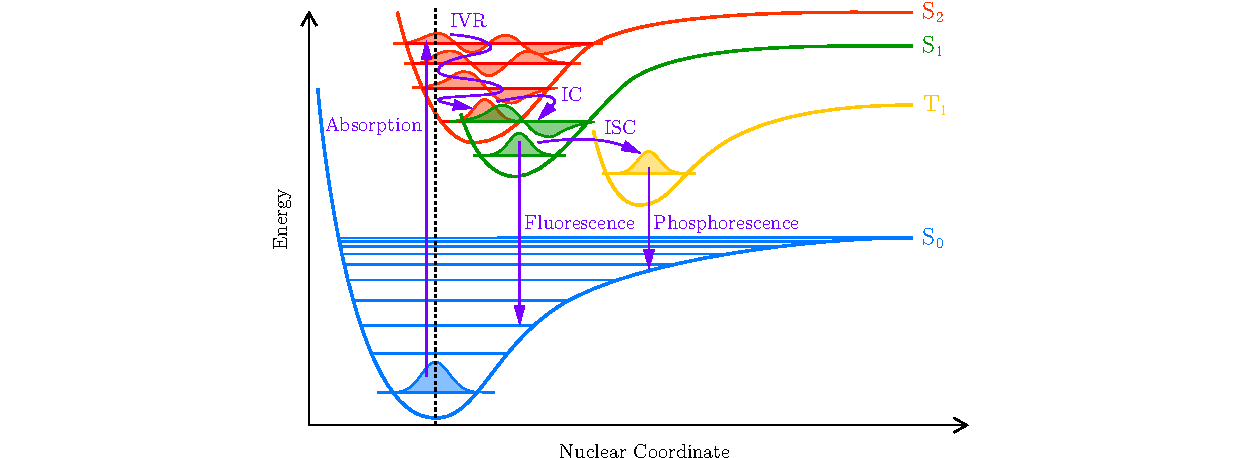
\includegraphics[width = \textwidth]{Figures/fig_ch2_photophysics.pdf}
  \caption[Illustration of the basic photophysical processes
  that can occur when light is absorbed by a molecule
  and the resulting photoexcited state relaxes back to the ground state.]{
  Illustration of the basic photophysical processes that can occur when light is
  absorbed by a molecule and the resulting photoexcited state relaxes back to the ground state.
  The potential energy curves of the first few molecular electronic states are shown:
  the ground state~($S_0$), first and second singlet excited states~($S_1$, $S_2$),
  and first triplet excited state~($T_1$).
  Some of the associated vibrational states are included as wavefunctions
  on a ladder of energy levels to highlight the relevance of wavefunction overlap
  in the Franck-Condon principle.
  Vertical and curved purple arrows indicate radiative and non-radiative transitions respectively;
  Abbreviations: IVR = intramolecular vibrational relaxation, IC = internal conversion,
  ISC = intersystem crossing.
  }
  \label{fig: photophysics}
\end{figure}

In Fig.~\ref{fig: photophysics}, some of the basic photophysical processes that
can be activated during an optical pump-probe experiment are shown.
Light absorption causes a transition from the electronic ground state $S_0$
to some electronic singlet excited state $S_2$.
Here, the Franck-Condon principle%
\footnote{Developed by James Franck (1882--1964) and Edward Condon (1902--1974) in 1926,
this principle states that an electronic transition is
most likely to occur without changes in the nuclear positions and
the transition probability is proportional to the square of the overlap integral between
the two vibrational wavefunctions involved~\cite{Franck1926, Condon1926}.\label{fn: franck-condon}}
determines which vibrational state of $S_2$ is more likely to be occupied initially.
The population of excited molecules can then decay through different
and competing relaxation pathways.
Some, like intramolecular vibrational relaxation~(IVR),
internal conversion~(IC), and intersystem crossing~(ISC), are non-radiative.
They respectively involve transitions between
vibrational states of the same electronic state,
electronic states of the same spin multiplicity, and
electronic states of different spin multiplicities.
Fluorescence and phosphorescence are the radiative equivalents of IC and ISC.
%
An empirical principle known as Kasha's~Rule%
\footnote{Originating from American spectroscopist Michael Kasha~(1920--2013)~\cite{Kasha1950}.
this `rule' is a consequence of the relative density of states
involved in these different types of vibrational-electronic (vibronic) transitions. \label{fn: Kasha}}
orders the time constant~$\tau$ of these transition as follows,
%
\begin{equation}
  \tau_\text{IVR} \ll \tau_\text{IC} \lesssim \tau_\text{ISC}, \tau_\text{F} \ll \tau_\text{P}
\end{equation}
%
Typical values of $\tau$ are shown in Tab.~\ref{tab: transitions} for reference.
%
\begin{table}[t!]
  \centering
  {\renewcommand{\arraystretch}{1.5}
  \begin{tabular}{l c c}
    \toprule
    Transition Process & Pathway & Time Scale~(s)\\
    \midrule
    Absorption & $ S_0 \rightarrow S_n $ & $<10^{-15}$ \\
    Vibrational Relaxation & $ S_n^* \rightarrow S_n $ & $10^{-13}$--$10^{-12}$ \\
    Internal Conversion & $ S_{n} \rightarrow S_{n'} $ & $10^{-14}$--$10^{-11}$ \\
    Intersystem Crossing & $ S_n \rightarrow T_n $ & $10^{-8}$--$10^{-3}$ \\
    Fluorescence & $ S_n \rightarrow S_0 $ & $10^{-9}$--$10^{-8}$ \\
    Phosphorescence & $ T_n \rightarrow S_0 $ & $10^{-3}$--$10^{1}$ \\
    \bottomrule
  \end{tabular}
  }
  \caption{Some general properties of the basic types of electronic transitions~\cite{Jaffe1966}.}
  \label{tab: transitions}
\end{table}

In a TA spectrum, various signals can appear.
%
Negative changes in sample absorption result from either ground state bleach~(GSB),
stimulated emission, or spontaneous emission. The first is a relative increase in
probe-light transmittance caused by depletion of ground-state molecules during pumping.
Stimulated emission is light emitted by electrons in the excited state
whose transition back to the ground state is enhanced by the probe pulse;
in contrast, spontaneous emission stems from probe-independent
radiative relaxation processes (e.g.~fluorescence and phosphorescence) and
are not temporally resolved in TA spectroscopy.
%
Positive changes in absorption are related to
excited state absorption~(ESA) and product state absorption~(PSA),
involving transitions from the excited states populated by the pump pulse to
even higher ones.
%
In addition, a strong signal is usually present
within the time interval when the pump and probe pulses overlap temporally and the combined
laser intensity is high enough to activate a nonlinear process known as
cross-phase modulation~(CPM).%
\footnote{For a more detailed description of CPM, see Ref.~\cite{Islam1987}.}
In Sec.~\ref{sec: TA-data-analysis}, a description is given on how this artifact and others
are removed.
Finally, any other process that changes the energy difference between optically active states
and/or the relevant transition probabilities can give rise to signals in TA data.

\subsection{Experimental Setup}
\label{sec: TA-setup}

The experimental setup for TA spectroscopy is illustrated in Fig.~\ref{fig: TA-setup}.
It is mainly composed of two parts: a commercial femtosecond laser system and
a home-built TA spectrometer.
%
The laser system is composed of
a femtosecond mode-locked laser oscillator (Coherent Micra-5~\cite{MicraManual})
and a titanium-doped sapphire (Ti:Sapph) regenerative amplifier
(REGEN, Coherent Legend Elite~\cite{LegendManual})
along with its high-energy Q-switched pump laser (Coherent Evolution-30~\cite{EvolutionManual}).

\begin{figure}[t!]
  \centering
  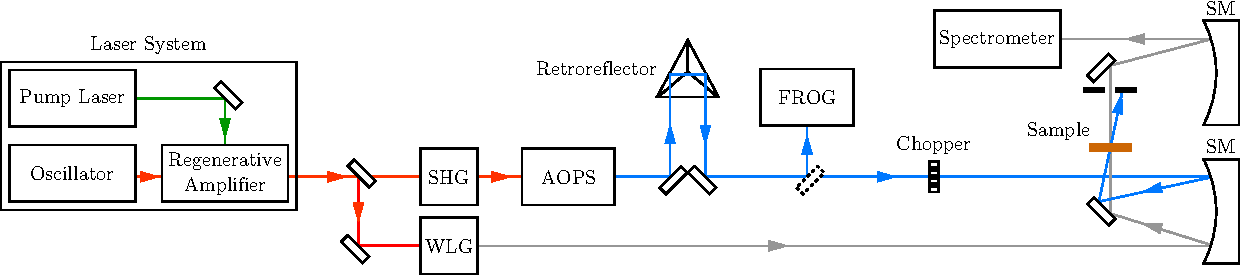
\includegraphics[width = \textwidth]{Figures/fig_ch2_setup-TA.pdf}
  \caption[Schematic of the experimental setup for TA spectroscopy.]{
    Schematic of the experimental setup for TA spectroscopy.
    For simplicity, it is not drawn to scale and minor components are not shown here.
    The directional lines represent optical beam paths and
    their colour denotes the wavelength
    (green = 527 nm, red = 800 nm, blue = 400 nm, and grey = 350--650 nm).
    Abbreviations: SHG = second harmonic generation, WLG = white light generation,
    AOPS = acousto-optic pulse shaper, FROG = frequency-resolved optical gating,
    SM = spherical concave mirror.
  }
  \label{fig: TA-setup}
\end{figure}

During operation, ultrashort seed pulses from the oscillator are strongly amplified in the REGEN
through chirped pulse amplification~(CPA) using light from the pump laser~\cite{Strickland1985}.
%
First light comes from inside the Micra-5 laser:
an intracavity frequency-doubled neodymium-doped yttrium orthovanadate (Nd:YVO\textsubscript{4})
continuous~wave laser (Coherent Verdi) pumps a Ti:Sapph oscillator with green light at 532 nm;
through Kerr-lens mode-locking,%
\footnote{Scottish physicist John Kerr (1824--1907) discovered in 1875 that
the index of refraction of material can be modified by an electric field to the second order:
$\Delta n \propto |\boldsymbol{E}|^2$.
Kerr-lens modelocking involves an optical pulse so intense that it self-focuses
under its own induced $\Delta n$ and is self-selected when coupled with an aperture
that blocks any other mode that fails to self-focus~\cite{BoydBook}.}
weak ultrashort pulses of red light at 800 nm are generated
with a repetition rate of 80 MHz. This pulse train enters the REGEN,
where it is chirped (i.e.~broadened in time) by a grating-based pulse stretcher.
One pulse (out of 8 $\times$ 10\textsuperscript{4}) is selected and injected
into the cavity of the REGEN by a Pockels%
\footnote{German physicist Friedrich Pockels (1865--1913) discovered in 1893 that
the index of refraction of material can be modified by an electric field to the first order:
$\Delta n \propto |\boldsymbol{E}|$. This effect can be used to quickly and precisely control
the polarization of a light beam~\cite{BoydBook}.} cell.
Concurrently, strong green light (537-nm center wavelength, 250-ns pulse duration, 20-mJ pulse energy,
1-kHz repetition rate) from the frequency-doubled
neodymium-doped yttrium lithium fluoride (Nd:YLF) Evolution-30 laser pumps
the Ti:Sapph crystal in the REGEN cavity.
The seed pulse undergoes multiple round trips in the cavity,
accumulating energy from the gain medium each time.
Once the pulse can no longer be further amplified,
it is ejected from the cavity by a second Pockels cell, recompressed by a pulse compressor,
and allowed to leave the REGEN. This output pulse has the following characteristics:
800-nm center wavelength, 35-fs pulse duration, 3.5-mJ pulse energy, and 1-kHz repetition rate.

Light from the laser system is now split into two beams, one going into the `pump' arm
and the other into the `probe' arm of the optical setup. Briefly, the pulses in the former:
frequency-doubled to 400 nm via second harmonic generation~(SHG)%
\footnote{SHG is a nonlinear optical process whereby two photons with the same frequency interact in
a medium to generate a single photon with double the frequency~\cite{BoydBook}.}
in a beta barium borate~(BBO) crystal, compressed using an acousto-optic pulse shaper~(AOPS)~\cite{Dugan1997},
time-delayed by passing through a delay line consisting of a retroreflector mounted on a motorized
translation stage, characterized using a frequency-resolved optical gating device~(FROG)~\cite{Trebino2000},
gated using an optical chopper to set the pump condition, focused onto the sample,
and finally dumped onto a beam block.
%
Simultaneously, the pulses in the probe arm are:
spectrally broadened via white light generation~(WLG)%
\footnote{WLG is the conversion of laser light into light with a very broad spectral bandwidth
(spanning hundreds of nanometers) via strongly nonlinear interactions
in a medium~\cite{Alfano1970, Nagura2002}.}
in a \(\mathrm{CaF_2}\) crystal,
focused onto the sample where it spatially overlaps with the focal spot of the pump beam,
recollimated, and passed into the home-built spectrometer.
%
With the exception of the laser system, the entire experimental setup here
was designed and built by Dr.~Ryan L. Field as part of his doctoral project.
Further details can be found in his thesis~\cite{Ryan-thesis}.

\subsection{Data Analysis}
\label{sec: TA-data-analysis}

During a TA experiment, there are significant features
in the data that are caused by optical processes of no present interest. They are artifacts
that need to be removed before the $\Delta A(t, \lambda)$ measurements are studied too closely.
In Fig.~\ref{fig: TA-Clean}, sample TA data at different stages of artifact removal
are shown and the parameters used to quantify the contribution of the artifacts are plotted alongside.
%
\begin{figure}[t!]
  \centering
  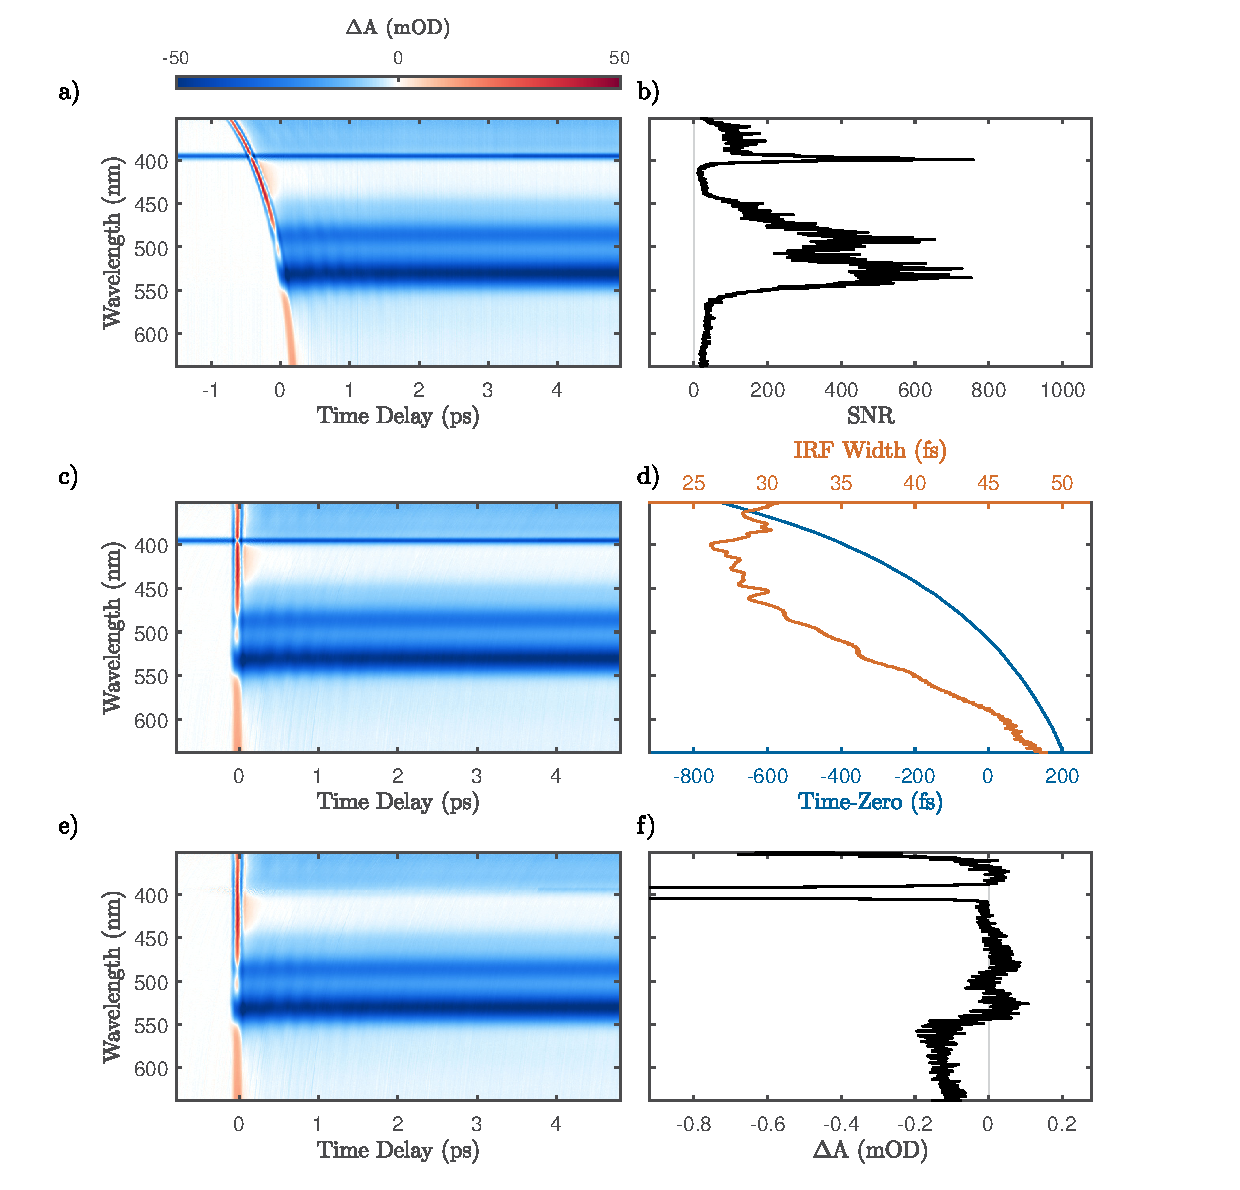
\includegraphics[width = \textwidth]{Figures/fig_TA_cleanup.pdf}
  \caption[Illustration of the steps for artifact removal in TA data.]{
  Illustration of the steps for artifact removal in TA data.
  Step 1: (a) restrict TA data to wavelength regions where $\textrm{SNR}(\lambda) > 5$
  using (b) the SNR estimated from Eq.~\eqref{eq: mu-sigma-SNR} for all probed wavelengths.
  Step 2: (c) correct the GVD distortion of the TA data
  by reversing (d) the wavelength dependence of the time-zero and IRF~width
  derived from a Hermite fitting of the CPM signal as in Eq.~\eqref{eq: CPM-fit}.
  Step 3: (e) obtain the final artifact-free TA data by
  (f) integrating and then subtracting all pre-CPM signals via Eq.~\eqref{eq: pre-signal}.
  }
  \label{fig: TA-Clean}
\end{figure}

The first step is the removal of regions of low signal-to-noise ratio~(SNR)
in the wavelength domain. This is caused by the fact that the bandwidth of white-light probe
is finite and there is not enough light beyond to differentiate signal from noise (see Fig.~\ref{fig: BPY-data-whitelight}).
Here, the SNR is estimated to be the ratio of the mean~$\mu$ to the standard deviation~$\sigma$
of the differential absorbance measurements at late time delays $t \in [t', t'']$,
when all transient signals have decayed completely:
%
\begin{equation}
  \begin{aligned}
    \mu(\lambda) & = \frac{1}{T} \int_{t'}^{t''} \Delta A(t, \lambda) \mathrm{d}t  \\
    \sigma(\lambda) & = \sqrt{\frac{1}{T} \int_{t'}^{t''} \left( \Delta A (t, \lambda) - \mu(\lambda) \right)^2 \mathrm{d}t}
    \label{eq: mu-sigma-SNR}
  \end{aligned}
\end{equation}
%
where $T = t'' - t'$.
A window is then applied on the TA data by limiting its wavelength domain to an interval
in which the SNR is above a threshold value,
$\lambda \rightarrow \lambda \in \left\{ \lambda \mid \textrm{SNR}(\lambda) > 5 \right\}$.

Next, the wavelength-dependent shift in time-zero%
\footnote{`time-zero' is the time delay at which there is temporal overlap of the pump and probe pulses.}
is considered. This varying arrival time of the probe pulse is caused by group velocity dispersion~(GVD)
that occurs when the broadband probe light propagates through transmissive optical elements
of the experimental setup. To quantify this effect, TA measurements are made on samples%
\footnote{For the experiments described in Sec.~\ref{sec: TA-BPY}, the non-resonant samples
are just blank sample media: deionized water in a quartz flow cell for the aqueous case,
a sapphire window for the crystal case.} that are not resonant
within the probe wavelength region~(see Ref.~\cite{Ryan-thesis} for more details).
The correct time-zero~$t_0(\lambda)$ is estimated by fitting
the CPM~signal $\Delta A_\textrm{CPM}(t, \lambda)$ with a model function that is
a linear combination of the first four Hermite polynomials~$H_n$ for each wavelength:
%
\begin{equation}
  \textrm{C}(t, \lambda, \{a_n\}, t_0, \tau) =
    \sum_{n = 0}^4 a_n(\lambda) H_n(x) \Bigg\rvert_{x = (t - t_0(\lambda))/\tau(\lambda)}\\
  \label{eq: CPM-fit}
\end{equation}
%
Then, each time series of the sample data is translated temporally
such that all the time-zeros are aligned: $\Delta A(t, \lambda) \rightarrow \Delta A(t - t_0, \lambda)$.
For time-zero shifts which are not integer multiples of the time delay step size,
super-resolution alignment is achieved through spline interpolation.
Incidentally, the parameter $\tau(\lambda)$ corresponds to the temporal width
of the instrument response function (IRF)%
\footnote{The IRF here is assumed to be Gaussian, given that it is a convolution of
the nearly Gaussian temporal profile of the pump and probe pulses.} of the experimental
setup~\cite{Megerle2009}.

Another TA artifact is the negative signals caused by scattered pump light
and fluorescence from the sample. Since they occur independently of the probe pulse
and their amplitude is mostly determined by the geometry of the experimental setup,
they are present and nearly constant at all time delays. Thus, they are
removed by averaging the pre-CPM differential absorbance and subtracting it
from the rest of the TA values:
%
\begin{equation}
  \Delta A(t, \lambda) \rightarrow \Delta A(t, \lambda) - \frac{1}{T}\int_{t'}^{t''} \Delta A(t, \lambda) \mathrm{d} t
  \label{eq: pre-signal}
\end{equation}
%
where $t \in [t', t'']$ and $T = t'' - t'$ refer to the time delay interval before time-zero
during which the CPM~signal is not yet present

Now that the TA data is artifact-free, a technique known as global analysis (GA)
is applied to reduce $\Delta A(t, \lambda)$ into a sum of exponentially decaying
spectral components that could be assigned to specific electronic states
and photophysical processes~\cite{Nagle1991, Grondelle2004, Wilderen2011, Ruckebusch2012}.
The first step of GA is to recognize that $\Delta A(t , \lambda)$ is just a
$ M \times N$ data matrix $\mathbf{\Delta \! A}$, where $M$ and $N$ are the number of wavelength
and time points respectively,
%
\begin{equation}
\begin{aligned}
  %t & = \{ t_1, ..., t_N \} \\
  %\lambda & = \{ \lambda_1, ..., \lambda_M \} \\
  \Delta A(t, \lambda) \rightarrow \mathbf{\Delta \! A} =
  \begin{bmatrix}
      \Delta A(t_1, \lambda_1) & \cdots & \Delta A(t_N, \lambda_1) \\
      \vdots & \ddots & \vdots \\
      \Delta A(t_1, \lambda_M) & \cdots & \Delta A(t_N, \lambda_M)
  \end{bmatrix}
\end{aligned}
\end{equation}
%
and it can be factored using singular value decomposition~(SVD) into
separate spectral and temporal features:
%
\begin{equation}
  \mathbf{\Delta \! A} = \mathbf{U} \mathbf{S} \mathbf{V}^\mathsf{T}
\end{equation}
%
where $\mathbf{U} = U(\lambda)$ and $\mathbf{V} = V(t)$ are
orthogonal matrices of size $M \times M$ and $N \times N$ respectively;
$\mathbf{S}$ is a $M \times N$ diagonal matrix of rank $P$.
This factorization can be rewritten to give an expansion of $\mathbf{\Delta \! A}$
as a weighted ordered sum of `singular components' $\mathbf{X}_i$:
%
\begin{equation}
  \begin{aligned}
    \mathbf{\Delta \! A} & = \sum_{i = 1}^P s_i \mathbf{X}_i \\
    \mathbf{X}_i & = \mathbf{u}_i \otimes \mathbf{v}_i^\mathsf{T}
    \label{eq: TA SVD sum}
  \end{aligned}
\end{equation}
%
where $\mathbf{u}_i = u_i(\lambda)$ and $\mathbf{v}_i = v_i(t)$
are the column vectors of $\mathbf{U}$ and $\mathbf{V}$; they are known as
the left and right `singular vectors' and, specifically in TA, the `basis spectra'
and `kinetic traces' of the overall dataset, respectively; $s_i$ is defined as the diagonal entries of $\mathbf{S}$
and known as the `singular values' of the data matrix.
In general, the set of singular values is sorted in descending order and
an approximation of the data matrix can be obtained by truncating this summation
at some $P' \ll P$, thus keeping only those singular components that contribute
significantly to the overall signal. This concept is particularly useful in
deconvolving incoherent noise from signals and it is illustrated in Figure~\ref{fig: TA-SVD}.

\begin{figure}[t!]
  \centering
  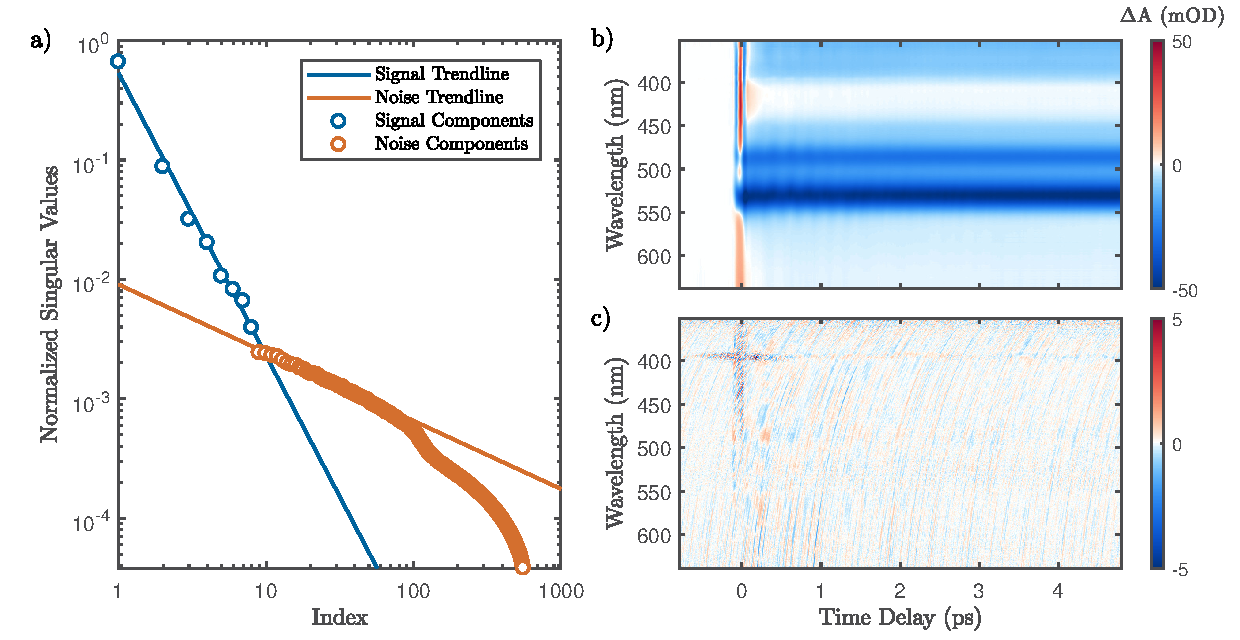
\includegraphics[width = \textwidth]{Figures/fig_TA_svd.pdf}
  \caption[Demonstration of a low-rank approximation of a TA data matrix using SVD.]{
  A low-rank approximation of a data matrix using SVD, as per Eq.~\eqref{eq: TA SVD sum},
  is demonstrated using the TA data shown in Fig.~\ref{fig: TA-Clean}f.
  The contribution of each singular component $\mathbf{X}_i$ is weighted by
  the associated singular value $s_i$,
  which is shown here on a log-log plot in (a)~after normalization.
  Two linear trendlines can be fitted piecewise to this curve; they are overlain
  to highlight the sudden change in slope as the normalized singular values decay to zero.
  Summing the singular components before and after this flexion yields
  the $\Delta A(t, \lambda)$ values in Panels~(b) and (c) respectively.
  By inspection, it is clear that the index at which the flexion occurs marks
  the point beyond which the remaining $\mathbf{X}_i$ only contribute irrelevant features
  and incoherent noise.
  }
  \label{fig: TA-SVD}
\end{figure}

After SVD and truncation, the TA dataset is now reduced to
a few basic spectra~$u_i(\lambda)$ and kinetic traces $v_i(t)$.
These are not readily interpretable in terms of photophysical processes
since they are only orthogonal bases that jointly span the data matrix.
To proceed further, a global lifetime analysis~(GLA) fit is done by assuming
an exponential model for the population dynamics of optically active species.
Each kinetic trace is assumed to be a weighted sum of $Q$ exponential decay functions
switched on at time-zero by a Heaviside step function $H(t)$ and convolved with a Gaussian IRF
whose temporal width $\tau_\text{IRF}$ is obtained earlier by fitting the response of
a non-resonant sample (see Fig.~\ref{fig: TA-Clean}f);
as before, the CPM~signal is described by a linear combination of the first four Hermite polynomials $H_n(t)$,
%
\begin{equation}
  \begin{aligned}
    C_i(t, \{a_{i n}\})
      & = \sum_{n = 0}^4 a_{i n}(\lambda) H_n \left( t/\tau_{\text{IRF}} \right)  \\
    \textrm{IRF}(t)
      & = \text{e}^{-\frac{1}{2} t^2/ \tau_\text{IRF}^2}  \\
    E_i(t, \{ b_{i j}\}, \{k_j\})
      & = \sum_{j = 1}^Q b_{i j} \left( H(t) \text{e}^{-k_j t}\right) \ast \text{IRF}(t) \nonumber\\
    f_i(t, \{a_{i n}\}, \{ b_{i j}\}, \{k_j\})
      & = C_i(t, \{a_{i n}\}) + E_i(t, \{ b_{i j}\}, \{k_j\})
    \label{eq: GA fit}
  \end{aligned}
\end{equation}
%
where $f_i$, $C_i$ and $E_i$ are the model functions for the kinetic trace $\boldsymbol{v}_i(t)$, and
its CPM and exponential contributions.%
\footnote{For reference,
$ \left( H(t - t_0) \text{e}^{-k t}\right) \ast \text{e}^{- \frac{1}{2} t^2/\tau^2} =
\frac{1}{2} \text{e}^{\frac{1}{2} k^2 \tau^2 - k (t - t_0)}
\left( 1 +
\text{erf}\left( \frac{t - t_0 - k \tau^2}{\sqrt{2} \tau} \right)
\right)$.
} To track the changes in $\Delta A$ that are associated with each exponential process,
a decay-associated spectrum (DAS) $D_j(\lambda)$ for each decay constant $k_j$
is calculated as a linear combination of the basis spectra $u_i(\lambda)$
weighted by the fitted amplitude $b_{i j}$ and singular values $s_i$:
%
\begin{equation}
  D_j(\lambda) = \sum_{i = 1}^{P'} b_{ij} s_i u_i(\lambda)
  \label{eq: DAS}
\end{equation}
%
This calculation is demonstrated using the TA data in Fig.~\ref{fig: TA-SVD}b and
the results are plotted in Fig.~\ref{fig: TA-GLA}.
%
\begin{figure}[ht!]
  \centering
  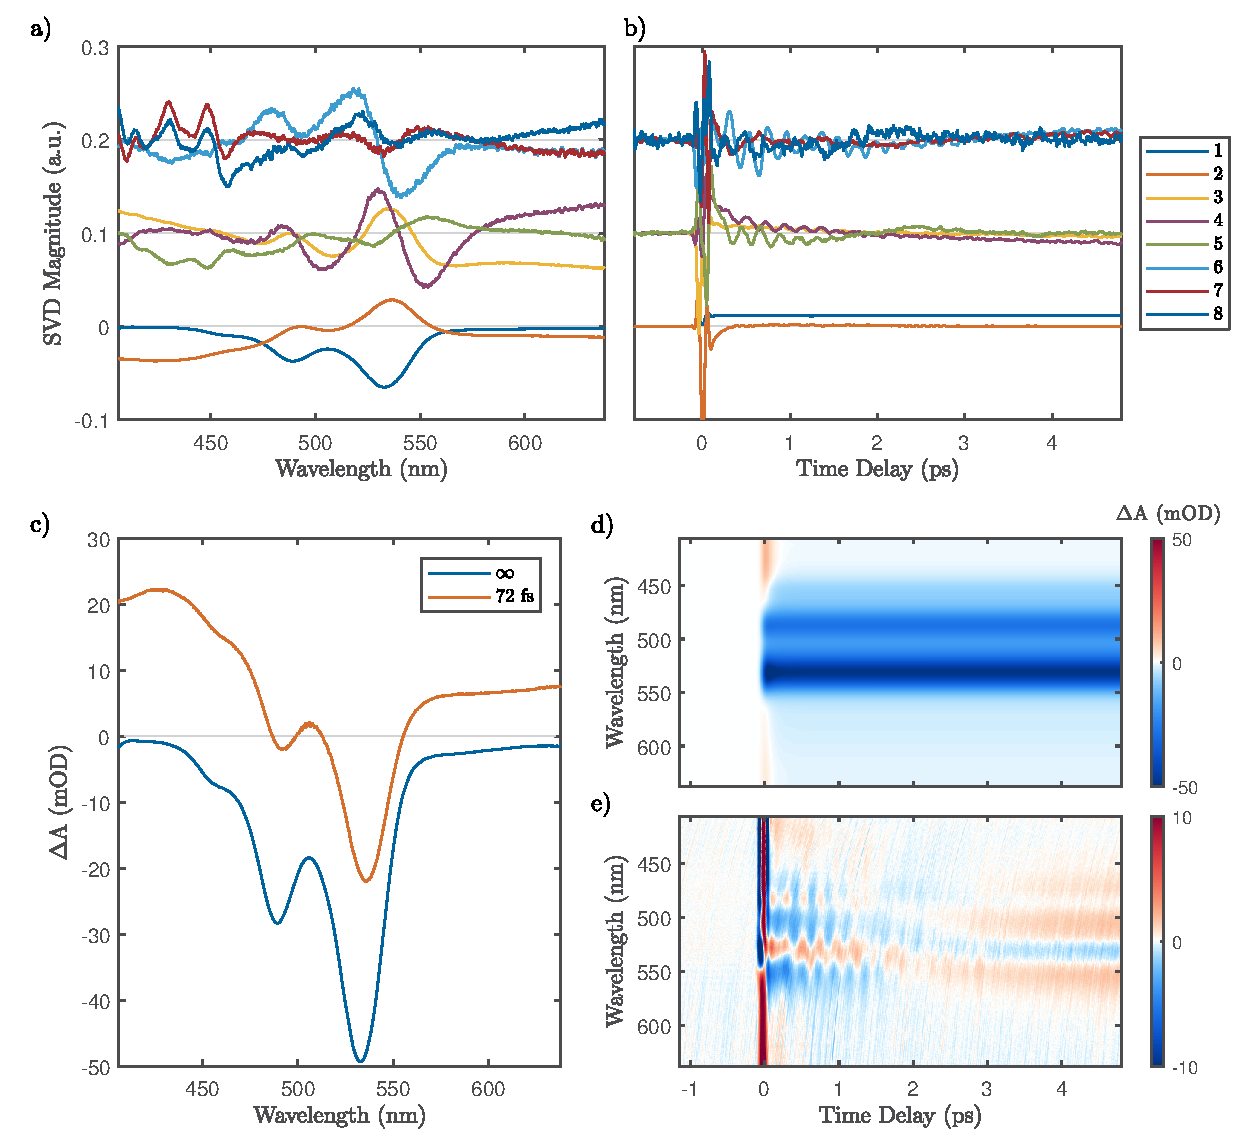
\includegraphics[width = \textwidth]{Figures/fig_TA_GLA.pdf}
  \caption[Truncation of a SVD sum at the point of flexion.]{
    Truncating the SVD sum of the TA data matrix (from Fig.~\ref{fig: TA-SVD}c)
    at the point of flexion leaves (a)~eight principal basis spectra and (b)~eight kinetic traces
    in the TA data matrix. Two exponential components ($\tau_1$ = $\infty$, $\tau_2$ = 72 fs)
    are needed for the GLA~fit of the kinetic traces (Eq.~\eqref{eq: GA fit})
    and their respective DAS (Eq.~\eqref{eq: DAS}) are plotted in Panel~(c).
    The resulting global fit and residuals are shown in Panels~(d) and (e).
  }
  \label{fig: TA-GLA}
\end{figure}
%
Finally, the global fit $G(t, \lambda)$ (as shown in Fig.~\ref{fig: TA-GLA}d)
are calculated by recombining each $D_j(\lambda)$ with
its corresponding exponential function with decay constant $k_j$:
%
\begin{equation}
  G(t, \lambda) = \sum_{j = 1}^{Q} D_j(\lambda) \left[  \left( H(t) \text{e}^{-k_j t}\right) \ast \textrm{IRF}(t) \right]
\end{equation}
%
The residuals of the fit, $R(t, \lambda) = \Delta A(t, \lambda) - G(t, \lambda)$, contain
signals not captured by the exponential model. As seen in Fig.~\ref{fig: TA-GLA}e, these features
include the CPM near time-zero, lattice heating effects at late times, and various oscillatory dynamics
in between. For the latter, relevant frequencies can be extracted by calculating
the power spectrum of the residuals at each probe wavelength
using Welch's method for spectral density estimation~\cite{Welch1967}
or a continuous wavelet transform (see Sec.~\ref{sec: freq-anal-BPY}).


%%%%%%%%%%%%%%%%%%%%%%%%%%%%%%%%%%%%%%%%%%%%%%%%%%%%%%%%%%%%%%%%%%%%%%%%%%%%%%%%%%%%%%%%%%%%%%%%%%%%%%

\section{Ultrafast Electron Diffraction}
\label{sec: UED}

Since its discovery in 1923--1927~\cite{Gehrenbeck1978}, electron diffraction became
an indispensable weapon in the arsenal of those seeking to
investigate the structure of materials on the atomic level.
%
The advent of time-resolved laser spectroscopy and the introduction of the pump--probe methodology
involving ultrashort pulses to this technique further extended its capabilities,
which now includes the study of ultrafast atomic motions and structural dynamics
during physico-chemical processes,
hence conferring it the titular specialization of ultrafast electron diffraction~(UED).

Given the roots of UED, some basic tenets of crystallography and electron scattering physics
is necessary to fully understand UED as an experimental technique and interpret its measurements.
%
As such, a brief introduction to these two topics ---
based on Refs.~\cite{AshcroftBook, EwaldBook, XRDBook, WarrenBook}
and~\cite{TownsendBook, CowleyBook, ReimerBook, KirklandBook, ZouBook, Giacovazzo2011} ---
is given as follows.

\subsection{Overview of Crystallography}
\label{sec: UED-cryst}

A common feature of physical objects is that
their constituent atoms are not distributed randomly
but are bound together as molecules and arranged in a regular periodic array.
Materials structured as such are known as crystals%
\footnote{Since the discovery of `quasicrystals' in 1984 by Israeli material scientist
Daniel Shechtman (1941--present)~\cite{Shechtman1984}, crystals are now more accurately described as
``any solids having an essentially discrete diffraction diagram''
wherein 3D~periodicity may be absent~\cite{IUC1992}.} and
they are the subject of study for crystallographers.

A fundamental concept to describe crystal structures is the `Bravais lattice',%
\footnote{Moritz L. Frankenheim (1801--1869) first discovered in 1826 that
they are no more than 15 distinct types of lattices in three dimensions.
Auguste Bravais (1811--1863) later correctly revised this number to 14~\cite{XRDBook}.}
which is an infinite array of points that maps back onto itself
under discrete translations in three-dimensional space.
The position of every point in a Bravais lattice can be stated as
$\boldsymbol{R} = n_1 \boldsymbol{a}_1 + n_2 \boldsymbol{a}_2 + n_3 \boldsymbol{a}_3$,
where $n_j$ are integers and $\boldsymbol{a}_j$
are the three non-coplanar primitive vectors that generate the lattice.
The region of space spanned by the vectors $\boldsymbol{a}_j$
is known as the `unit cell' of the lattice;
it is the spatial volume that is repeated throughout the lattice
and preserved under its translational symmetry.
Although there is no unique way to choose the primitive vectors and
the unit cell of a lattice,
the conventional approach is to pick the most orthogonal set of
lattice-generating vectors and the parallelepiped in the first octant
of the resulting coordinate system.
As seen in Fig.~\ref{fig: unit-cell}a, the unit cell and its primitive vectors are specified
by a set of six lattice parameters%
\footnote{In conventional crystallographic notation, the six lattice parameters are
denoted by $a, b, c, \alpha, \beta, \gamma$ respectively.
Here, this is done using the index notation for convenience.}:
the length of the three vectors ($a_1, a_2, a_3$)
and the internal angles ($\alpha_{23}, \alpha_{31}, \alpha_{12}$),
where $\cos \alpha_{ij} = | \hat{\boldsymbol{a}}_i \cdot \hat{\boldsymbol{a}}_j|$.
Herein, the components of $\boldsymbol{a}_j$ can be expressed as
%
\begin{equation}
\begin{aligned}
  \boldsymbol{a}_1 & = a_1 \left[ 1 \quad 0 \quad 0 \right]  \\
  \boldsymbol{a}_2 & = a_2 \left[ \cos \alpha_{12} \quad \sin \alpha_{12} \quad 0 \right] \\
  \boldsymbol{a}_3 & = a_3 \left[ \cos \alpha_{31} \quad \frac{\cos \alpha_{23} - \cos \alpha_{31} \cos \alpha_{12}}{\sin \alpha_{12} } \quad \frac{V}{a_1 a_2 a_3 \sin \alpha_{12}} \right]
\end{aligned}
\end{equation}
%
where $V$ is the volume of the unit cell,
%
\begin{equation}
\begin{aligned}
  V & = \left| \boldsymbol{a}_1 \cdot (\boldsymbol{a}_2 \times \boldsymbol{a}_3) \right| \\
    & = a_1 a_2 a_3 \sqrt{1 + 2 \cos \alpha_{23} \cos \alpha_{31} \cos \alpha_{12} - \cos^2 \alpha_{23} - \cos^2 \alpha_{31} - \cos^2 \alpha_{12}}
\end{aligned}
\end{equation}

\begin{figure}[t!]
  \centering
  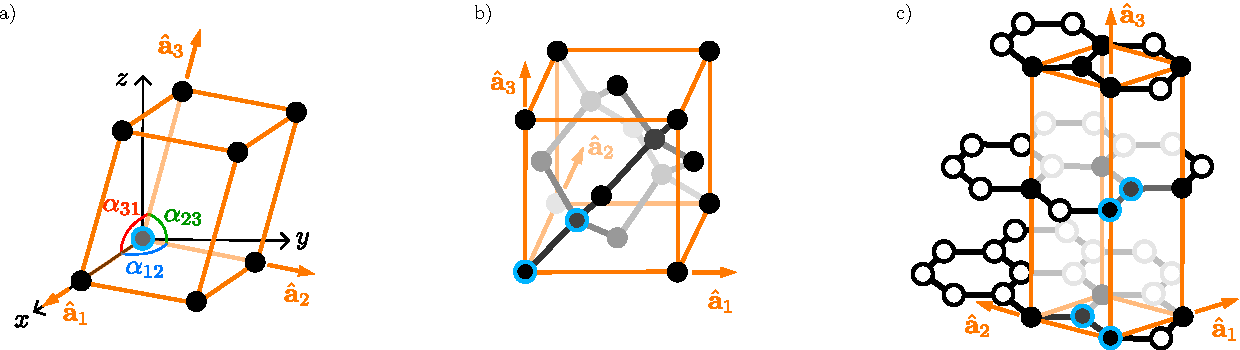
\includegraphics[width = \textwidth]{Figures/fig_ch2_unitcell.pdf}
  \caption[Crystal structures as described by their Bravais lattice.]{
    Crystal structures as described by a Bravais lattice and an associated basis.
    The unit cell is orange parallelepiped; atoms inside/outside are filled/empty circles;
    the basis atoms are outlined in blue.
    (a)~The six parameters ($a_1, a_2, a_3, \alpha_{23}, \alpha_{31}, \alpha_{12}$)
    that specify the shape of an unit cell are defined.
    The crystal structures of (b)~diamond and (c)~hexagonal graphite are depicted.
    The first is a face-centered cubic lattice with a two-atom basis;
    the second is a hexagonal lattice with a four-atom basis.
  }
  \label{fig: unit-cell}
\end{figure}

The structure of a physical crystal can be described
by a Bravais lattice wherein the repeating arrangement of atoms
is enclosed within the volume of a particular unit cell and
this subset of atoms defines a `basis' relative to each lattice point.
Under this scheme, the position of any atom $j$ in the crystal is given by
$\boldsymbol{r}_j = \boldsymbol{R}_{n_1 n_2 n_3} + \boldsymbol{\scriptr}_i$,
where $\boldsymbol{R}_{n_1 n_2 n_3} = \sum \limits_{j = 1}^3 n_j \boldsymbol{a}_j$
is the position of the lattice point to which the origin of the unit cell is defined
and $\boldsymbol{\scriptr}_i$ is the position of the basis atom $i$ that is equivalent
to atom $j$ under symmetry.

The facets of the crystal are related to families of parallel equidistant planes
which intersect the Bravais lattice at (at least) three non-collinear lattice points.
Within the unit cell, such a lattice plane has intercepts $\frac{a_j}{h_j}$ on the three lattice vectors
and can be specified by the notation $(h_1 h_2 h_3)$, where $h_j$ are coprime integers
(see Fig.~\ref{fig: reciprocal-laue-bragg}a) and they are known as the `Miller indices'%
\footnote{William H. Miller (1801--1880) introduced this notation for crystal planes in 1839.
The letters $h, k, l$ are used therein most often;
however, the labels $h_1, h_2, h_3$ are used instead here for convenient indexing.
An overline indicates a negative number, $\overline{h} = -h$.} of the plane.
A set of vectors can be constructed%
\footnote{A computationally more useful definition of the reciprocal lattice vectors is
$ \left[ \boldsymbol{b}_1 \boldsymbol{b}_2 \boldsymbol{b}_3 \right] = 2 \unslant[-.2]\pi \left[ \boldsymbol{a}_1 \boldsymbol{a}_2 \boldsymbol{a}_3 \right]^{-1}$,
where the vectors are in column representation.}
as $\boldsymbol{b}_i = \frac{\unslant[-.2]\pi}{V} \sum \limits_{j,k = 1}^3 \epsilon_{ijk} \enskip \boldsymbol{a}_j \times \boldsymbol{a}_k$,
where $\epsilon_{ijk}$ is the Levi-Civita symbol.
%
Under this definition, the three vectors $\boldsymbol{b}_i$ have the property of
$\boldsymbol{b}_i \cdot \boldsymbol{a}_j = 2 \unslant[-.2]\pi \delta_{ij}$, where $\delta_{ij}$ is the Kronecker delta,
with the corollary $|\boldsymbol{b}_i| = 2\unslant[-.2]\pi / |\boldsymbol{a}_i|$.
%
Since their magnitude is the reciprocal of that of the crystal lattice and
they can generate their own Bravais lattice
where each vector $\boldsymbol{g} = \sum \limits_{i = 1}^3 h_i \boldsymbol{b}_i$,
the vectors $\boldsymbol{b}_i$ are known as `reciprocal lattice vectors';
the reciprocal vector $\boldsymbol{g}$ corresponds to the normal of a plane $(h_1 h_2 h_3)$
in the `direct lattice' (as opposed to the reciprocal lattice)
and its magnitude is proportional to the reciprocal of the interplanar distance $d_{h_1 h_2 h_3}$,
$| \boldsymbol{g} | = 2\unslant[-.2]\pi/d_{h_1 h_2 h_3}$.
This geometric relationship between planes in the crystal lattice and
points in the reciprocal lattice provides a convenient basis to discuss
the interference of waves reflected by the bulk crystal.
%
\begin{figure}[t!]
  \centering
  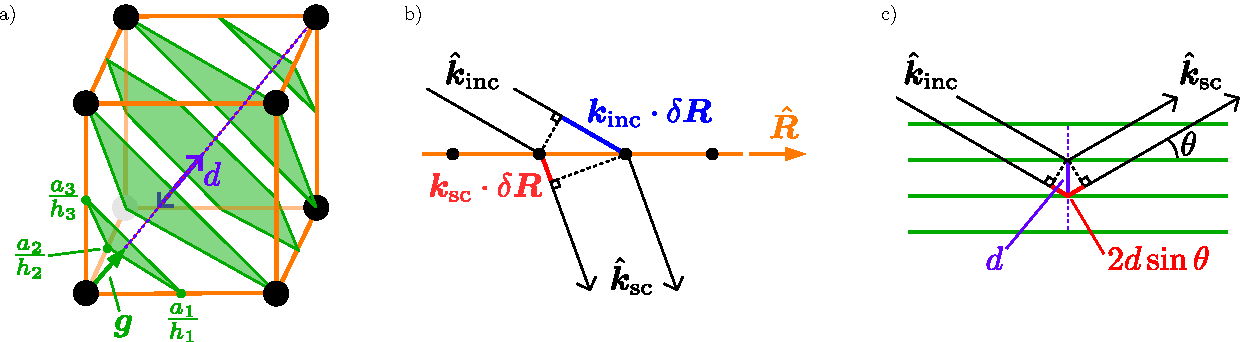
\includegraphics[width = \textwidth]{Figures/fig_ch2_reciprocal-laue-bragg.pdf}
  \caption[Diffraction according to Max v. Laue and William L. Bragg.]{
    (a) Family of lattice planes specified by the Miller indices $h_1, h_2, h_3 = 2$ is depicted,
    along with the reciprocal lattice vector $\boldsymbol{g}$ that corresponds to the normal of the planes.
    The path difference that leads to diffraction in crystals is shown
    according to the formulation of (b)~Max v. Laue and (c)~William L. Bragg.
  }
  \label{fig: reciprocal-laue-bragg}
\end{figure}

When a wave penetrates a material, new waves are produced through scattering and
they can interact with the original wave. In the case of a crystal, the periodic features
that underlie the crystal structure generate many scattered waves with discrete phase differences.
Under certain conditions, there is constructive interference between these waves and the incident one
and diffraction occurs. There are two formulations of these diffraction conditions:
one conceived by Max v. Laue and the other by William L. Bragg, both%
\footnote{Max v. Laue (1879--1960) was awarded the 1914 Nobel Prize in Physics for
the discovery of X-ray diffraction.
William L. Bragg (1890--1971), along with his father William H. Bragg (1862--1942),
won the same award in 1915 for their work in X-ray crystallography~\cite{Nobel1901}.} in 1912.
As seen in Fig.~\ref{fig: reciprocal-laue-bragg}b,
the first approach considers the crystal to be lines of scatterers,
equally spaced by $\delta \boldsymbol{R} = \boldsymbol{a}_j$;
assuming elastic scattering,
the phase difference between the transmitted wave and the scattered one
is $\Delta \phi = (\boldsymbol{k}_{\text{sc}} - \boldsymbol{k}_{\text{inc}}) \cdot \delta \boldsymbol{R}$
and thus, the Laue condition for diffraction is
%
\begin{equation}
  \boldsymbol{q} \cdot \boldsymbol{a}_j = 2 \unslant[-.2]\pi h_j
  \label{eq: laue}
\end{equation}
%
where $\hbar \boldsymbol{q} = \hbar(\boldsymbol{k}_{\text{sc}} - \boldsymbol{k}_{\text{inc}})$
is the momentum transferred during the scattering event and $h_j$ are integers.
In the Bragg formulation (Fig.~\ref{fig: reciprocal-laue-bragg}c), the crystal is composed of parallel reflective planes
evenly separated by the interplanar distance $d$; the incident wave interferes
with the reflected waves only if the path difference is an integer multiple $n$ of the wavelength $\lambda$
and hence the Bragg condition for diffraction is
%
\begin{equation}
  2 d \sin \theta = n \lambda
  \label{eq: bragg}
\end{equation}

The Laue and Bragg conditions are equivalent and this can be shown
by noting that the Laue condition effectively constrains
diffraction to only occur for $\boldsymbol{k}_\text{sc}$ such that
$\boldsymbol{q}$ is an integer multiple of a reciprocal lattice vector $\boldsymbol{g}$ of the crystal.
A helpful way to interpret these conditions is through
a geometric construct%
\footnote{Paul P. Ewald (1888--1985) conceived of the sphere-in-reciprocal-lattice construct
to geometrically visualize diffraction in 1912~\cite{EwaldBook}.} known as the `Ewald sphere'.
In the space of wavevectors, the reciprocal lattice
and a sphere --- centered on $\boldsymbol{k}_\textrm{inc}$ and
of radius $|\boldsymbol{k}_\textrm{inc}|$ ---
are drawn such that the latter is tangential to the lattice origin.
The surface of this sphere represents all possible elastic scattering events
such that $|\boldsymbol{k}_\textrm{sc}| = |\boldsymbol{k}_\textrm{inc}|$.
As seen in Fig.~\ref{fig: ewald}, the locations on the surface of the Ewald sphere that overlap
with any points of the reciprocal lattice specifies those scattering geometries
wherein the transfer wavevector $\boldsymbol{q}$ and the scattering $\theta$
satisfy the Laue and Bragg conditions respectively.
Propagating these beams onto the detector yields
the spots of the diffraction pattern that can be expected by an observer in real space.
%
\begin{figure}[t!]
  \centering
  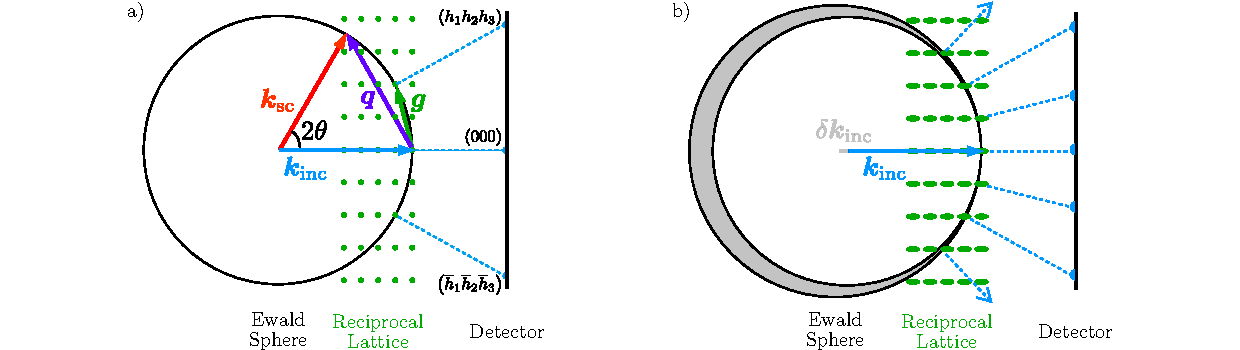
\includegraphics[width = \textwidth]{Figures/fig_ch2_ewald.pdf}
  \caption[Construction of the Ewald sphere.]{
    Construction of the Ewald sphere.
    (a)~The Laue-Bragg condition is satisfied at scattering angles $\theta$
    where the surface of the sphere coincides with reciprocal lattice points $\boldsymbol{g}$;
    when projected onto the detector, these points indicate where diffraction spots may be observable.
    (b)~Realistic incident beams with nonzero energy and momentum spreads,
    in addition to finite and imperfect crystals,
    loosen the condition for diffraction and lead to more diffraction spots
    than would otherwise be expected.
  }
  \label{fig: ewald}
\end{figure}

In a perfect, infinite, and static crystal,%
\footnote{A `perfect' crystal is one with unbroken discrete translational symmetry;
`infinite' refers to the absence of boundaries, and `static', a lack of atomic motion.}
few if any diffraction spots would be observable
for a general monochromatic incident beam.
It is unlikely that any integer solution $(h_1 h_2 h_3)$,
other than the transmitted beam at $(000)$,
exactly satisfies the Laue-Bragg condition.
In practice, incident beams are not composed of
perfectly coherent waves;
the resulting nonzero energy and momentum spread manifest
within the Ewald construct (Fig.~\ref{fig: ewald}b)
as a thickening the surface of the sphere into a shell
that can overlap with many more reciprocal lattice points.
Furthermore, the finite dimensions and long-range disorder
of the crystal effectively broaden the points into extended spikes%
\footnote{These shapes are known in the literature as
reciprocal lattice rods, or `relrods' for short.}
that can more easily be intercepted by the Ewald sphere.
Hence, experimental imperfections ensure that
the requirements of diffraction are sufficiently relaxed
for a multitude of spots to appear in a diffraction pattern.

\begin{figure}[ht!]
  \centering
  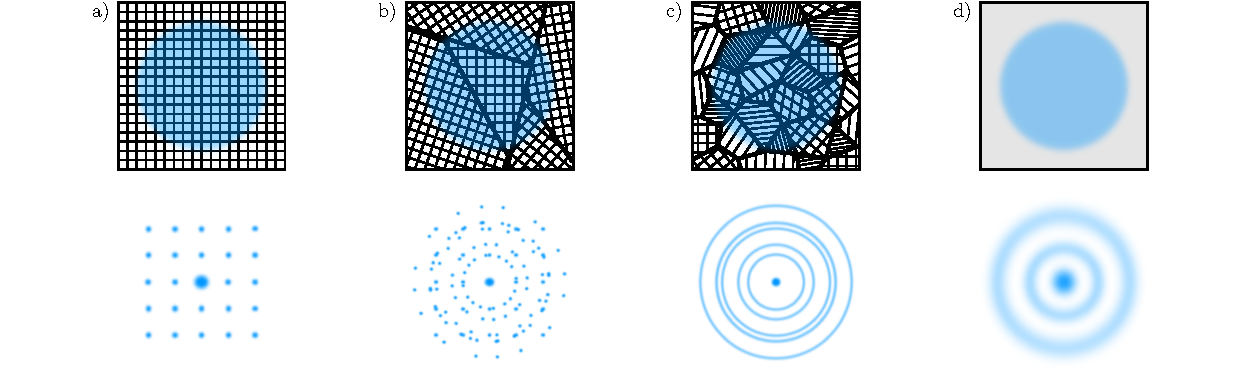
\includegraphics[width = \textwidth]{Figures/fig_ch2_crystal-powder-diff.pdf}
  \caption[Samples of varying crystallinity and the resulting diffraction patterns.]{
    Samples of varying crystallinity and the resulting diffraction patterns:
    (a)~a perfect single crystal, (b)~a polycrystal, (c)~a powder,
    and (d)~an amorphous sample.}
  \label{fig: crystal-powder-diff}
\end{figure}

A diffraction pattern does not necessarily appear as
the regular array of spots that the Ewald construct would suggest.
The nature of the pattern can be an indication of the crystallinity
of the target. As shown in Fig.~\ref{fig: crystal-powder-diff},
a perfect single crystal gives a periodic arrangement of diffraction spots
while fluids and amorphous%
\footnote{An amorphous material is one that lacks the long-range order of
a crystal.} materials produce highly diffuse rings centered around the transmitted beam.
%
In between these two extremes in structural order,
there are coarse- and fine-grained polycrystalline materials
wherein the individual randomly-oriented crystallites contribute
their own diffraction spots that sum to a set of spotty concentric circles,
generally known as Debye-Scherrer%
\footnote{Paul Scherrer (1890--1969), under the guidance of Peter Debye (1884--1966), and
Albert W. Hull (1880--1966) developed in 1915--1917 the method for analyzing
X-ray crystal structures using powder samples
instead of single-crystal ones~\cite{EwaldBook, DebyeScherrer2011}.
\label{fn: debye-waller}} rings.

\subsection{Physics of Electron Scattering}
\label{sec: UED-physics}

\begin{figure}[ht!]
 \centering
 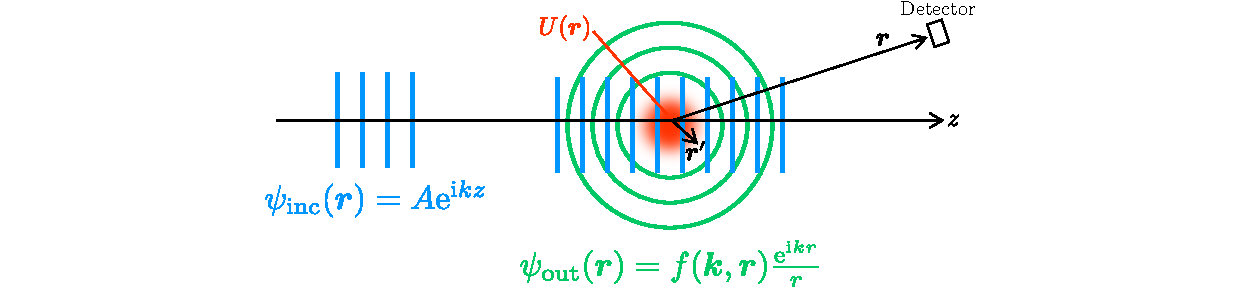
\includegraphics[width = \textwidth]{Figures/fig_ch2_electron-scatter.pdf}
 \caption{
  Schematic of the geometry of a prototypical three-dimensional scattering experiment.
 }
 \label{fig: electron-scatter}
\end{figure}

The Laue-Bragg condition determines the geometry
in which waves scattered by a crystal can constructively interfere
and give rise to diffraction.
To calculate the amplitude of these waves,
consider a prototypical scattering experiment:
a free electron impinging on a single atom in three dimensions.
As depicted in Fig.~\ref{fig: electron-scatter},
the incident matter wave $\psi_{\text{inc}}(\boldsymbol{r})$
is taken to be a plane wave traveling along the $z$ axis and
the scattered wavefunction is a linear combination of the original plane wave and
an outgoing spherical wave that is produced by the interaction:
%
\begin{equation}
  \begin{aligned}
    \psi(\boldsymbol{r}) & \sim \psi_{\text{inc}}(\boldsymbol{r}) + \psi_{\text{out}}(\boldsymbol{r}) \\
      & = A \text{e}^{\text{i} k z} + f(\boldsymbol{k}, \boldsymbol{r}) \frac{\text{e}^{\text{i} k r}}{r}
    \label{eq: sc1}
  \end{aligned}
\end{equation}
%
where $f(\boldsymbol{r}, \boldsymbol{k})$ is the scattering amplitude of the interaction.
%
To calculate the scattering amplitude, let us start with the time-independent Schr\"{o}dinger%
\footnote{Erwin Schr\"{o}dinger (1887--1961) won the 1933 Nobel Prize in Physics
along with Paul A. M. Dirac for formulating the wave equation
that now bears his name~\cite{Nobel1901}.} equation,
%
\begin{equation}
  \left( -\frac{\hbar^2}{2 m_e} \nabla^2 + U(\boldsymbol{r}) \right) \psi(\boldsymbol{r}) = E \psi(\boldsymbol{r})
\end{equation}
%
where $m_e$ is the mass of the electron, $U(\boldsymbol{r})$ is the electrostatic potential energy of the atom.
This can be re-written as
%
\begin{equation}
\begin{aligned}
  \left( \nabla^2 + k^2 \right) \psi(\boldsymbol{r}) & = \frac{2 m_e}{\hbar^2} U(\boldsymbol{r}) \psi(\boldsymbol{r}) \\
  L \psi(\boldsymbol{r}) & = \frac{2 m_e}{\hbar^2} U(\boldsymbol{r}) \psi(\boldsymbol{r})
\end{aligned}
\end{equation}
%
where $k = \sqrt{2 m_e E}/\hbar$ is the magnitude of the wavevector of the incident electron and
$L$ is the linear differential operator $\nabla^2 + k^2$.
A formal solution of this equation can be expressed as
%
\begin{equation}
  \psi(\boldsymbol{r}) = \psi_0(\boldsymbol{r}) + \frac{2 m_e}{\hbar^2} \int G(\boldsymbol{r}, \boldsymbol{r}^\prime) U(\boldsymbol{r}^\prime) \psi(\boldsymbol{r}^\prime) \mathrm{d}^3 r^\prime
  \label{eq: formal}
\end{equation}
%
where $\psi_0(\boldsymbol{r})$ is a solution of the homogeneous equation $L \psi(\boldsymbol{r}) = 0$ and
$G(\boldsymbol{r}, \boldsymbol{r}^\prime)$ is the Green's function%
\footnote{George Green (1793--1841) made important contributions to mathematical physics
in an essay on electricity and magnetism in 1828; these include the relationship between
properties inside a volume and those on its surface (Green's theorem) and a potential function
that can be used to impose boundary conditions (Green's function)~\cite{GreenWhy, GreenBio}.}
 of $L$,
i.e.~a solution of the equation $L \psi(\boldsymbol{r}) = \delta^3 (\boldsymbol{r} - \boldsymbol{r}^\prime)$.
Solving these two coupled differential equations yields
%
\begin{equation}
  \begin{aligned}
    \psi_0(\boldsymbol{r}) & = A \text{e}^{\text{i} k z} \\
    G(\boldsymbol{r}, \boldsymbol{r}^\prime) & = -\frac{\text{e}^{\text{i} k | \boldsymbol{r} - \boldsymbol{r}^\prime |}}{4 \unslant[-.2]\pi | \boldsymbol{r} - \boldsymbol{r}^\prime |}
    \label{eq: greenfunc}
  \end{aligned}
\end{equation}
for some constant $A$.
%
Since the atomic potential energy $U(\boldsymbol{r})$ is highly localized to microscopic distances,
the range of the $\boldsymbol{r}^\prime$ integral is limited to the region of $r^\prime \ll r$ and
some approximations can be made by neglecting terms of order $(r^\prime / r)^2$ and higher as
%
\begin{equation}
  | \boldsymbol{r} - \boldsymbol{r}^\prime | = r \sqrt{ 1 - \hat{\boldsymbol{r}} \cdot \frac{\boldsymbol{r}^\prime}{r} + \left(\frac{r^{\prime}}{r} \right)^2 } \approx r \left( 1 - \hat{\boldsymbol{r}} \cdot \frac{\boldsymbol{r}^\prime}{r} \right)
\end{equation}
%
and similarly,
%
\begin{equation}
  \frac{1}{| \boldsymbol{r} - \boldsymbol{r}^\prime |} \approx \frac{1}{r}
\end{equation}
%
Furthermore, the energy $E$ of the incident electrons in a UED experiment is about $10^5$ eV,
whereas the atomic potential energy $U$ is on the order of $10^1$--$10^2$ eV;
Given that $E \gg |U|$, the Born approximation can be applied to the expression for the scattered wavefunction
by replacing $\psi(\boldsymbol{r}^\prime)$ with $\psi_0(\boldsymbol{r}^\prime) \propto \text{e}^{\text{i} k z^\prime}$.
Therefore, by substituting in Eq.~\eqref{eq: greenfunc} and applying these approximations,
Eq.~\eqref{eq: formal} becomes
%
\begin{equation}
  \begin{aligned}
    \psi(\boldsymbol{r})
      & = A \text{e}^{\text{i} k z} + \frac{2 m_e}{\hbar^2}
        \int \left( -\frac{\text{e}^{\text{i} k | \boldsymbol{r} - \boldsymbol{r}^\prime |}}{4 \unslant[-.2]\pi | \boldsymbol{r} - \boldsymbol{r}^\prime |} \right)
        U(\boldsymbol{r}^\prime) \psi(\boldsymbol{r}^\prime) \mathrm{d}^3 r^\prime \\
      & \approx A \text{e}^{\text{i} k z} + \frac{2 m_e}{\hbar^2}
        \int \left( -\frac{\text{e}^{\text{i} k r \left( 1 - \hat{\boldsymbol{r}} \cdot \frac{\boldsymbol{r}^\prime}{r} \right)}}{4 \unslant[-.2]\pi r} \right)
        U(\boldsymbol{r}^\prime) \left( \text{e}^{\text{i} k z^\prime} \right) \mathrm{d}^3 r^\prime \\
      & = A \text{e}^{\text{i} k z} - \frac{m_e}{2 \unslant[-.2]\pi \hbar^2} \frac{\text{e}^{\text{i} k r}}{r}
        \int U(\boldsymbol{r}^\prime) \text{e}^{\text{i} (k z^\prime - k \hat{\boldsymbol{r}} \cdot \boldsymbol{r}^\prime)}  \mathrm{d}^3 r^\prime \\
      & = A \text{e}^{\text{i} k z} + \left( -\frac{m_e}{2 \unslant[-.2]\pi \hbar^2}
        \int U(\boldsymbol{r}^\prime) \text{e}^{\text{i} (\boldsymbol{k}_\text{inc} - \boldsymbol{k}_\text{sc}) \cdot \boldsymbol{r}^\prime} \mathrm{d}^3 r^\prime \right)
        \frac{\text{e}^{\text{i} k r}}{r}
      \label{eq: formal-approx}
  \end{aligned}
\end{equation}
%
where $\boldsymbol{k}_\text{inc} = k \hat{\boldsymbol{z}}$
and $\boldsymbol{k}_\text{sc} = k \hat{\boldsymbol{r}}$
are the wavevector of the incident and scattered electron respectively.
By comparing the last equation with Eq.~\eqref{eq: sc1},
an expression for the scattering amplitude is obtained as
%
\begin{equation}
  f(\boldsymbol{q}) = -\frac{m_e}{2 \unslant[-.2]\pi \hbar^2} \int U(\boldsymbol{r}) \text{e}^{- \text{i} \boldsymbol{q} \cdot \boldsymbol{r}} \mathrm{d}^3 r
  \label{eq: sc-atom}
\end{equation}
%
where $\boldsymbol{q} = \boldsymbol{k}_\text{sc} - \boldsymbol{k}_\text{inc}$
is the wavevector associated with the momentum $\boldsymbol{p} = \hbar \boldsymbol{q}$
transferred during the scattering event.
In effect, the scattering amplitude is just the Fourier transform of
the electrostatic potential energy with respect to $\boldsymbol{q}$.

In electron diffraction, the scatterer is not a single atom but many atoms bound together
in molecules and arranged in a crystal. To extend Eq.~\eqref{eq: sc-atom} to this case,
two substitutions are needed. The first is based on the independent-atom approximation,
$U(\boldsymbol{r}) \rightarrow \sum_m U_m(\boldsymbol{r} - \boldsymbol{r}_m)$,
where the electrostatic potential energy of the overall structure is simply
a sum over the potential energy~$U_m(\boldsymbol{r})$ of each atom~$m$
in its unperturbed state, displaced by its position~$\boldsymbol{r}_m$
relative to the origin:
%
\begin{equation}
  \begin{aligned}
    f(\boldsymbol{q})
      & = -\frac{m_e}{2 \unslant[-.2]\pi \hbar^2} \int \left( \sum_m  U_m(\boldsymbol{r} - \boldsymbol{r}_m) \right)
        \text{e}^{- \text{i} \boldsymbol{q} \cdot \boldsymbol{r}} \mathrm{d}^3 r \\
      & = \sum_m \left( -\frac{m_e}{2 \unslant[-.2]\pi \hbar^2} \int U_m(\boldsymbol{r} - \boldsymbol{r}_m)
        \text{e}^{- \text{i} \boldsymbol{q} \cdot (\boldsymbol{r} - \boldsymbol{r}_m)}  \mathrm{d}^3 r \right)
        \text{e}^{- \text{i} \boldsymbol{q} \cdot \boldsymbol{r}_m } \\
      & = \sum_m f_m(\boldsymbol{q}) \text{e}^{- \text{i} \boldsymbol{q} \cdot \boldsymbol{r}_m }
    \label{eq: sc-mol}
  \end{aligned}
\end{equation}
%
where $f_m(\boldsymbol{q})$ is the scattering amplitude associated with atom $m$, also known as its `atomic form factor'.
The second substitution is a consequence of the spatial symmetry inherent in the structure of a crystal.
The position of every atom can be generated through discrete translation of the set of basis atoms
that make up the unit cell of the crystal. Thus, for each atom $m$,
$\boldsymbol{r}_m = \boldsymbol{R}_{n_1 n_2 n_3} + \bscriptr_i$, where
$\boldsymbol{R}_{n_1 n_2 n_3} = \sum \limits_{j = 1}^3 n_j \boldsymbol{a}_j$ is the position of
the associated lattice point defined by the integer triplet $(n_1, n_2, n_3)$ and
three lattice vectors $\boldsymbol{a}_j$,
and $\bscriptr_i$ is the position of the basis atom $i$ relative to the origin of the unit cell.
Then, assuming a crystal in the shape of a parallelepiped with edges $N_1 a_1, N_2 a_2, N_3 a_3$
parallel to the lattice vectors, Eq.~\eqref{eq: sc-mol} becomes
%
\begin{equation}
  \begin{aligned}
    f(\boldsymbol{q})
      & = \sum_{n_1 = 0}^{N_1 - 1} \sum_{n_2 = 0}^{N_2 - 1} \sum_{n_3 = 0}^{N_3 - 1}
        \sum_i f_i(\boldsymbol{q}) \text{e}^{- \text{i} \boldsymbol{q} \cdot (\boldsymbol{R}_{n_1 n_2 n_3} + \bscriptr_i) } \\
      & = \prod_{j = 1}^3 \left( \sum_{n_j = 0}^{N_j - 1} \text{e}^{- \text{i} \boldsymbol{q} \cdot n_j \boldsymbol{a}_j} \right)
        \sum_i f_i(\boldsymbol{q}) \text{e}^{- \text{i} \boldsymbol{q} \cdot \bscriptr_i } \\
      & = \left( \prod_{j = 1}^3 \frac{\text{e}^{- \text{i} N_j \boldsymbol{q} \cdot \boldsymbol{a}_j} - 1}
        {\text{e}^{- \text{i} \boldsymbol{q} \cdot \boldsymbol{a}_j} - 1} \right) F(\boldsymbol{q}) \\
      & = S(\boldsymbol{q}) F(\boldsymbol{q})
  \end{aligned}
  \label{eq: f=SF}
\end{equation}
%
where the scattering amplitude has been separated neatly into two terms:
$S(\boldsymbol{q})$ and $F(\boldsymbol{q})$.
The first function is known as the `shape factor' and depends only on the geometrical shape
of the crystal. The second one is called the `structure factor'
and it is the most relevant to structure determination
since the positional information of all the basis atoms are contained within it.

To get an intuitive grasp on how the observed quantity
--- the scattered intensity $I(\boldsymbol{q}) = |f(\boldsymbol{q})|^2$ ---
varies as a function of the many crystallographic parameters,
let us now consider first the absolute square of the shape factor,
%
\begin{equation}
  \begin{aligned}
    |S(\boldsymbol{q})|^2
      & = \prod_{j = 1}^3 \left| \frac{\text{e}^{- \text{i} N_j \boldsymbol{q} \cdot \boldsymbol{a}_j} - 1}
        {\text{e}^{- \text{i} \boldsymbol{q} \cdot \boldsymbol{a}_j} - 1} \right|^2 \\
      & = \prod_{j = 1}^3 \frac{\sin^2(\frac{1}{2} N_j \boldsymbol{q} \cdot \boldsymbol{a}_j )}
        {\sin^2(\frac{1}{2} \boldsymbol{q} \cdot \boldsymbol{a}_j)}
  \end{aligned}
\end{equation}
%
For large $N$, this function is essentially zero everywhere
except at $\boldsymbol{q}$ such that $\boldsymbol{q} \cdot \boldsymbol{a}_j = h_j \unslant[-.2]\pi$
for some integer triplet $(h_1, h_2, h_3)$, where it sharply peaks with
peak width of $\sim \frac{\unslant[-.2]\pi}{N a_j}$.
Recalling Eq.~\eqref{eq: laue}, this constraint is simply the Laue condition for diffraction,
re-derived from first principles.

Similarly, let us consider the absolute square of the structure factor.
%
\begin{equation}
  \begin{aligned}
    |F(\boldsymbol{q})|^2
      & = \left| \sum_i f_i(\boldsymbol{q}) \text{e}^{- \text{i} \boldsymbol{q} \cdot \bscriptr_i } \right|^2 \\
      & = \sum_i |f_i (\boldsymbol{q})|^2 +
        \sum_{i, j \neq i} f_i(\boldsymbol{q}) f_j^*(\boldsymbol{q}) \text{e}^{- \text{i} \boldsymbol{q} \cdot (\bscriptr_i - \bscriptr_j)} \\
      & = I_\text{at}(\boldsymbol{q}) + I_\text{st}(\boldsymbol{q})
  \end{aligned}
  \label{eq: Fsquared}
\end{equation}
%
The first term $I_\text{at}(\boldsymbol{q})$ is referred as
the atomic contribution to the scattered intensity.
It contains no structural information
since it just a sum of the atomic form factor of the individual atoms.
Assuming centrosymmetric atomic potentials,
$f(\boldsymbol{q})$ and thus $I_\text{at}(\boldsymbol{q})$ are real, positive,
and monotonically decreasing with $q = |\boldsymbol{q}|$.
On the other hand, the second term $I_\text{st}(\boldsymbol{q})$
is the structural contribution to the scattered intensity.
Since $f_i(\boldsymbol{q})$ is strictly real,%
\footnote{The atomic form factor can be made complex
through the addition of a imaginary component
when one wants to phenomenologically include inelastic or diffuse scattering
in this derivation.} it can be rewritten into
a more intuitive expression
%
\begin{equation}
  \begin{aligned}
    I_\text{st}(\boldsymbol{q})
      & = \sum_{i, j \neq i} f_i(\boldsymbol{q}) f_j^*(\boldsymbol{q}) \text{e}^{- \text{i} \boldsymbol{q} \cdot (\bscriptr_i - \bscriptr_j)} \\
      & = \sum_{i, j < i} f_i(\boldsymbol{q}) f_j (\boldsymbol{q})
          \left( \text{e}^{ \text{i} \boldsymbol{q} \cdot (\bscriptr_i - \bscriptr_j)} + \text{e}^{- \text{i} \boldsymbol{q} \cdot (\bscriptr_i - \bscriptr_j)} \right) \\
      & = \sum_{i, j < i} f_i(\boldsymbol{q}) f_j (\boldsymbol{q})  \cos \left( \boldsymbol{q} \cdot (\bscriptr_i - \bscriptr_j) \right)
  \end{aligned}
\end{equation}
%
wherein each pair of atoms $i, j$ contributes a plane wave
in the direction $\boldsymbol{q} \parallel \left( \bscriptr_i - \bscriptr_j \right) $
and wavelength $\frac{2 \unslant[-.2]\pi}{|\bscriptr_i - \bscriptr_j|}$.

Since the dependence on atomic coordinates is
wholly found in $I_\text{st}(\boldsymbol{q})$,
let us now consider the effect of thermal motion on it
by giving each atom a small instantaneous random displacement $\delta \bscriptr_i$
due to thermal vibration:
$\bscriptr_i \rightarrow \bscriptr_i - \delta \bscriptr_i$.
This suggests that, given the ergodic hypothesis%
\footnote{Under the ergodic hypothesis, given a stationary random process,
the time average of an observable is the same as its ensemble average~\cite{McQuarrieBook}.},
the structural term is necessarily replaced by its ensemble average,
$I_\text{st}(\boldsymbol{q}) \rightarrow \left< I_\text{st}(\boldsymbol{q}) \right>$,
and thus,
%
\begin{equation}
  \begin{aligned}
    \left< I_\text{st}(\boldsymbol{q}) \right>
      & = \left< \sum_{i, j \neq i} f_i(\boldsymbol{q}) f_j^*(\boldsymbol{q})
          \text{e}^{- \text{i} \boldsymbol{q} \cdot ( (\bscriptr_i - \delta \bscriptr_i) - (\bscriptr_j - \delta \bscriptr_j) )} \right> \\
      & = \sum_{i, j \neq i} f_i(\boldsymbol{q}) f_j^*(\boldsymbol{q}) \text{e}^{- \text{i} \boldsymbol{q} \cdot (\bscriptr_i - \bscriptr_j)}
          \left< \text{e}^{- \text{i} \boldsymbol{q} \cdot (\delta \bscriptr_i - \delta \bscriptr_j)} \right> \\
      & = 2 \sum_{i, j \neq i} f_i(\boldsymbol{q}) f_j^*(\boldsymbol{q}) \text{e}^{- \text{i} \boldsymbol{q} \cdot (\bscriptr_i - \bscriptr_j)}
          \left< \text{e}^{\text{i} \boldsymbol{q} \cdot (\delta \bscriptr_i - \delta \bscriptr_j)} \right>
  \end{aligned}
  \label{eq: <Ist>1}
\end{equation}
%
Assuming that the atoms are each vibrating in
a harmonic potential $U(\delta \bscriptr) \sim (\delta \scriptr)^2$ and
the vibrations obey Boltzmann statistics%
\footnote{Named after Ludwig E. Boltzmann (1844--1906) for
his use of this statistical method to derive
the thermodynamics of a system from
the properties of its microscopic constituents~\cite{McQuarrieBook}.},
the probability distribution $P$ of $\delta \bscriptr_i$
is of the form of $\text{e}^{-(\delta \scriptr)^2}$ and
%
\begin{equation}
  \begin{aligned}
    \left< \text{e}^{\text{i} \eta } \right>
      & = \sum_{p = 0}^\infty \frac{\text{i}^p}{p!} \left< \eta^p \right> \\
      & = \text{e}^{-\frac{1}{2} \left< \eta^2 \right> }
  \end{aligned}
\end{equation}
%
where $\eta = \boldsymbol{q} \cdot \delta \bscriptr_i$ and
the odd-power terms $\left< \eta^{2 p + 1} \right> $ are identically zero
since $P(\delta \bscriptr_i)$ is symmetric around $\delta \scriptr_i = 0$.
Assuming that the thermal displacements are isotropic,
%
\begin{equation}
  \begin{aligned}
    \left< \left( \boldsymbol{q} \cdot \delta \bscriptr_i \right)^2 \right>
      & = \left< q^2 \delta \scriptr_i^2 \cos^2 \phi_i \right> = q^2 \left< \delta \scriptr_i^2 \right> \frac{1}{3}
  \end{aligned}
\end{equation}
%
and uncorrelated%
\footnote{In the case of strong lattice vibrations and correlated motions,
the following expression leads to thermal diffuse scattering
wherein scattered intensity is observed as lines between diffraction spots,
along $\boldsymbol{q} \parallel \delta \bscriptr_i$.} in nature,
%
\begin{equation}
  \begin{aligned}
     \left< ( \boldsymbol{q} \cdot \delta \bscriptr_i ) ( \boldsymbol{q} \cdot \delta \bscriptr_j) \right>
        & = q^2 \left< \delta \scriptr_i \delta \scriptr_j \cos \phi_i \cos \phi_j \right> \approx 0
  \end{aligned}
\end{equation}
%
where $\phi_i$ is the angle between $\boldsymbol{q}$ and $\delta \bscriptr_i$,
it follows that
%
\begin{equation}
  \begin{aligned}
    \left< \text{e}^{\text{i} \boldsymbol{q} \cdot (\delta \bscriptr_i - \delta \bscriptr_j)} \right>
      & = \text{e}^{-\frac{1}{2} \left< \left( \boldsymbol{q} \cdot (\delta \bscriptr_i - \delta \bscriptr_j) \right)^2 \right> } \\
      & = \text{e}^{-\frac{1}{2} \left< \left( \boldsymbol{q} \cdot \delta \bscriptr_i \right)^2 \right>}
          \text{e}^{-\frac{1}{2} \left< \left( \boldsymbol{q} \cdot \delta \bscriptr_j \right)^2 \right>}
          \text{e}^{\left< \left( \boldsymbol{q} \cdot \delta \bscriptr_i \right) \left( \boldsymbol{q} \cdot \delta \bscriptr_j \right) \right>} \\
      & \approx \text{e}^{-\frac{1}{6} q^2 \left< \left( \delta \scriptr_i \right)^2 \right>}
        \text{e}^{-\frac{1}{6} q^2 \left< \left( \delta \scriptr_j \right)^2 \right>}
  \end{aligned}
\end{equation}
%
Hence, Eq.~\eqref{eq: <Ist>1} becomes
%
\begin{equation}
  \begin{aligned}
    \left< I_\text{st}(\boldsymbol{q}) \right>
      & \approx \sum_{i, j \neq i}
        f_i(\boldsymbol{q}) f_j^*(\boldsymbol{q})
        \text{e}^{- \text{i} \boldsymbol{q} \cdot (\bscriptr_i - \bscriptr_j)}
        \text{e}^{-\frac{1}{6} q^2 \left< \left( \delta \scriptr_i \right)^2 \right>} \text{e}^{-\frac{1}{6} q^2 \left< \left( \delta \scriptr_j \right)^2 \right>} \\
      & = \sum_{i, j \neq i} \widetilde{f}_i(\boldsymbol{q}) \widetilde{f}_j^*(\boldsymbol{q})
        \text{e}^{- \text{i} \boldsymbol{q} \cdot (\bscriptr_i - \bscriptr_j)}
  \end{aligned}
  \label{eq: <Ist>2}
\end{equation}
%
where $\widetilde{f}_i(\boldsymbol{q}) = f_i(\boldsymbol{q}) \text{e}^{-\frac{1}{6} q^2 \left< \left( \delta \scriptr_i \right)^2 \right>}$
is a modified atomic form factor that includes the effect of thermal motion,
or, in the case $\left< \delta \scriptr_i \right> \approx \left< \delta \scriptr \right> \enskip \forall i $,
%
\begin{equation}
  \begin{aligned}
    \left< I_\text{st}(\boldsymbol{q}) \right>
      & \approx \text{e}^{- 2 W} \sum_{i, j \neq i} f_i(\boldsymbol{q}) f_j^*(\boldsymbol{q}) \text{e}^{- \text{i} \boldsymbol{q} \cdot (\bscriptr_i - \bscriptr_j)} \\
      & = \text{e}^{- 2 W} I_\text{st}(\boldsymbol{q}) \\
  \end{aligned}
  \label{eq: <Ist>3}
\end{equation}
%
where $W = \frac{1}{6} q^2 \left< \delta \scriptr^2 \right> $ is
the Debye-Waller%
\footnote{Ivar Waller (1898--1991) followed up on
discussion by Peter Debye (see Fn.~\ref{fn: debye-waller}) on the effect of lattice vibrations
on X-ray crystallography and gave it a complete mathematical formulation
in 1923~\cite{Waller1992}.} parameter.
Note that the variance%
\footnote{This parameter is often referred among protein crystallographers
by the `B-factor': $B = 8 \unslant[-.2]\pi^2 \left< \delta \scriptr^2 \right> $.}
of the thermal displacement $\left< \delta \scriptr^2 \right>$
can be expressed explicitly as a function of temperature using the assumption of
classical atomic oscillations in a harmonic potential,
%
\begin{equation}
  \begin{aligned}
    \frac{1}{2} m \omega^2 \left< \delta \scriptr^2 \right> & = \frac{3}{2} k_\text{B} T \\
    \left< \delta \scriptr^2 \right> & = \frac{3 k_\text{B} T}{m \omega^2}
  \end{aligned}
\end{equation}
%
and thus,
%
\begin{equation}
  W = \frac{k_\text{B} T q^2}{2 m \omega^2}
\end{equation}
%
where $m$ is the mass of the atom and $\omega$ is the oscillator frequency.

From the above derivation, a complete mathematical formulation of the diffraction pattern intensity
for a given crystal structure is obtained by combining together the results of the above derivation,
%
\begin{equation}
  I(\boldsymbol{q}) = |S(\boldsymbol{q})|^2 \left( I_\text{at}(\boldsymbol{q}) + \text{e}^{- 2 W} I_\text{st}(\boldsymbol{q}) \right)
  \label{eq: diff-int}
\end{equation}
%
where the terms are
%
\begin{equation}
  \begin{aligned}
    |S(\boldsymbol{q})|^2
      & = \prod_{j = 1}^3 \frac{\sin^2(\frac{1}{2} N_j \boldsymbol{q} \cdot \boldsymbol{a}_j )}
          {\sin^2(\frac{1}{2} \boldsymbol{q} \cdot \boldsymbol{a}_j)} \\
    I_\text{at}(\boldsymbol{q})
      & = \sum_i |f_i (\boldsymbol{q})|^2 \\
    I_\text{st}(\boldsymbol{q})
      & = \sum_{i, j < i} f_i(\boldsymbol{q}) f_j (\boldsymbol{q})  \cos \left( \boldsymbol{q} \cdot (\bscriptr_i - \bscriptr_j) \right) \\
  \end{aligned}
\end{equation}
%
It is a fortunate stroke of serendipity that
the scattered intensity can be expressed as an arithmetic combination
of four simple terms and that each of these terms gives rise to
different features in the spatial distribution of the scattered intensity.
%
In Fig.~\ref{fig: plotDiffInt}, this insight is clearly illustrated
for a given crystal structure.
%
The structural term $I_\text{st}(\boldsymbol{q})$ is
generated by the constructive interference between plane waves
scattered by different atom pairs $(i, j)$ in the unit cell;
it modulates the height of the peaks in the diffraction pattern.
%
The Debye-Waller factor $\text{e}^{- 2 W} \sim \text{e}^{- q^2 \! /T}$ is a Gaussian distribution
whose width is proportional to $1 / \sqrt{T}$;
it dampens the height of peaks at high scattering angles and
this dampening effect increases with temperature.
%
The atomic contribution $I_\text{at}(\boldsymbol{q})$ is simply
a sum of the absolute square of the atomic form factors,
$|f_i(\boldsymbol{q})|^2$, from each individual atom in the unit cell;
it gives a baseline for the scattered intensity that falls off
on the order of the inverse of the atomic radius.
%
The shape term $|S(\boldsymbol{q})|^2$ is a direct result of
the periodicity of the crystal and it appears as
a regular array of spikes whose width is inversely proportional
to the crystal dimensions $N_j a_j$ and
where the spacing is given by $2 \unslant[-.2]\pi /a_j$;
as seen in Eq.~\eqref{eq: diff-int},
this term effectively amplifies the intensity
scattered by the atoms in a single unit cell
at the points determined by the reciprocal lattice.

\begin{figure}[t!]
  \centering
  \includegraphics[width = \textwidth]{Figures/plotDiffInt/plotDiffInt2.pdf}
  \caption[Plots of the terms that contribute to the intensity of an electron diffraction pattern.]{
    Plots of the terms in Eq.~\eqref{eq: diff-int}
    that contribute to the intensity of an electron diffraction pattern.
    The numerical values are calculated
    for a (40~\AA{} $\times$ 40~\AA{} $\times$ 40~\AA{}) gold crystal
    at $T = 293$~K ($B = 0.6198$~\AA$^2$~\cite{Peng1996})
    along the crystal axis $\left[ 0 0 1 \right]$.
    The color scale of these plots has been adjusted to highlight features
    that would otherwise be too weak to be visible.
  }
  \label{fig: plotDiffInt}
\end{figure}

From this neat segregation of dependencies amongst the terms
of Eq.~\eqref{eq: diff-int},
it is clear that atomic motions within the unit cell
would simply cause time-dependent changes in the intensity
of diffraction peaks, thus laying down the theoretical basis
for the work described in this thesis.

\subsection{Kinematical Scattering versus Dynamical Scattering}
\label{sec: kinematical-vs-dynamical}

In the works of this thesis, Eq.~\eqref{eq: Fsquared} is used to simulate
the electron diffraction patterns observed in the UED experiments.
Inherent to its derivation is the assumption that
the probe electrons are only scattering elastically, at small angles,
at most singly inside the sample volume.
This type of interaction is referred to as `kinematical' scattering,
as opposed to `dynamical' scattering where there are multiple scattering
and other non-linear effects~\cite{CowleyBook, ReimerBook, KirklandBook, Clabbers2018}.

In the framework of physical optics, as first proposed
by Cowley and Moodie~\cite{Cowley1957, Cowley1959a, Cowley1959b},
the assumption of the kinematical scattering translates to a first-order approximation
of the sample as a weak phase object (WPO).
As described by Zou et~al~\cite{ZouBook}, the effect of the sample on the wavefunction
of the propagating electrons is then only to shift its phase by $-90^\circ$
and equate its amplitude with that of the structure factor.
%
Hence, the validity of this approximation rests on limiting the magnitude
of the higher-order phase terms which represent multiple scattering,
%
\begin{equation}
  \begin{aligned}
    \varepsilon & = \left| \frac{L \lambda}{V}  F(\boldsymbol{q}) \right| \ll 1
  \end{aligned}
\end{equation}
%
where $L$ is the sample thickness, $\lambda$ is the de~Broglie wavelength of the probe electron,
$F(\boldsymbol{q})$ is the structure factor, and $V$ is the volume of the unit cell.
%
In the case of (EDO-TTF)\textsubscript{2}PF\textsubscript{6},
$\varepsilon \approx 0.07$~\cite{Gao2013}.
%
Indeed, the use of high-energy electrons (ca.~$100$~keV) and
ultrathin (ca.~$100$~nm) imperfect crystals composed of moderately large unit cells
filled with weakly scattering light atoms (atomic number $Z \lesssim 18$)
has ensured that $\varepsilon \lesssim 1$.
Therefore, it is reasonable to apply kinematical electron scattering theory
as laid out in Sec.~\ref{sec: UED-physics} in the analysis
of the UED experiments described herein.


\subsection{Electrons versus X-rays and Neutrons}
\label{sec: electrons-vs-xrays}

The discussion and derivations in the previous sections
are applicable beyond just electron diffraction.
%
X-ray photons and free neutrons can also undergo elastic scattering
and produce diffraction patterns that give insight into the structure
of matter at the atomic level.
%
While electrons are mainly scattered by the Coulomb potential of atoms,
X-rays are diffracted by the cloud of bound electrons in the atoms through
Thomson scattering;
neutrons interact with the atomic nuclei via the strong nuclear force.%
\footnote{Neutrons have a non-zero magnetic moment and can also
be scattered by unpaired electrons~\cite{SquiresBook}.}
%
In particular, Eq.~\eqref{eq: diff-int} can be made valid
for X-ray and neutron diffraction by the substitution of
an appropriate interaction potential $U(\boldsymbol{r})$
in the atomic form factor $f(\boldsymbol{q})$.%
\footnote{For X-rays, the scattering potential depends on the electron number density $n_e(\boldsymbol{r})$;
in the case of neutrons, it is Fermi pseudopotential $\phi(\boldsymbol{r}) = (4 \unslant[-.2]\pi \hbar^2 b / m_n) \delta^3(\boldsymbol{r})$,
where $m_n$ is the neutron mass and $b$ is the bound coherent neutron scattering length~\cite{ITCBookC}.}

In the context of this thesis, electron crystallography
is the technique of choice despite the ready availability of
the X-ray and neutron equivalents. This is so because
the scientific inquiries here have three key physical requirements
that electrons happen to satisfy simultaneously.

% Pulse duration
First, ultrashort pulses of scatterers are necessary
to probe the instantaneous position of atoms
as reaction dynamics drive ultrafast structural changes.
Under this condition, neutron diffraction is not a feasible
time-resolved technique since such pulses cannot be generated
currently (but maybe in the future~\cite{UltrafastNeutrons}).
On the other hand, subpicosecond X-ray pulses
are now available at X-ray free electron laser (XFEL) facilities
and their minimum pulse duration is listed in Tab.~\ref{tab: XFELs}.
Similarly short electron pulses are generated in UED setups
like the one used herein and described in Sec.~\ref{sec: UED-setup}.
%
\begin{table}[ht!]
  \centering
  {\renewcommand{\arraystretch}{1.5}
  \begin{tabular}{l c c c c}
    \toprule
    Facility & Date & Cost (US\$) & $\lambda_\text{min}$ (\AA) & $\tau_\text{min}$ (fs) \\
    \midrule
    LCLS & 2010 & 415M & 1.2 & 15 \\
    SACLA & 2012 & 370M & 0.6 & 10 \\
    EuXFEL & 2017 & 1600M & 0.5 & 5 \\
    PAL-XFEL & 2017 & 400M & 0.6 & 10 \\
    SwissFEL & 2018 & 275M & 1.0 & 2 \\
    SHINE & 2025 & 1400M & 0.5 & 5 \\
    \hdashline%
    MP011 & 2010 & 1M & 0.038 & 200 \\
    \bottomrule
  \end{tabular}
  }
  \caption[Summary of all the currently and imminently operational hard XFEL facilities.]{
    Summary of all the currently and imminently operational hard XFEL facilities:
    Linac Coherent Light Source (LCLS)~\cite{LCLS},
    SPring-8 Angstrom Compact Free Electron Laser~(SACLA)~\cite{SACLA},
    European X-ray Free Electron Laser~(EuXFEL)~\cite{XFEL2016, XFEL2017},
    Pohang Accelerator Laboratory X-ray Free Electron Laser~(PAL-XFEL)~\cite{PAL-XFEL},
    Swiss Free Electron Laser~(SwissFEL)~\cite{SwissFEL}, and
    Shanghai High Repetition Rate XFEL and Extreme Light Facility~(SHINE)~\cite{SHINE}.
    Data on the UED setup used in this thesis is included as MP011 for comparison.
    $\lambda_\text{min}$ and $\tau_\text{min}$ refer to the shortest achievable X-ray wavelength
    and pulse duration.}
  \label{tab: XFELs}
\end{table}

% Spatial resolution
Second, the spatial resolution of the scattering technique needs to be on the order of
interatomic distances to probe changes in a molecular structure.
As per the Rayleigh criterion,%
\footnote{This criterion specifies the minimum resolvable separation between two point sources,
first proposed by John William Strutt, the 3rd Baron Rayleigh (1842--1919)~\cite{Nobel1901}.
\label{fn: Rayleigh}}
this quantity is approximately the wavelength of the scatterer.
For UED, this is the de~Broglie%
\footnote{Louis de~Broglie (1892--1987),
won the 1929 Nobel Prize in Physics for introducing
the idea of matter waves in 1924~\cite{Nobel1901}. \label{fn: Louis_deBroglie}} wavelength of its electrons,
%
\begin{equation}
  \lambda = \frac{h c}{E_0} \frac{1}{\sqrt{\left( 1 + U / E_0 \right)^2 - 1 }}
  \label{eq: deBroglie-wave}
\end{equation}
%
where $h c = 12.4$~keV/\AA{}, $E_0 = 511$~keV is the rest mass energy of the electron,
and $U = 95$~keV is the UED acceleration potential energy.
In the present setup, $\lambda = 0.038$~\AA,
small enough to spatially resolve molecular bonds ($r_\text{C–C} \approx 1.54$~\AA~\cite{CRCBook}).
For X-rays, as seen in Tab.~\ref{tab: XFELs},
the wavelength of the hardest photons that can be generated at XFEL facilities is ca.~$1$~\AA,
just enough to resolve individual atoms.
A side effect of this wavelength discrepancy is geometrical mismatch in reciprocal space.
Recall from Fig.~\ref{fig: ewald} that
the Laue-Bragg condition for diffraction is satisfied only for points of the reciprocal lattice
that intersect with the Ewald sphere of scattered wavevectors.
Since $|\boldsymbol{k}_\text{inc}| = 2 \unslant[-.2]\pi/\lambda$ and
$\lambda_e \ll \lambda_\text{X} \lesssim a_i$,
the electron Ewald sphere is almost flat on the scale of
the reciprocal lattice vectors $\boldsymbol{b}_i$ and there are thus many more possible spots
in an electron diffraction pattern than in an X-ray one.

% Scattering amplitude
Lastly, it is important to consider the interaction strength of the scattering process chosen
to probe the molecular structure of the sample.
%
Given a single atom, the scattering amplitude for X-rays is given by
%
\begin{equation}
  \begin{aligned}
    A_\text{X}(\boldsymbol{q})
      & = \frac{e^2}{4 \unslant[-.2]\pi \epsilon_0 m_e c^2} \int n_e(\boldsymbol{r}) \text{e}^{- \text{i} \boldsymbol{q} \cdot \boldsymbol{r}} \mathrm{d}^3 r \\
      & = \frac{e^2}{4 \unslant[-.2]\pi \epsilon_0 m_e c^2} f_\text{X}(\boldsymbol{q}) \\
  \end{aligned}
\end{equation}
%
while that for electrons can be expressed in similar terms
using Eq.~\eqref{eq: sc-atom} and the Mott-Bethe formula%
\footnote{Nevill F. Mott (1905--1996) and Hans A. Bethe (1906--2005)
first discovered this relation between the electron and X-ray scattering factors
in 1930~\cite{Nobel1963, Nobel1971}. For reference, the derivation is summarized in App.~\ref{ap: MottBethe}.\label{fn: MottBethe}}
\begin{equation}
  \begin{aligned}
    A_e(\boldsymbol{q})
      & = f_e(\boldsymbol{q}) \\
      & = \frac{m_e e^2}{2 \unslant[-.2]\pi \hbar^2 \epsilon_0 q^2} \left( Z - f_\text{X}(\boldsymbol{q}) \right)
  \end{aligned}
\end{equation}
%
where $n_e(\boldsymbol{r})$ is the electron number density of the atom,
$Z$ is its atomic number, and $f_\text{X}(\boldsymbol{q})$ is the X-ray atomic form factor.
Assuming an interplanar spacing $d = 2$~\AA~and $q = 2 \unslant[-.2]\pi/d$, the ratio of the two amplitudes
is simply
%
\begin{equation}
  \frac{A_e(\boldsymbol{q})}{A_\text{X}(\boldsymbol{q})} \sim \frac{2 m_e^2 c^2}{\hbar^2 q} \approx 10^4
\end{equation}
%
Given that $I_e/I_\text{X} \propto |A_e/A_\text{X}|^2 \approx 10^8$,
it is necessary to have either a sample that is $10^8$ times more voluminous or a source with $10^8$ times as
many photons as electrons to accumulate enough diffraction signal for comparable structural information.

Using a much larger sample is not so practical in the type of experiment described in this thesis.
Here, in time-resolved femtosecond crystallography,
an optical pump pulse is used to photoexcite the sample from the ground state to
a desired product state that is then structurally probed by diffraction.
Furthermore, the `excitation volume' $V_\text{exc}$ of the pump must fully enclose
the `interaction volume' $V_\text{int}$ of the probe to ensure that probe signal is produced
by molecules that are uniformly excited, i.e.~not a combination of overexcited molecules at the surface
and unexcited ones on the other side. Roughly, $V_\text{exc} = \unslant[-.2]\pi (w /2)^2 L_\text{exc}$
with beamwidth $w$ and `excitation depth'
$L_\text{exc} = 1/(\epsilon_\text{abs} c_\text{abs}) \sim 500$~nm for typical values.%
\footnote{Assuming molar absorption coefficient~$\epsilon_\text{abs} \sim 10^5$~M$^{-1}$~cm$^{-1}$
and absorber molar concentration~$c_\text{abs} \sim 2.0$~M.}
Hence, crystal samples are limited to a thickness of less than $500$~nm,
precluding the $\sqrt[3]{10^8} \sim 500$ times lateral size increase
that ultrafast X-ray diffraction experiments would need for comparable UED data.

When it comes to using $10^8$ times more scatterers,
femtosecond X-ray sources at XFEL facilities (listed in Tab.~\ref{tab: XFELs})
are more than bright enough,
delivering $10^{9}$~$\unslant[-.15]\gamma$ or $10^5$~$\unslant[-.15]\gamma$/\AA$^2$
per pulse~\cite{LCLS};
in the UED setup described in Sec.~\ref{sec: UED-setup},
there are typically $10^5$~e$^{-}$ or $3 \times 10^{-8}$~e$^{-}$/\AA$^2$ per pulse.
This numerical superiority raises the question of whether it is possible to
expose a sample to $10^8$ times or more X-ray photons than electrons
before the onset of sample damage.
For a wide variety of organic and biological specimens at room temperature,
the damage threshold for electron diffraction is about $1$~e$^{-}$/\AA$^2$~\cite{Stenn1970};
for the equivalent absorbed X-ray dose,
it is only ca.~$2 \times 10^2$~$\unslant[-.15]\gamma$/\AA$^2$~\cite{Henderson1990, Clabbers2018}.
%
As such, the only way to obtain high-resolution structure determination with XRD is
through a method known as `diffraction before destruction'~\cite{Hadju2000},
wherein the X-ray pulses ought to be sufficiently short ($\ll 70$~fs FWHM)
to outrun the photoinduced damage processes, having finished diffracting off the target molecules
before they explode under the extremely high X-ray peak power density
($> 10^{16}$~W/cm$^2$)~\cite{Henderson2002, Chapman2007, Chapman2011, Hadju2011, Spence2017}.

Clearly, the unique requirements of femtosecond structural studies ---
femtosecond time resolution, atomic spatial resolution,
and strong elastic interaction with the target ---
constrain the choice of experimental techniques to
ultrafast diffraction with either X-ray photons or electrons.
%
Although ultrabright femtosecond time-resolved XRD has been demonstrated
recently~\cite{Tenboer2014, Barends2015, Pande2016},
it requires the use of substantial facilities%
\footnote{As reviewed in Refs.~\cite{Rousse2001, Bargheer2006, Chergui2009, Elsaesser2010,
Carbone2012, Hada2013, Elsaesser2014, Young2018},
there are tabletop femtosecond X-ray sources which are based on laser-driven plasma generation;
however, their brightnesses are $10^4$--$10^9$ less than the XFEL ones~\cite{Elsaesser2014},
requiring much higher peak pump-laser intensities to achieve good SNR~\cite{Zamponi2010,
Zamponi2012, Freyer2013}.}
with extremely intense sources.
%
On the other hand, UED is routinely performed on a tabletop setup
and has produced detailed molecular movies.
%
As such, it is the chosen method for the works described in this thesis
and the subject of the following sections and chapters.


\subsection{Experimental Setup}
\label{sec: UED-setup}

\begin{figure}[ht!]
  \centering
  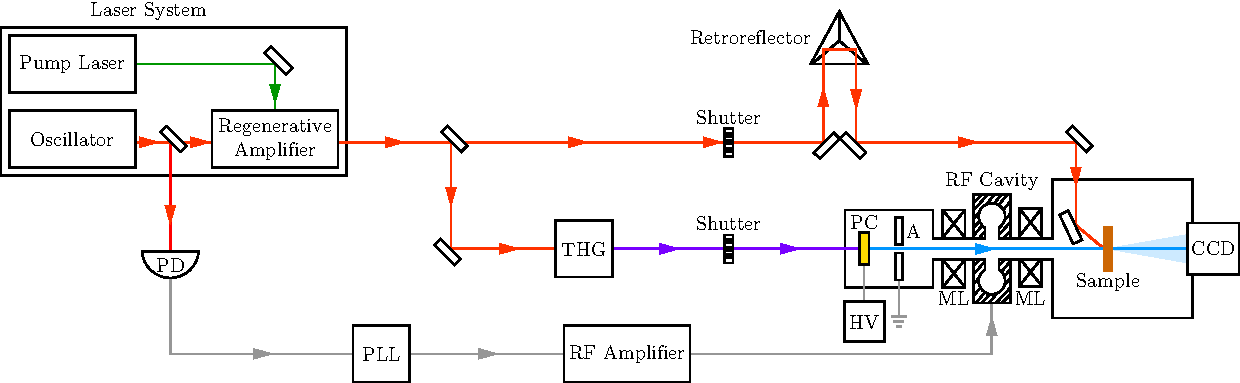
\includegraphics[width = \textwidth]{Figures/fig_ch2_setup-UED.pdf}
  \caption[Schematic of the experimental setup for UED.]{
    Schematic of the experimental setup for UED.
    For simplicity, it is not drawn to scale and minor components are not shown here.
    The black directional lines represent the paths of the electrical signals for
    synchronization, the blue one for the beam path of the electron pulses,
    the others are optical beam paths and their colour indicates the wavelength
    (green = 527 nm, red = 800 nm, and violet = 267 nm).
    Abbreviations: THG = third harmonic generation, PC = photocathode,
    A = anode, HV = high-voltage power supply, ML = magnetic lens, CCD = charge-coupled device,
    PD = photodiode, and PLL = phase-locked loop.
  }
  \label{fig: UED-setup}
\end{figure}

The UED experimental setup used in this thesis is depicted schematically
in Fig.~\ref{fig: UED-setup}. It can be divided up into two major segments:
a femtosecond laser system and an electron diffractometer.
The former is a Ti:Sapph laser system that operates on the same
principles as the commercial one used in the TA setup described in Sec.~\ref{sec: TA-setup}.
The latter is composed of an ultrabright DC-accelerated photoelectron source,
a RF pulse compression system, and a large vacuum sample chamber ($< 10^{-5}$~Pa air pressure)
with a sample holder and CCD~camera (Spectral Instrument~800) for imaging.

In a typical experiment, a Coherent Micra-5 laser acts as the oscillator,
producing a 800-nm, 75-MHz laser pulse train that is selectively amplified through CPA in
a Ti:Sapph REGEN pumped by a Q-switched Nd:YLF laser. The output pulses have a centre wavelength of 800~nm,
a pulse duration of 50~fs, a pulse energy of 0.5~mJ, and a repetition rate that can be
adjusted electronically from 10~Hz to 1~kHz. This light is split into the two beams, one for
pumping the sample and the other for generating the ultrafast electron probe pulses.
The pump beam is first time-delayed using a retroreflector mounted on a motorized translation stage,
focused, and then sent through a viewport of the sample chamber for photoexcitation of the sample.
Simultaneously, the probe beam is frequency-tripled to 267 nm through third harmonic generation%
\footnote{THG is a nonlinear optical process that triples the frequency of an input laser beam.
Here, it is achieved by first frequency-doubling the 800-nm input beam through SHG in a BBO~crystal,
temporally overlapping the 400-nm and remaining 800-nm light using a birefrigent calcite crystal,
and then combining them into 267-nm photons in another BBO~crystal
through sum frequency generation~(SFG).} (THG)
and focused onto a gold photocathode, from which electron pulses are emitted via the photoelectric effect%
\footnote{The photocathode in this setup is a 1-mm thick sapphire substrate with
20~nm of vapour-deposited gold,
which has a work function of ca.~3.8--4.3~eV~\cite{Tsang1991, Aidelsburger2010}.
considering the photon energy of the UV pulse, electrons would be emitted with excess kinetic energy
that translates to significant momentum spread.} with the same temporal profile.
The pulse energy of this UV laser beam is adjusted to be above
the saturation threshold (ca.~$110$ nJ, see Fig.~\ref{fig: electron-char1}a), ensuring that
laser power instability does not lead to fluctuation in the number of electrons per pulse.
%
\begin{figure}[t!]
 \centering
 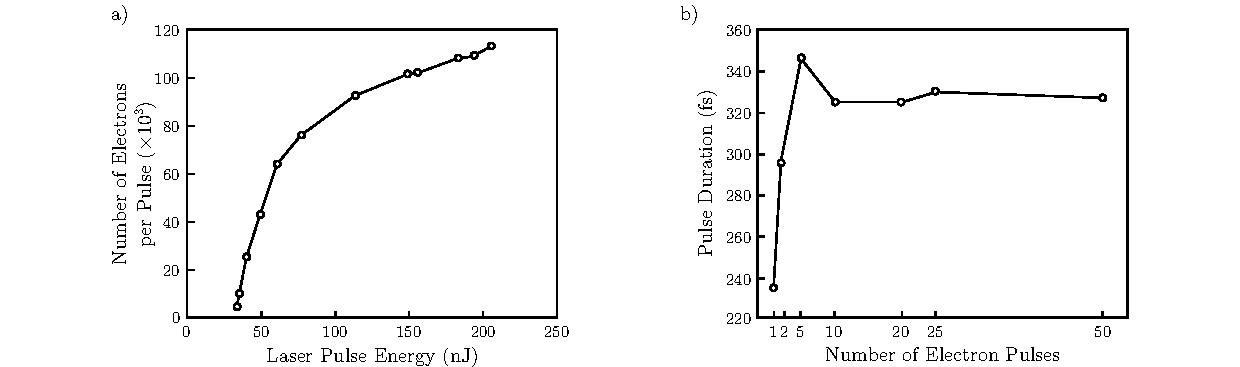
\includegraphics[width = \textwidth]{Figures/fig_ch2_electron-char1.pdf}
 \caption[Plots that illustrate some of the characteristics of the UED electron pulse.]{
   (a) The number of electrons emitted by the photocathode, as inferred by CCD counts,
   has a nonlinear dependence on the energy of the 267-nm laser pulse,
   hence a diminishing return above the saturation threshold.
   (b) Due to pulse-to-pulse variations in the arrival time of the electron pulses,
   the effective pulse duration increases and plateaus as a function of the number over
   which integration occurs.
   Adapted from Ref.~\cite{Yifeng-thesis} with permission of Dr.~Yifeng Jiang.
 }
 \label{fig: electron-char1}
\end{figure}
%
These electrons are accelerated over a distance of ca.~1~cm,
away from the photocathode (held at a potential of $-95$~kV by a high-voltage power supply)
and through a 200-$\unslant\mu$m pinhole%
\footnote{The pinhole blocks electrons that were generated with high transverse momentum;
its diameter can be increased to exchange better transverse beam coherence for higher beam brightness,
or vice versa.} in the anode (held at ground).
A magnetic lens collimates and directs them into a 3-GHz RF cavity.
Here, a time-varying electric field slows down the faster electrons at the front of the pulse and
speeds up the slower ones lagging behind,
thus longitudinally recompressing the pulses that have broadened substantially
due to Coulombic repulsion~\cite{Siwick2002}. As seen in Fig.~\ref{fig: RF-compression},
optimal compression is achieved by synchronizing the zero-crossing of the RF field
with the center of the electron pulses using a timing signal from the oscillator of the laser system;
phase stability is ensured through the use of phase-locked loop
synchronization electronics~\cite{Kiewiet2002}.
A second magnetic lens after the RF cavity focuses the electron beam onto the sample,
which is held in place by a custom holder, itself mounted on
a motorized three-axis linear translation and one-axis rotation stage system.
The transmitted electrons are finally detected by an highly sensitive CCD~camera,
wherein the image sensor is cooled to $-20$~$^{\circ}$C for a ultralow readout noise of
ca.~3~counts per pixel and directly coupled to a fiber plate coated in a layer of phosphor that
converts incident electrons into photons (ca.~100 counts per electron per pixel).
A thin layer of aluminium and carbon is also deposited on top of the phosphor
to filter out unwanted photons, such as those from the pump beam not absorbed by the sample.
The number of electron pulses over which the camera accumulates signal depends on
the time resolution needed for the experiment since the pulse-to-pulse timing jitter of
the electrons effectively broadens the pulse duration (see Fig.~\ref{fig: electron-char1}b).
%
\begin{figure}[t!]
  \centering
  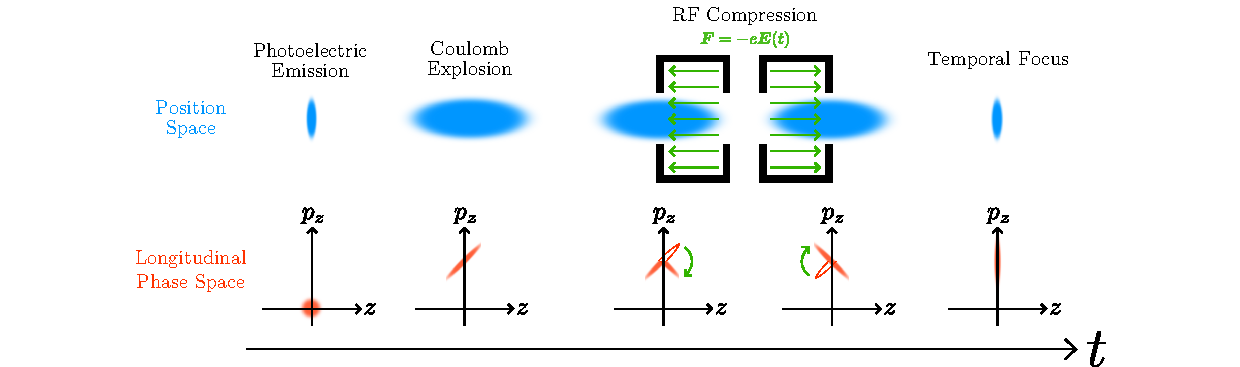
\includegraphics[width = \textwidth]{Figures/fig_ch2_RF-compression.pdf}
  \caption[The principle of RF electron pulse compression.]{
    The principle of RF electron pulse compression. An ultrafast electron pulse is emitted from
    the photocathode via the photoelectric effect and
    is accelerated by the DC electric field between the photocathode and the anode.
    It broadens longitudinally due to Coulombic repulsion and
    a linear velocity chirp develops in phase space as the faster electrons move ahead and
    the slower ones lag behind. During the propagation of the pulse through the RF cavity,
    a precisely synchronized time-varying electric field decelerates the leading electrons
    and accelerates the trailing ones, effectively rotating the electron distribution by
    $-90^{\circ}$ in phase space. Subsequent free-space propagation leads to
    optimal compression of the electron pulse at the sample position.
  }
  \label{fig: RF-compression}
\end{figure}

The electrons generated in this experimental setup have unique characteristics which
make them suitable for ultrafast electron diffraction. They are high energy%
\footnote{The electrons are high energy but not relativistic;
their Lorentz factor $\gamma = 1 + U/E_0$ is less than $2.0$ and
their relativistic beta $\beta = v/c = \sqrt{1 - 1/\gamma^2}$ is only 0.54.} ($95$~keV)
and thus have a de~Broglie wavelength (ca.~$0.038$~\AA) that is two orders shorter
than typical interatomic distances (e.g. $1.54$~\AA~for an average carbon--carbon bond~\cite{CRCBook}).
They are also packed into bunches in great numbers (ca.~$10^{5}$ e$^{-}$ per pulse),
resulting in a beam sufficiently bright to illuminate low-$Z$ materials and
produce high-quality diffraction patterns even at very low repetition rates.
%
A tight focus with a beamwidth of ca.~$200$~$\unslant\mu$m~FWHM at the sample position
is applied to maintain a high enough local transverse coherence width%
\footnote{The local transverse coherence width $L_T^{loc}$ is defined here as
$\hbar/\sigma_{p_x}^{\textrm{loc}}$, where $\sigma_{p_x}^{\textrm{loc}}$ is
the width of the electron momentum distribution in the transverse direction of the beam~\cite{AnnaSipe-thesis}.}
(ca.~$2$~nm, estimated using methods described in Ref.~\cite{Kirchner2013})
for diffraction off of most crystal lattices.
The `camera parameter'%
\footnote{The camera parameter is the conversion factor for the position of diffraction features,
between the camera frame (in pixels) and reciprocal space (in \AA$^{-1}$).
Although determined empirically here, it can be calculated as $4 \unslant[-.2]\pi l / (\lambda L)$,
where $l$ is the camera pixel size ($13.5$~$\unslant\mu$m/px),
$\lambda$ is the electron de~Broglie wavelength ($0.038$~\AA),
and $L$ is the sample-camera distance (ca.~$35$~cm).\label{fn: camera-parameter}}
is determined through calibration with the diffraction pattern of a known sample,
usually single-crystal silicon, and found to be ca.~$1.39 \times 10^{-2}$~\AA$^{-1}$/px.

The duration of the electron pulses is the most important quantity to optimize and
characterize in a UED setup since it strongly affects the ultimate time resolution of
the experiments and depends on a number of experimental parameters.
In the present setup, the pulse duration has been measured for each experiment
using a variety of different techniques. One approach involves measuring
the electron-laser pulse cross correlation~\cite{Siwick2005, Hebeisen2006, Gao2012}
by scattering the electron pulses off the ponderomotive potential generated
by two counter-propagating laser pulses,
a process known as the Kapitza-Dirac effect%
\footnote{Pyotr L. Kapitsa (1894--1984) and Paul A. M. Dirac (1902--1984)
developed the theory of electrons reflected by standing light waves in 1933~\cite{Kapitza1933}.
They were both awarded independently a Nobel Prize in Physics:
Kapitsa in 1978 for his work in low-temperature physics
(along with Arno A. Penzias and Robert W. Wilson
for their discovery of the cosmic microwave background radiation)~\cite{Nobel1971}
and Dirac in 1933 (jointly with Erwin Schr\"{o}dinger)
for a fully relativistic quantum theory~\cite{Nobel1901}.}~\cite{Freimund2001}.
When applied to the current UED setup, this technique yielded an estimate of the pulse duration
in the form of an IRF time of $(430 \pm 75)$~fs~FWHM~\cite{Gao2012}.

\begin{figure}[ht!]
  \centering
  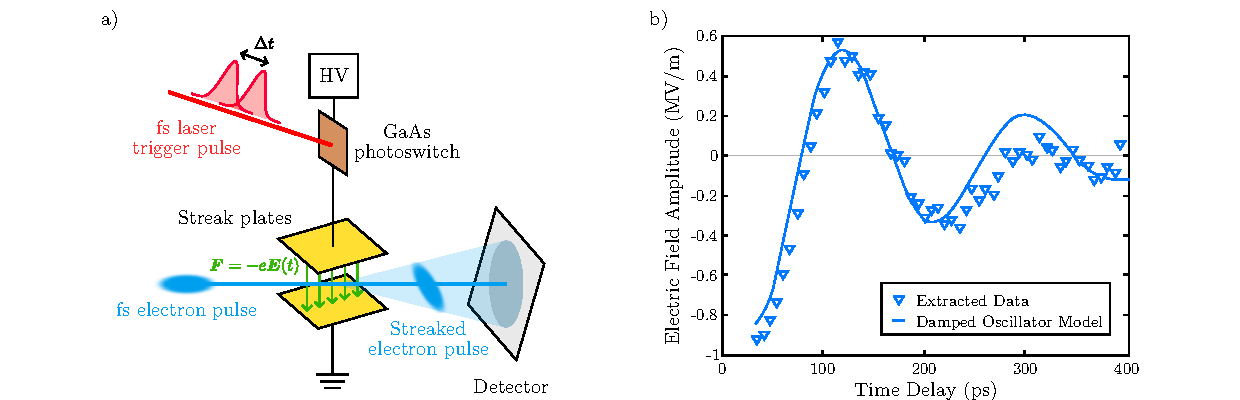
\includegraphics[width = \textwidth]{Figures/fig_ch2_streak-camera.pdf}
  \caption[The principle of electron pulse characterization by streak camera.]{
    The principle of electron pulse characterization by streak camera.
    (a) An ultrafast electron pulse propagating through the gap between the plates of the streak camera
    is deflected transversely by a time-varying electric field triggered by a 800-nm femtosecond laser pulse
    incident on a GaAs photoswitch. The temporal profile of the electron pulse is thus projected
    as the spatial profile of a traverse feature on the camera sensor.
    (b) The electric field between the streak plates oscillates and varies as a function of time delay
    between the trigger laser and the electrons.
    Adapted with permission from Ref.~\cite{Kassier2010}.
  }
  \label{fig: streak-camera}
\end{figure}

Although very precise, the ponderomotive scattering technique is not the one used to
characterize the pulses involved in the work of this thesis.
Here, a compact and convenient device known as a `streak camera',
designed and built by Dr.~G\"{u}nther H. Kassier~\cite{Kassier2010},
is employed to determine the timing of the electron pulses and the associated jitter.
As illustrated in Fig.~\ref{fig: streak-camera}a,
the streak camera can be simply described as a parallel plate capacitor connected
to a pulsed HV~source (${\sim}1500$ V) through a gallium arsenide~(GaAs) wafer
which acts as a photosensitive switch.
A femtosecond laser pulse that is synchronized to the electron pulse illuminates the photoswitch and
triggers an oscillating electric field between the streak plates (see Fig.~\ref{fig: streak-camera}b).
The passing electrons are deflected by this time-varying traverse field and their
longitudinal, temporal profile is projected as a traverse, spatial one.
Optimal streaking is achieved by setting the time delay of the trigger laser pulse such that
the electron pulse propagates through the streak field about its first zero crossing,
taking advantage of the maximum voltage ramp while ensuring zero overall beam deflection.
The pulse duration $\tau_e$ and arrival time $t_e$ of the electrons can be calculated using
the following relations~\cite{Wang2009}:
%
\begin{equation}
\begin{aligned}
    \tau_e & = \frac{\sqrt{ w_\textrm{st}^2 - w_\textrm{un}^2 }}{v_\textrm{st}} \\
    t_e & = \frac{y_\textrm{st} - y_\textrm{un}}{v_\textrm{st}}
\end{aligned}
\end{equation}
%
where $w_\textrm{s}$, $y_\textrm{s}$ are the beamwidth and centre position (in pixels)
of the electron spot on the camera sensor respectively,
given the streak status $s \in \{ \textrm{st: streaked}, \textrm{un: unstreaked} \}$;
$v_\textrm{st}$ is the streak velocity of the streak camera.
The latter is an important parameter to be characterized since it quantifies the time resolution
of the streak camera.
%
\begin{figure}[ht!]
  \centering
  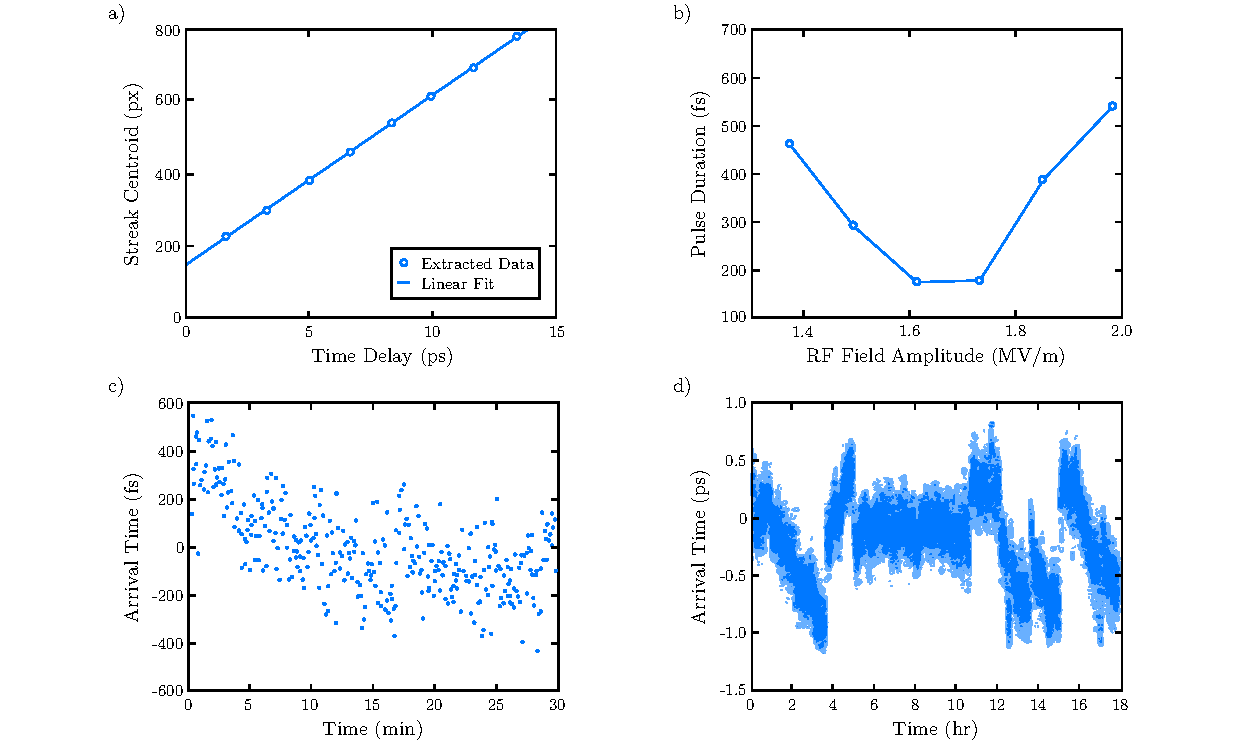
\includegraphics[width = \textwidth]{Figures/fig_ch2_electron-char2.pdf}
  \caption[The streak camera as a UED pulse timing tool.]{
    The streak camera as a UED pulse timing tool.
    (a) Streak velocity~$v_\textrm{st}$ is found as the fitted slope of the deflected position of the
    electrons with respect to the trigger laser time delay.
    (b) Optimal electron pulse compression is achieved by minimizing
    the pulse duration as a function of RF field amplitude.
    (c) Short-time jitter (ca.~$200$~fs~RMS) in the arrival time of the electron pulse.
    (d) Long-time drift in the arrival time monitored over several hours.
    Panel~a is adapted with permission from Ref.~\cite{Jiang2013} while
    Panels~b--f is from Ref.~\cite{Yifeng-thesis} with permission of Dr.~Yifeng Jiang.
  }
  \label{fig: electron-char2}
\end{figure}

In Fig.~\ref{fig: electron-char2}a,
$v_\textrm{st}$ is determined by varying the delay between the arrival time of the
trigger laser and the electron pulse and linearly fitting the centroid of the electron spot
as a function of time delay around the first zero crossing.
Here, it is found to be $(47.2 \pm 0.3)$ px/ps,%
\footnote{Considering the camera pixel size and sample-camera distance
(see Fn.~\ref{fn: camera-parameter}), this translates to a deflection velocity of ca.~$2.8$~mrad/ps.}
fast enough to allow for the single-pulse characterization of the timing of the electrons.
%
In Fig.~\ref{fig: electron-char2}b, the streak camera is used to measure
the single-shot pulse duration as a function of the RF field amplitude involved in electron pulse compression;
this is a key step in the preparation for UED data collection since this measurement is necessary
to determine the optimal field amplitude for maximum pulse compression ($< 200$ fs).
Furthermore, as seen in Fig.~\ref{fig: electron-char2}c and Fig.~\ref{fig: electron-char2}d,
short-time jitter and long-time drift of the arrival time of the electron pulse are monitored and
kept within 500~fs of the target time delay through adjustments of the phase of the RF field.

\begin{figure}[ht!]
  \centering
  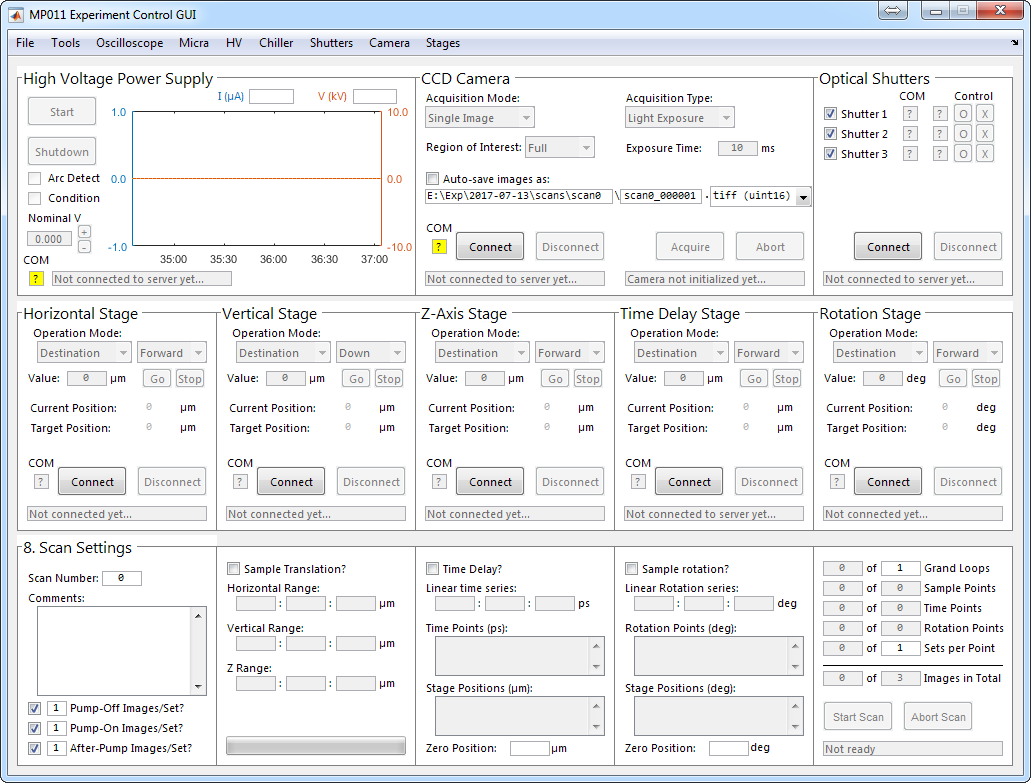
\includegraphics[width = \textwidth]{Figures/fig_ch2_MP011-app.png}
  \caption{
    Screenshot of the graphical user interface of the instrument control and data acquisition application
    that was built for the current UED experimental setup.
  }
  \label{fig: MP011-app}
\end{figure}
%
Beyond the ultrafast laser system and the electron diffractometer,
another key component of the UED setup is the computer program that
enables users to control the different instruments and acquire data.
Here, a full featured application software was developed from scratch
in the \textsc{MATLAB}~R2017b computing environment for this purpose.

Through the graphical user interface (shown in Fig.~\ref{fig: MP011-app}),
it is designed to send commands to and receive data from multiple instruments
hosted on computers connected in a distributed Ethernet network.
A purpose-built C++ server program running on the host computers translates
the TCP/IP packets sent by the control app to serial RS232 signals expected by
the instrument controller, and vice versa. A diagram of the architecture
is shown in Fig.~\ref{fig: MP011-net}.
This design is efficient
since interface- and device-specific functions are abstracted away into their respective applications,
modular since new instruments and users can be added and old ones removed
by simply creating new instances of the server and control apps,
and finally platform-independent since the chosen programming languages and communication protocols
are readily compatible to any modern operating system.
As such, this instrument control paradigm has superseded and replaced
an older, now obsolete scheme that was built using Visual Basic~6.0
as part of the doctoral work of Drs.~Maher Harb~\cite{Maher-thesis} and Meng Gao~\cite{Ray-thesis}.
%
\begin{figure}[ht!]
  \centering
  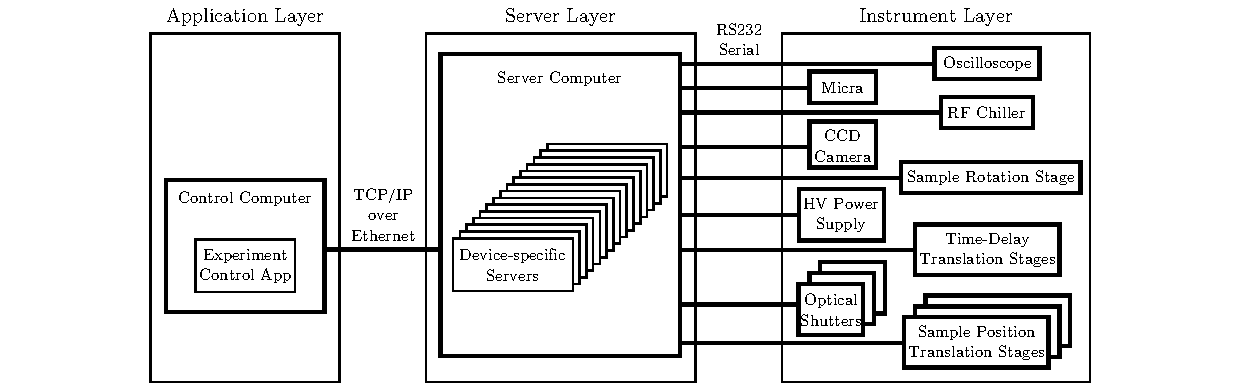
\includegraphics[width = \textwidth]{Figures/fig_ch2_MP011-net.pdf}
  \caption{
    Architecture of the software-hardware interface for instrument control and data acquisition.
  }
  \label{fig: MP011-net}
\end{figure}


%%%%%%%%%%%%%%%%%%%%%%%%%%%%%%%%%%%%%%%%%%%%%%%%%%%%%%%%%%%%%%%%%%%%%%%%%%%%%%%%%%%%

\subsection{Data Analysis --- Part 1}
\label{sec: UED-data-analysis-1}

Analysis of UED data is non-trivial.
%
Given that UED is a time-resolved pump-probe technique,
its data is inherently multidimensional, as in the case of of TA spectroscopy
(see Sec.~\ref{sec: TA-overview}).
A UED data `scan' is collected by scanning over a range of time delay
between the pump and probe pulses and,
for each time point, sets of electron diffraction patterns with alternating pump-shutter states
(`pump-on' and `pump-off') are recorded as high-resolution images.
These scans are then repeated as needed to improve the signal-to-noise ratio
and validate experimental conditions such as the pump laser fluence and sample temperature.
%
As a result, a typical experiment generates a large amount of data
in the form of hundreds of thousands of grayscale images,%
\footnote{
The images can be as large as the CCD~sensor of the camera ($2048 \times 2048$~pixels)
and they are stored as an uncompressed TIFF (`tagged image file format') 6.0 file;
the pixel values are unsigned 16-bit integers.}
%
each of which can be up to $8.4$~MB in size.
%
Hence, analysis of such a dataset --- maybe multi-terabytes in size ---
cannot follow the simplistic, ad hoc process of inspecting each image individually
for time-dependent features.
%
Instead, a `big data' approach%
\footnote{`Big data' herein refers to datasets that are too large to
fit entirely in the random-access memory of a typical personal computer (ca.~$8$~GB).}
to analytics is taken in the UED works presented in this thesis:
first preprocess and reduce, then model and interpret.

\begin{figure}[ht!]
  \centering
  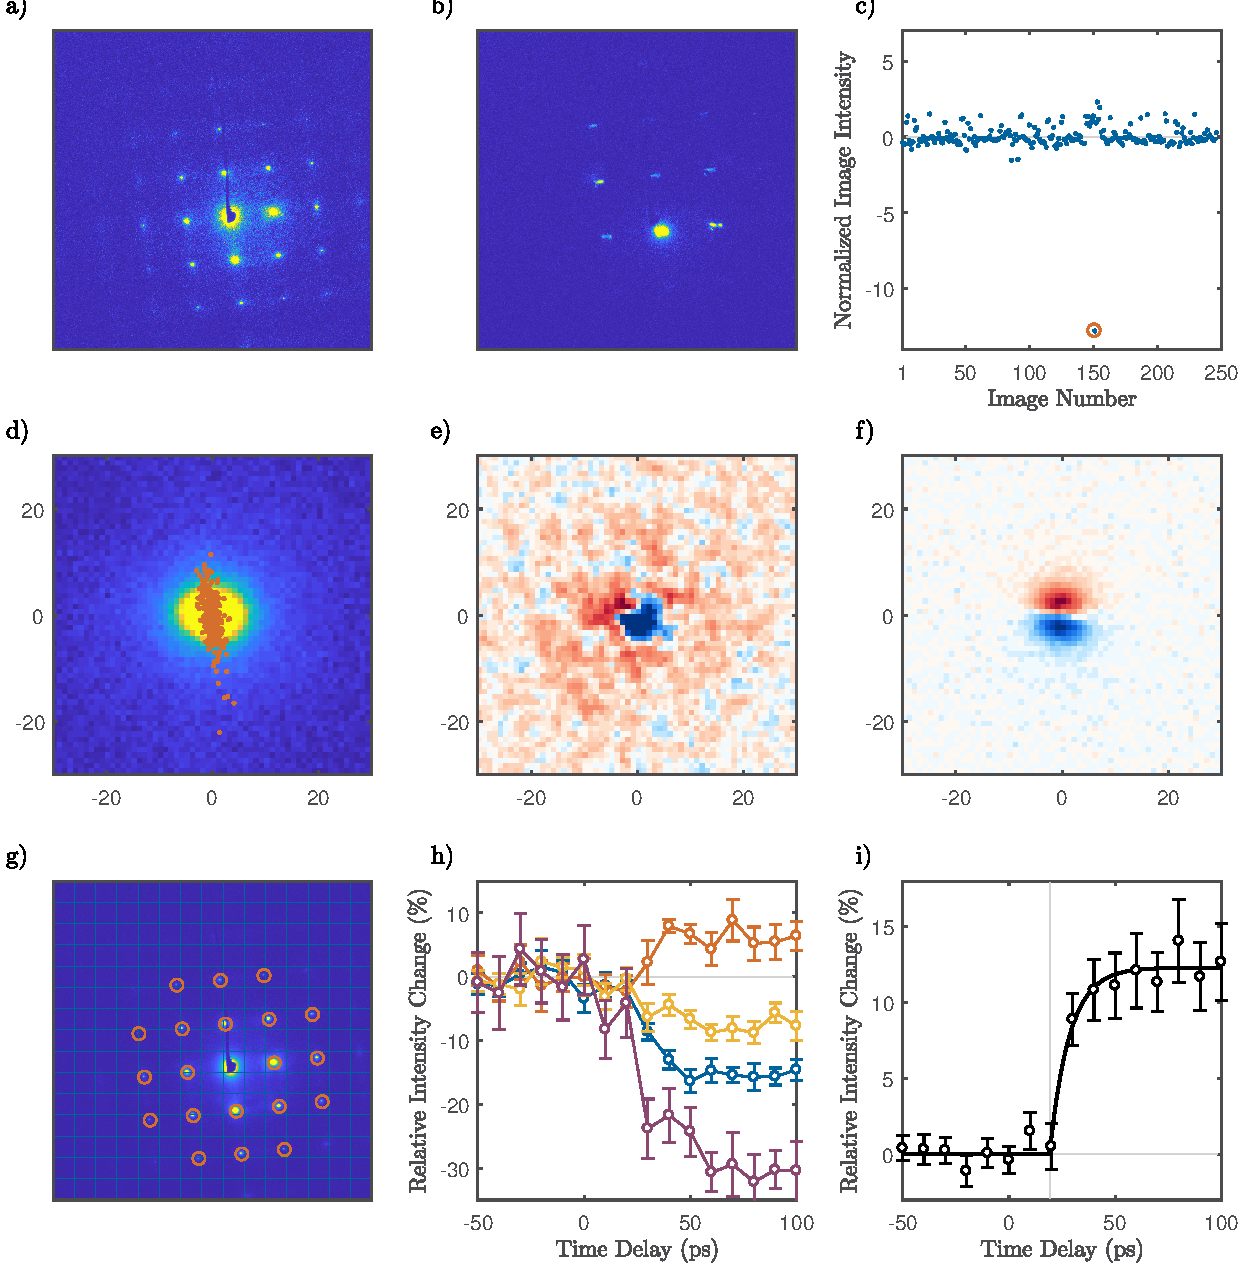
\includegraphics[width = \textwidth]{Figures/fig_UED_preprocess.pdf}
  \caption[Data preprocessing for a single UED scan.]{
  Data preprocessing for a single UED scan.
  Images need to be classified as either (a) nominal or (b) anomalous
  by calculating (c) the total image intensity and cleansing the outliers.
  (d) Beam-pointing instability (exaggerated by five times for clarity)
  is corrected by (g) finding all the visible diffraction spots,
  and using them as targets for motion tracking.
  For comparison, (e) the difference intensity distribution of (d) caused by photoexcitation
  is shown on the same colour scale with
  (f) that which results from a simulated subpixel vertical misalignment ($\delta q = 0.1$~px).
  (h) The image intensity at each visible diffraction spot is integrated and time traces $\Delta I(t)$
  are calculated; traces with $\text{SNR} > 1.5$ are accumulated and (i) fitted to
  a phenomenological signal function to determine $t_0$ of the scan.
  }
  \label{fig: UED-preprocess}
\end{figure}

% Find and reject bad images caused by arcs
Data preprocessing starts by cleansing the dataset of unreliable entries.
%
By inspection, there are obviously nominal and anomalous images,
e.g. Fig.~\ref{fig: UED-preprocess}a and b respectively.
%
The latter are those images acquired usually during anomalous exposure conditions,
caused by electrical discharge and arcing within the electron source assembly,
leading to sudden and large deviations in the electron beam brightness and energy.
These images need to be excluded to prevent the associated intensity variations
from obscuring the subtle changes induced by atomic motions.
%
Here, they are found and flagged by computing a normalized total intensity of every image
and discriminating any outliers from normal system noise.
Normalization of the intensity values is achieved by
subtracting a fitted smoothing spline as proxy for slow, unrelated fluctuations;
`outlier' refers to those data points
that are several standard deviations away from the median.
This process is showcased in Fig.~\ref{fig: UED-preprocess}c,
where the normalized intensity for the images of a sample UED scan is plotted
in multiples of standard deviation.

% Correct for drift caused by beam-pointing instability
Another source of noise that needs to be suppressed is the beam-pointing instability
of the laser beam that generates the UED electrons.
%
Since angular variation in the beam direction translates into
positional drift of the entire diffraction pattern,
pointing fluctuation that occurs between the acquisition of the pump-on and pump-off images
can conjure up changes in intensity that are unrelated to any photoinduced process.
%
Assuming a diffraction spot that is Gaussian in profile,
$I(\boldsymbol{q}) \propto \text{e}^{-\frac{1}{2}q^2 / \sigma^2}$,
and is displaced by some $\delta q \ll \sigma$,
the resulting relative change in intensity can be estimated by
%
\begin{equation}
  \begin{aligned}
      \max\limits_{\boldsymbol{q}}
        & \left\lvert \frac{I(\boldsymbol{q} - \delta \boldsymbol{q}) - I(\boldsymbol{q})}{I(\boldsymbol{q})} \right\rvert
        & \approx \frac{\delta q}{\sigma}
  \end{aligned}
\end{equation}
%
where the maxima are found at $q \pm \sigma$ along $\delta \boldsymbol{q}$.
%
For the diffraction spot displayed in Fig.~\ref{fig: UED-preprocess}d,
with~$\sigma = 4.4$~px, a subpixel displacement~($\delta q = 0.1$~px) introduces
a false signal~($\delta q/\sigma \approx 2.3$~\%)
comparable in magnitude to the real one~($|\Delta I/I_\text{off}| \approx 9.4$~\%),
hence the need for this data-preprocessing step.
%
Most of this problem is already mitigated through the use of an active pointing-stabilization mechanism%
\footnote{
A program authored by Dr.~Meng Gao actively monitors the pointing of the laser
by imaging a beam spot using a high-speed camera (PointGrey Firefly);
it then compensates for any significant deviation in spot position
by controlling a pair of in-beam mirrors mounted on piezoelectric actuators~\cite{Ray-thesis}.
}
that is setup along the optical beam path, immediately after the output of the laser system
(see Fig.~\ref{fig: UED-setup}).
%
However, this optomechanical solution is not perfect and
there are still significant shot-to-shot fluctuations in beam-pointing,
as seen in the positional jitter (ca.~$\pm 0.59$~px) shown in Fig.~\ref{fig: UED-preprocess}d.
%
To eliminate this leftover motion and further improve the SNR of the diffraction data,
some corrective techniques such as video stabilization are borrowed
from the field of computer vision.
%
First, the spots of the diffraction pattern are chosen as the targets for motion tracking.
These are automatically located within each image by first partitioning its area
into a regular array with a spacing less than the minimum inter-spot distance to ensure no concurrency
and then detecting features within each smaller area using image statistics.
A spot is deemed `present' if there is a pixel whose intensity value is the local maximum
and is greater than the local median by multiples (ca.~$30$) of the local standard deviation.
The centre position of the spot $\boldsymbol{q}_0$ is found by fitting
the intensity distribution of `spotty' areas to a general bivariate Gaussian function
%
\begin{equation}
  \begin{aligned}
      I(q_x, q_y)
        & = A \text{e}^{-\frac{1}{2}\left\lvert \mathbf{R} \left( \boldsymbol{q} - \boldsymbol{q}_0 \right)/\mathbf{\Sigma} \right\rvert^2} + B
  \end{aligned}
  \label{eq: gaussian-spot}
\end{equation}
%
where $\mathbf{R} = \mathbf{R}(\theta)$ is just the standard rotation matrix in two dimensions,
$\Sigma_{ij} = \sigma_i \delta_{ij}$, and
the set of fitting parameters is $\{ A, q_{0x}, \sigma_x, q_{0y}, \sigma_y, \theta, B \}$.
%
Fitted centre positions that are outside of the image area are discarded;
those that are closer together than half of the image partition width
are the result of overfitting near single spots and the redundant ones are also discarded.
%
Thus, all the searchable diffraction spots are found and their position is fixed over
every image of a scan.
%
The motion of each image is tracked and stabilized
by calculating the displacement of the centroid of its spot position from a reference point
and using this displacement vector to apply an image translation.
Translation by fractional pixel values is achieved by using a bilinear interpolation
of the image intensity values to calculate values at the translated pixel positions.
The result is a data scan wherein any photoinduced changes in diffraction features
can be directly and readily discerned from background noise (Fig.~\ref{fig: UED-preprocess}e).

Occasionally, a data scan would fail to exhibit any signal --- sigmoid-like changes in intensity
over time delay --- at any diffraction spot despite beam-pointing stabilization.
Such empty scans can be caused by a variety of experimental issues: a lack in spatial or temporal overlap
between the pump laser and the probe electron pulses, overly noisy pump and probe sources,
and sample degradation.
They need to be found and excluded from further analysis
to prevent SNR~loss when the entire dataset is ultimately averaged together.
%
This is achieved by first integrating the image intensity in each diffraction spot
and calculating their individual time trace~$\Delta I(t) = \frac{I_\text{on}(t) - I_\text{off}}{I_\text{off}}$
(Fig.~\ref{fig: UED-preprocess}h).
Traces whose values at $t \gg 0$ are statistically different from
those at $t \ll 0$ are averaged together to produce an overall time trace.
As in Fig.~\ref{fig: UED-preprocess}i,
signal is deemed to be present in a scan if its overall trace fits reasonably to
a Gaussian error function of the form $A \: \text{erf}\left(\frac{t-t_0}{\tau}\right) + B$,
where $t_0$ is the time-zero of the scan.

UED signals are not necessarily only found in the immediate area at and around the visible spots
of a diffraction pattern. Symmetry in a crystal structure causes `systematic absence'
or complete extinction of intensity of certain diffraction spots;
photoinduced structural dynamics can break such crystallographic symmetries
and scatter intensity into reciprocal lattice points
that were previously empty~\cite{Brefuel2009, Eichberger2010}.
%
A region-of-interest (ROI) search, more advanced than the earlier spot location analysis,
is thus performed to find and index the reciprocal lattice of the diffraction pattern.

To start, the beampointing-stabilized images are averaged to produce a reference image
to reduce shot noise. Further noise removal is done by applying
a two-dimensional adaptive Wiener filter%
\footnote{First proposed in 1949 by Norbert Wiener (1894--1964),
this image processing technique estimates the local mean and variance around each pixel
and then applies more or less smoothing in response~\cite{Lim1990}.} to the image.
%
Then, a mask is produced to specify areas of the UED image which are devoid of useful information
and need to be excluded from further analysis.
These include pixels that have been saturated, damaged, or shaded by a beam block.
Given that they are delimited by sharp intensity gradients, a Canny edge detector%
\footnote{This computational technique was developed by John F. Canny (1958--present) in 1986;
it detect edges by searching for connected pixels whose gradient magnitude is
between two given thresholds~\cite{Canny1986}.}
is used to trace their outline; a flood-fill pixel operation finds and fills the `holes'~\cite{Soille2004}.
In Fig.~\ref{fig: UED-rlattice}a, the outline of the beam block thus found is shown as a green line.

\begin{figure}[t!]
  \centering
  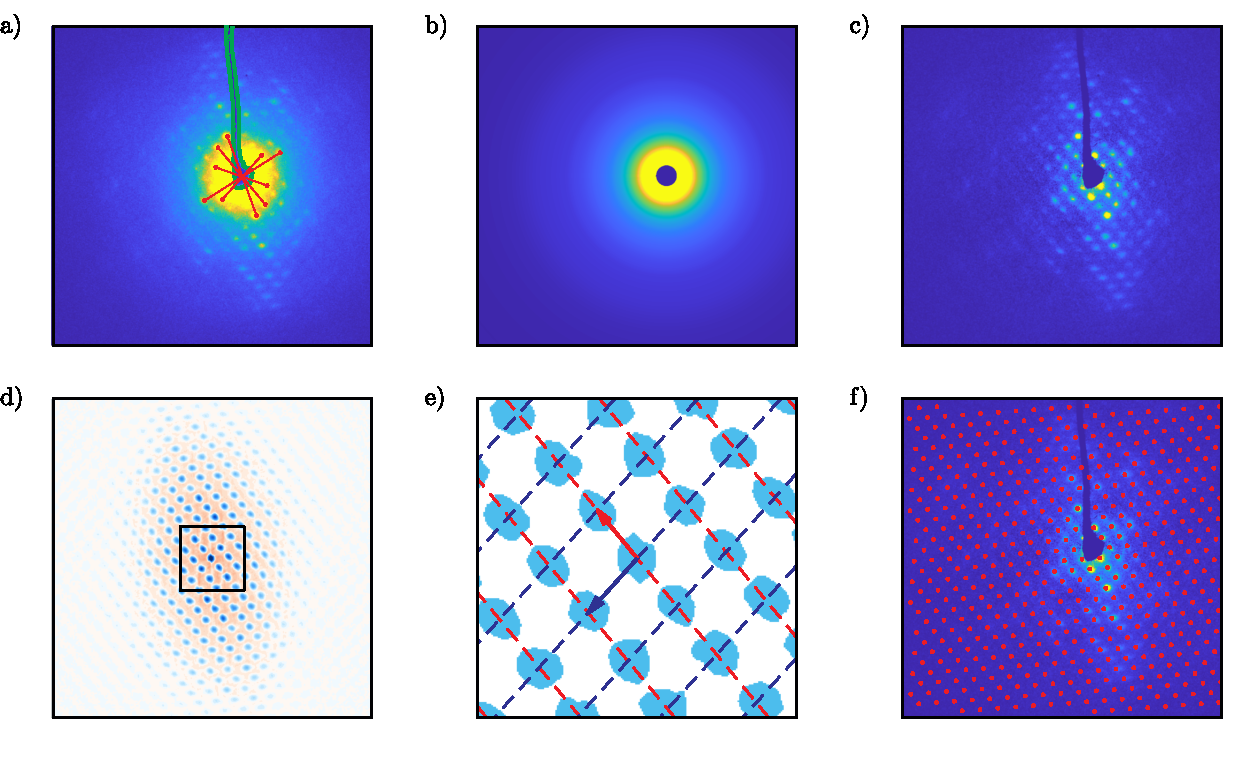
\includegraphics[width = \textwidth]{Figures/fig_UED_rlattice.pdf}
  \caption[Illustration of the steps of ROI search in a UED image.]{
  Illustration of the steps of ROI search in a UED image.
  %
  Step 1: construct a mask of any beam block by tracing its outline (green) with a Canny edge detector
  and determine the centre of the diffraction pattern from Friedel pairs (red).
  Step 2: estimate the intensity distribution of the transmitted beam (b)
  and subtract it from (a) to obtained a background-free image (c).
  Step 3: calculate the Laplacian of the autocorrelation of the image (d)
  and vectorize the centroid position of all the labeled connected regions (e).
  Step 4: position all the ROIs of the UED image (f)
  by generating a spanning grid from the lattice vectors found in (e).
  }
  \label{fig: UED-rlattice}
\end{figure}

To anchor the ROI search, the centre of the diffraction pattern needs to be found.
A rough estimate of its position is obtained by calculating the `centre of intensity' or
intensity-weighted arithmetic mean of the position of $>100$~random points
uniformly distributed over the masked image;
this is used to match diffraction spots into Friedel pairs%
\footnote{Named after Georges Friedel (1865--1933),
these pairs are the diffraction spots with Miller index $(h, k, l)$ and
$(\bar{h}, \bar{k}, \bar{l} )$~\cite{XRDBook}.}
amongst those found earlier.
By averaging the midpoint of the lines connecting these pairs of points,
a more accurate position of the centre is obtained.

With the centre of intensity found, subtraction of the background centered at $(000)$ can proceed
to enhance the intensity contrast between the diffraction spots and the transmitted beam.
%
Several techniques are known for performing this task
from literature (see Ref.~\cite{Downing2001} and the references therein);
however, they were found to be either ill-suited for automation or computationally labourious.
%
Here, given the isotropy of this intensity distribution, a coordinate transformation is applied
to the masked image that converts the Cartesian coordinates of its pixels to a set of polar ones
relative to the centre position. The pixels are then sorted in increasing order and
binned by their radial coordinate, rounded to the nearest integer.
The minimum intensity value within each bin is now taken to be the value of the background
at the prerequisite distance from the centre
as a mean to minimize the intensity contribution of the diffraction spots.
A background image (Fig.~\ref{fig: UED-rlattice}b) is reconstructed from this radial trace
by applying the reverse coordinate transformation and
using spline interpolation for non-integer radius values.
%
Hence, the background-free image (Fig.~\ref{fig: UED-rlattice}c) can be obtained
from the masked image (Fig.~\ref{fig: UED-rlattice}a).
%
Note that, in cases where the crystallinity of the sample and the quality of the electron beam
are poor, the diffraction spots can become so broad as to interfere
with the background subtraction algorithm, leaving faint ring-like artifacts.
%
Non-radial components of the background --- contributed by diffuse scattering due to crystal disorder ---
are left untreated here and may be dealt with using either a Fourier high-pass spatial filter
or an iterative model-based approach as described in Ref.~\cite{Grigorieff1995}.

Despite the preliminary noise removal and $(000)$-beam subtraction,
the ROI search is not performed directly on the background-free image.
As seen in Fig.~\ref{fig: plotDiffInt}, the diffraction pattern intensity
is effectively a periodic function $|S(\boldsymbol{q})|^2$ modulated by
a structural term $I_\text{st}(\boldsymbol{q})$.
The uneven modulation can result in the effective intensity extinction of low-order diffraction spots,
precluding a direct evaluation of the periodicity and indexing of the ROIs.
Here, this problem is solved by performing the ROI search instead on
a derived quantity $C(\boldsymbol{q}) = \nabla^2 \left( I(\boldsymbol{q}) \ast I(\boldsymbol{q}) \right)$,
where the convolution can be replaced by a sequence of fast Fourier transforms,
$I(\boldsymbol{q}) \ast I(\boldsymbol{q}) =
\mathcal{F}^{-1}\{ \mathcal{F}\{I(\boldsymbol{q})\}^2\}$.
%
Amongst the values of $C(\boldsymbol{q})$, the ROIs are now clearly visible
as a regular array of negative regions (Fig.~\ref{fig: UED-rlattice}e)
which are localized by masking all the positive regions, flattening the negative ones,
and applying `connected-component labeling'%
\footnote{This is performed using the \texttt{regionprops} function
in \textsc{MATLAB}~R2017b.} to the binary image.
%
Once labeled, the centroid of each array object is calculated and
the relative positions of the two non-collinear objects nearest to the image centre
can be used to define the two basis vectors necessary to index and specify
the position of every possible ROI within the diffraction pattern (Fig.~\ref{fig: UED-rlattice}f).

By integrating the intensity in the circular region centered at the positions found earlier,
the stack of pump-probe UED images of a data scan is reduced to a set of time traces.
Before the traces of multiple scans can be combined, their `clocks' need to be synchronized.
%
Significant drifts in the baseline arrival time of the probe pulse relative to that of the pump pulse
can occur as a result of scan-to-scan variation in environmental conditions,
which affects the timing electronics of the RF pulse compression system (Fig.~\ref{fig: UED-temp-vs-streak}).

\begin{figure}[t!]
  \centering
  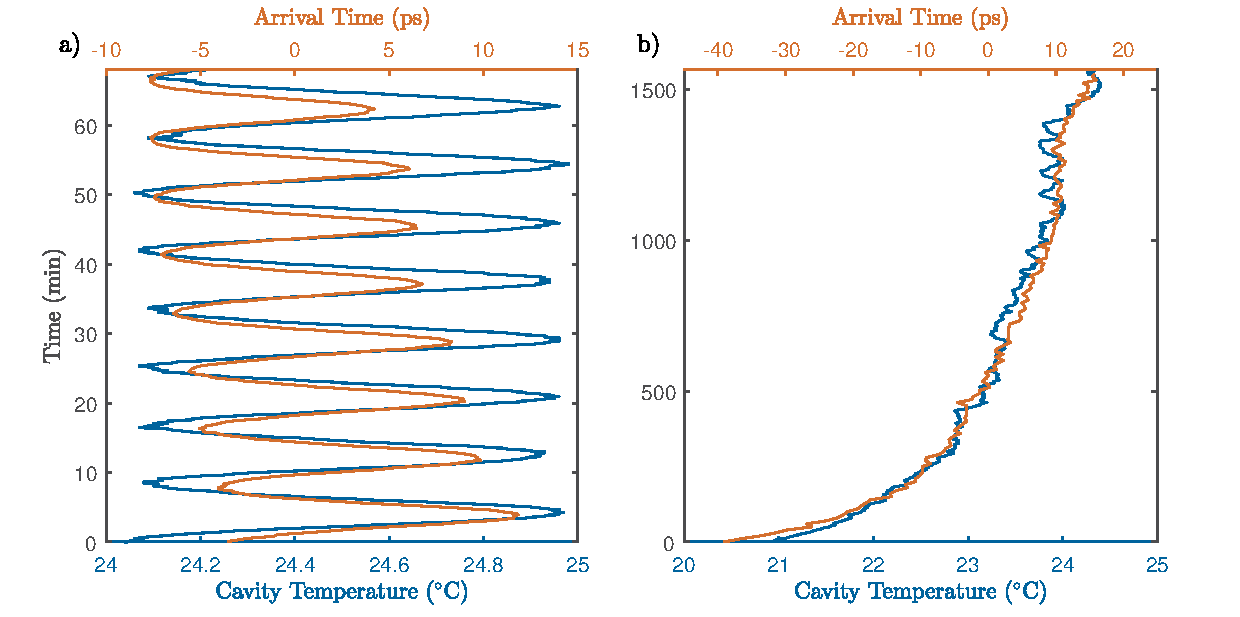
\includegraphics[width = \textwidth]{Figures/fig_UED_tempvsstreak.pdf}
  \caption[Correlation between the temperature of the RF cavity in the UED setup and
  the arrival time of the electron pulses under different conditions.]{
    Correlation between the temperature of the RF cavity in the UED setup and
    the arrival time of the electron pulses under different conditions.
    (a) The parameters of the proportional-integral-derivative~(PID) temperature controller
    for the RF cavity were intentionally detuned to generate oscillations.
    (b) Values were measured in the midst of the thermal equilibration of the UED setup.
  }
  \label{fig: UED-temp-vs-streak}
\end{figure}

To mitigate this issue, the time delay of each scan is shifted by the time-zero $t_0$
fitted during the data preprocessing step (Fig.~\ref{fig: UED-preprocess}i),
enabling the compilation of time traces measured
during different sessions of data collection (Fig.~\ref{fig: UED-rebin}a).
%
However, these traces cannot be directly averaged together
since the time points are now misaligned.
The solution is to treat the data like underexposed photographs and
apply an image processing technique known as `histogram equalization'
to enhance contrast by flattening the frequency distribution.
%
\begin{figure}[ht!]
  \centering
  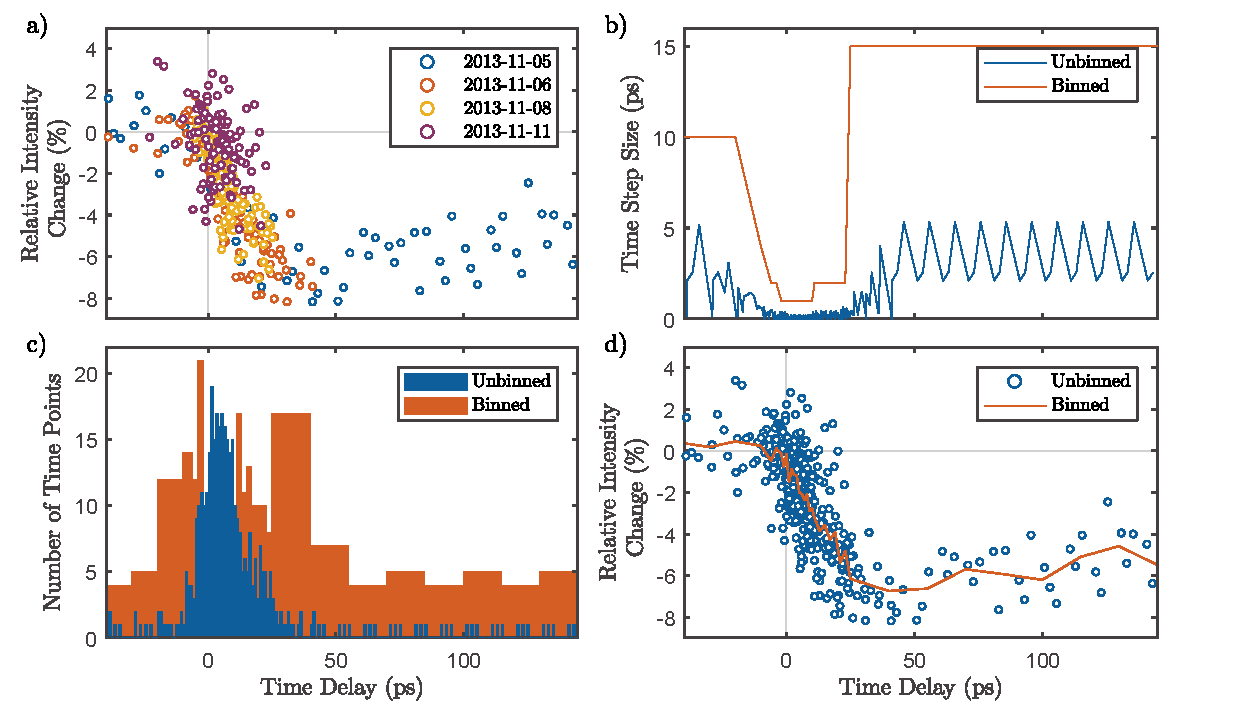
\includegraphics[width = \textwidth]{Figures/fig_UED_rebin.pdf}
  \caption[Combining UED data after time-zero correction with histogram equalization.]{
    Combining UED data after time-zero correction with histogram equalization.
    (a) Time traces from multi-day datasets cannot be directly averaged due to time point misalignment.
    A fix is to selectively choose (b) larger time steps, (c) broaden the sampling histogram.
    By calculating the mean of the data points within the new bins,
    (d) an average time trace can be obtained.
  }
  \label{fig: UED-rebin}
\end{figure}
%
As seen in the temporal sampling histogram (Fig.~\ref{fig: UED-rebin}c),
the distribution of time points is very narrow around the interval around $t = 0$,
i.e.~the temporal contrast of the compiled data is too low.
By choosing a new sampling scheme with selectively larger time steps,
equalization is achieved and a final noise-reducing average can then be taken
via a rebinning of the data point (Fig.~\ref{fig: UED-rebin}d).

%%%%%%%%%%%%%%%%%%%%%%%%%%%%%%%%%%%%%%%%%%%%%%%%%%%%%%%%%%%%%%%%%%%%%%%%%%%%%%%%%%%%

\subsection{Data Analysis --- Part 2}
\label{sec: UED-data-analysis-2}

At this point, further analysis of the UED data would traditionally involve
a mapping from reciprocal to real space by building a structure model.
This model would then be used to refine a set of reaction coordinates against
the diffraction intensities at each time point, thus producing a `molecular movie.'
%
Instead, a recognition could be that UED data
(changes in diffraction intensity $\delta I$ as a function of time $t$ and scattering vector $q$)
is structurally equivalent to TA data (changes in absorbance $\delta A$ as a function of time~$t$ and wavelength~$\lambda$)
and the structural dynamics as observed by UED can be elucidated within reciprocal space directly
through an analysis scheme comparable to that of TA.
%
This insight is grounded beyond the superficial similarity in functional dependence
but deeper in the dimensionality of the measurements.
%
In broadband TA spectroscopy, the number of sampled wavelengths is much greater than
the number of optically active species within the probe volume;
in UED of small molecules,
the number of observable diffraction spots, ca.~$400$, is similarly greater than
the number of degrees of freedom~(DOFs)%
\footnote{For the molecule (EDO-TTF)\textsubscript{2}PF\textsubscript{6},
there are $N = 35$ non-hydrogen atoms in the asymmetric unit, hence $3N-6 = 99$~DOFs.}
in the form of molecular translations, rotations, and vibrations.
In both cases, there is redundant complexity within the datasets that can be reduced
using singular value decomposition~(SVD).

\begin{figure}[t!]
  \centering
  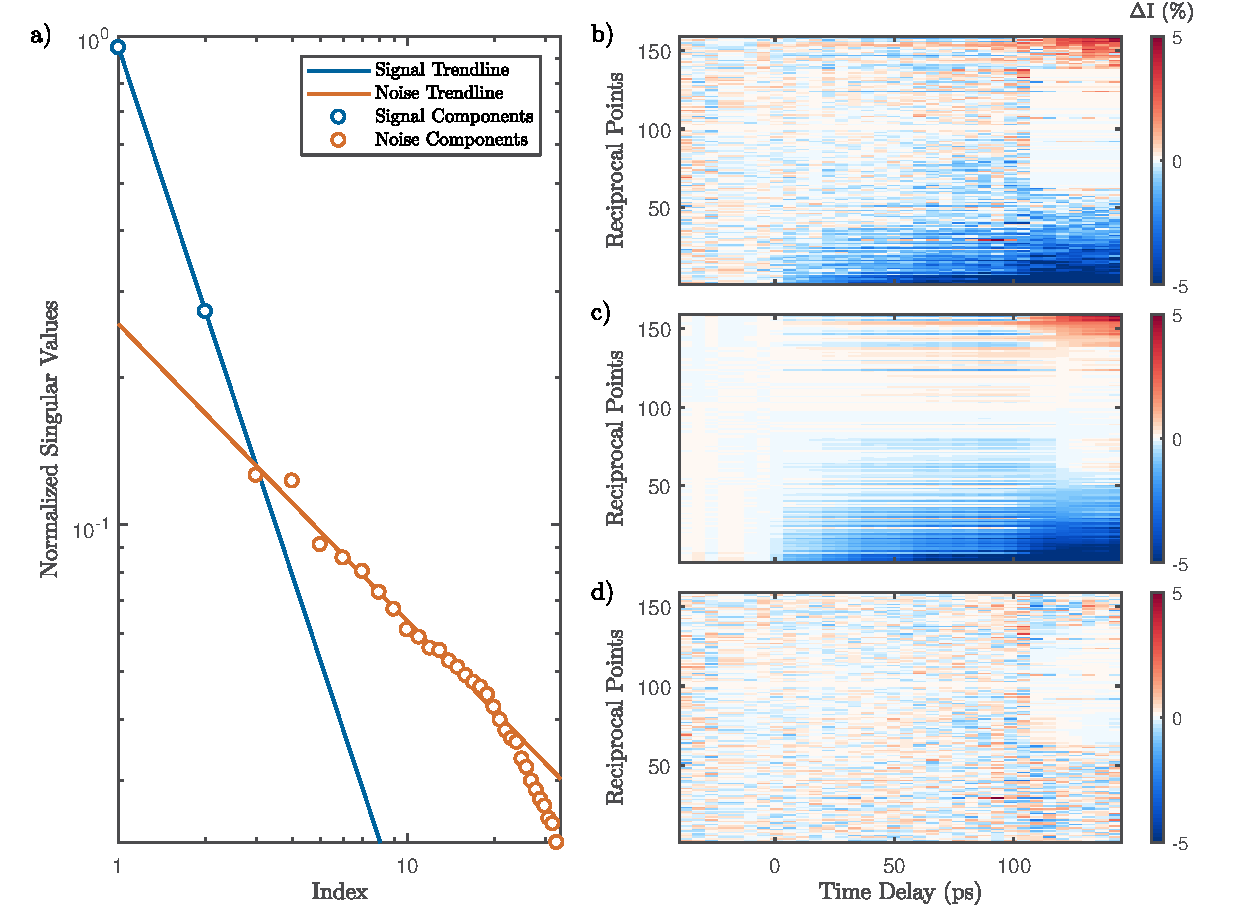
\includegraphics[width = \textwidth]{Figures/fig_UED_svd.pdf}
  \caption[Low-rank approximation of UED data matrix via singular value decomposition and truncation.]{
  Low-rank approximation of UED data matrix via singular value decomposition and truncation:
  (a) a log-log plot of the singular values $s_i$ shows that there are two types of singular components;
  (b) Time-dependent features are clearly present in the original data matrix but are partly obscured by noise;
  (c) summation of the terms before the dividing index $P'$, as per Eq.~\eqref{eq: UED-SVD}, returns a data matrix that is representative of
  the dynamics of interest;
  (d) summing those after yields data that is devoid of anything above SNR.
  }
  \label{fig: UED-svd}
\end{figure}

As in Sec.~\ref{sec: TA-data-analysis} and Fig.~\ref{fig: UED-svd}b, concatenate row-wise
the time trace of all diffraction spots, $\Delta I (t, \boldsymbol{q})$,
into a $M \times N$ data matrix $\mathbf{\Delta I}$,
$M$ and $N$ are the number of diffraction spots and time points respectively,
%
\begin{equation}
  \begin{aligned}
    %t & = \{ t_1, ..., t_N \} \\
    %\lambda & = \{ \lambda_1, ..., \lambda_M \} \\
    \Delta I(t, \boldsymbol{q}) \rightarrow \mathbf{\Delta I} =
    \begin{bmatrix}
        \Delta I(t_1, \boldsymbol{q}_1) & \cdots & \Delta I(t_N, \boldsymbol{q}_1) \\
        \vdots & \ddots & \vdots \\
        \Delta I(t_1, \boldsymbol{q}_M) & \cdots & \Delta I(t_N, \boldsymbol{q}_M)
    \end{bmatrix}
  \end{aligned}
\end{equation}
%
which can be factored via SVD into a linear combination of reciprocal-space and temporal features,
%
\begin{equation}
  \begin{aligned}
    \mathbf{\Delta I} & = \mathbf{U} \mathbf{S} \mathbf{V}^\mathsf{T} \\
      & = \sum_{i = 1}^P s_i \mathbf{u}_i \otimes \mathbf{v}_i^\mathsf{T}
    \label{eq: UED-SVD}
  \end{aligned}
\end{equation}
%
where $\mathbf{U} = \left[ \mathbf{u}_i \ldots \mathbf{u}_M \right]$
and $\mathbf{V} = \left[ \mathbf{v}_j \ldots \mathbf{v}_N \right]$ are orthogonal matrices
whose columns are the left and right singular vectors,
$\mathbf{u}_i = u_i(\boldsymbol{q})$ and $\mathbf{v}_j = v_i(t)$;
$\mathbf{S}$ is the $M \times N$ diagonal matrix of rank $P$ and whose diagonal elements $s_i$,
sorted in descending order, are the singular values of $\mathbf{\Delta I}$.
%
Given that the dynamics in UED data, as in TA~data, are effectively overdetermined,
a `low-rank approximation' of $\mathbf{\Delta I}$ is made
by truncating the sum of singular components $\mathbf{u}_i \otimes \mathbf{v}_i^\mathsf{T}$
at some $P' \ll P$.
As seen in a log-log plot of the singular values (Fig.~\ref{fig: UED-svd}a),
a flexure neatly segregates the major components from minor ones.
Given that the latter appear to be uncorrelated noises by inspection (Fig.~\ref{fig: UED-svd}d),
the penultimate index is chosen to be the value of $P'$,
yielding a data matrix that retains the dynamics of interest (Fig.~\ref{fig: UED-svd}c)
while losing the weakly contributing and undesirable features.

% Global analysis
To complete the global analysis of the UED data in reciprocal space,
a phenomenologically model function $f_i$ is chosen to fit $v_i(t)$,
the time-dependent part of each singular component (Fig.~\ref{fig: UED-svdfit}a).
Here, it is a linear combination of $Q$ exponential decay functions,
convolved with a Gaussian instrument response function
$\textrm{IRF}(t) = \text{e}^{- \frac{1}{2} t^2/\tau_\text{IRF}^2}$,
\begin{equation}
  \begin{aligned}
    f_i(t, \{ b_{i j}\}, \{k_j\})
        & = \sum_{j = 1}^Q b_{i j} \left( H(t) \text{e}^{-k_j t}\right) \ast \text{IRF}(t)
  \end{aligned}
  \label{eq: UED-GA}
\end{equation}
%
where $H(t)$ is the Heaviside function, $\tau_\text{IRF} \approx 180$~fs,
and $\tau_j = 1/k_j$ are the relevant time constants of the dynamics.%
\footnote{For reference,
$ \left( H(t - t_0) \text{e}^{-k t}\right) \ast \text{e}^{- \frac{1}{2} t^2/\tau^2} =
\frac{1}{2} \text{e}^{\frac{1}{2} k^2 \tau^2 - k (t - t_0)}
\left( 1 +
\text{erf}\left( \frac{t - t_0 - k \tau^2}{\sqrt{2} \tau} \right)
\right)$.
} In the case of the data shown in Fig.~\ref{fig: UED-svd},
only three exponential terms are necessary to produce good fits (Fig.~\ref{fig: UED-svdfit}a).
By re-summing the singular components using the fitted $v_i(t)$,
%
\begin{equation}
  \begin{aligned}
    G(t, \boldsymbol{q})
      & = \sum_{i = 1}^{P'} s_i u_i(\boldsymbol{q})
        \left( \sum_{j = 1}^Q b_{i j} \left( H(t) \text{e}^{-k_j t}\right) \ast \text{IRF}(t) \right)
  \end{aligned}
\end{equation}
%
a fit line $G(t, \boldsymbol{q})$ is produced for the time trace of
every sampled reciprocal point (Fig.~\ref{fig: UED-svdfit}b--d).

\begin{figure}[t!]
  \centering
  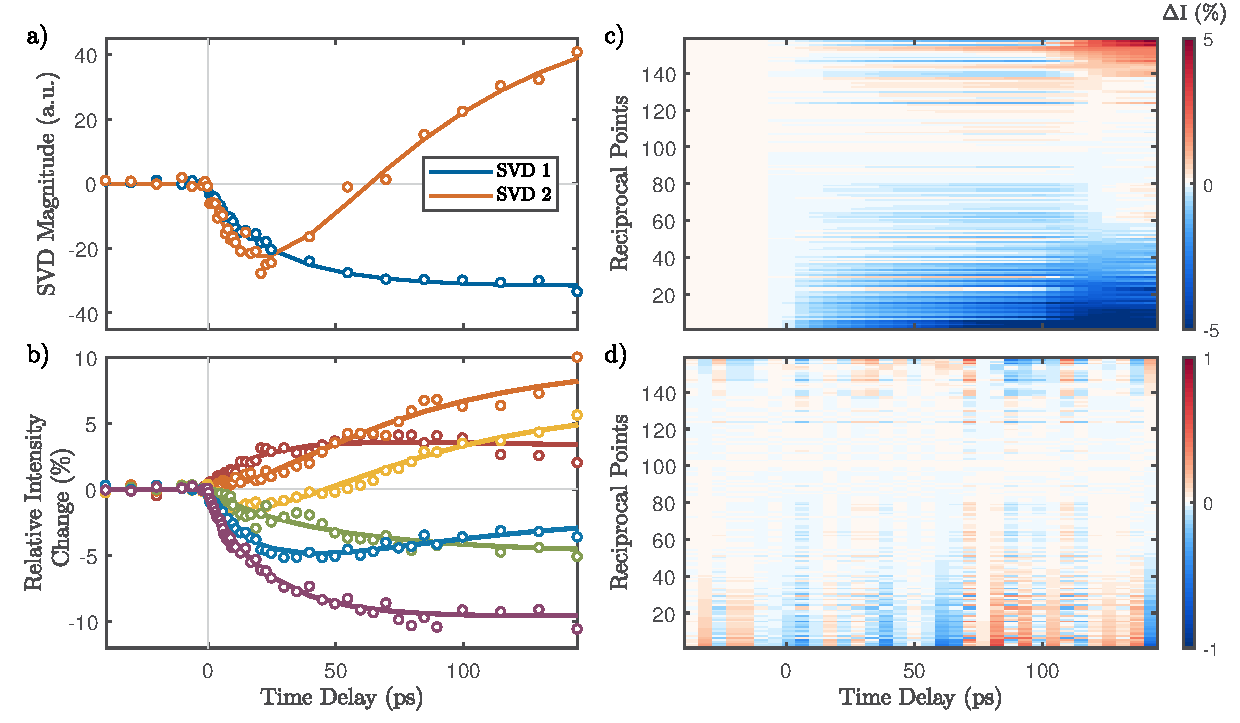
\includegraphics[width = \textwidth]{Figures/fig_UED_svdfit.pdf}
  \caption[Global analysis of UED data.]{
  Global analysis of UED data:
  (a) fitting of the principal right singular vectors $\mathbf{v}_i = v_i(t)$ is achieved
  using a few-parameter exponential model $f_i(t, \{ b_{i j}\}, \{k_j\})$ (see Eq.~\eqref{eq: UED-GA});
  the fitted parameters can then be used to reconstruct a global fit,
  i.e.~fit lines for all time traces;
  data for six select diffraction spots is shown in (b),
  and in (c), for all spots;
  the global residual is shown in (d).
  }
  \label{fig: UED-svdfit}
\end{figure}

% Talk about dimensionality reduction?

Another insightful and independent approach to analyzing UED data within reciprocal space directly
is to compute the Pearson correlation coefficient%
\footnote{Named after English mathematician Karl Pearson (1857--1936)~\cite{KarlPearson}.}
between the measured structure factors of the photoexcited molecule, $F_\text{exc}(t, \boldsymbol{q}_j)$,
with those of a reference, $F_\text{ref}(\boldsymbol{q}_j)$,
%
\begin{equation}
  \begin{aligned}
    P_\text{exc, ref}(t)
      & = \frac{\text{cov}(\zeta_\text{exc}(t, \boldsymbol{q}_j), \zeta_\text{ref}(\boldsymbol{q}_j))}{\sigma_\text{exc} \sigma_\text{ref}}
  \end{aligned}
  \label{eq: UED-Pearson}
\end{equation}
%
where
%
\begin{equation}
  \begin{aligned}
    \zeta_A(\boldsymbol{q}_j) & = \frac{F_A(\boldsymbol{q}_j)}{\bar{F}_A(\boldsymbol{q}_j)} - 1\\
    \text{cov}(\zeta_A, \zeta_B)
      & = \sum_{j = 1}^M \left( \zeta_A(\boldsymbol{q}_j) - \bar{\zeta}_A(\boldsymbol{q}_j) \right)
        \left( \zeta_B(\boldsymbol{q}_j) - \bar{\zeta}_B(\boldsymbol{q}_j) \right) \\
    \sigma_\text{A}
      & = \sqrt{\sum_{j = 1}^M \left(\zeta_A(\boldsymbol{q}_j) - \bar{\zeta}_A(\boldsymbol{q}_j) \right)^2} \\
  \end{aligned}
\end{equation}
%
and $\text{A}, \text{B}$ are the molecular states and
the overline indicates an arithmetic mean.
Given that the set of structure factors in a diffraction pattern is an expression of
the atomic coordinates of the target crystal structure,
the value of $P_\text{A, B}$ --- which varies from $-1$ to $1$ ---
quantifies the similarity between the molecular structure of two states.
In the case of a system with one or more known thermally accessible states $S_n$ beyond
the ground state $S_0$, a semblance of the space of all possible molecular configurations
can be constructed in the form of the Cartesian coordinates
$\left( P_\mathrm{X, S_0}, P_\mathrm{X, S_1}, \ldots, P_\mathrm{X, S_N} \right)$.
By following the time evolution of the point
$\boldsymbol{P}(t) = \left( P_\mathrm{exc, S_0}(t), P_\mathrm{exc, S_1}(t), \ldots,  P_\mathrm{exc, S_N}(t) \right)$,
the trajectory of the excited state through configuration space can be traced out.
This point is illustrated in Fig.~\ref{fig: UED-pearson} using the UED data of
(EDO-TTF)\textsubscript{2}SbF\textsubscript{6}.
%
\begin{figure}[t!]
  \centering
  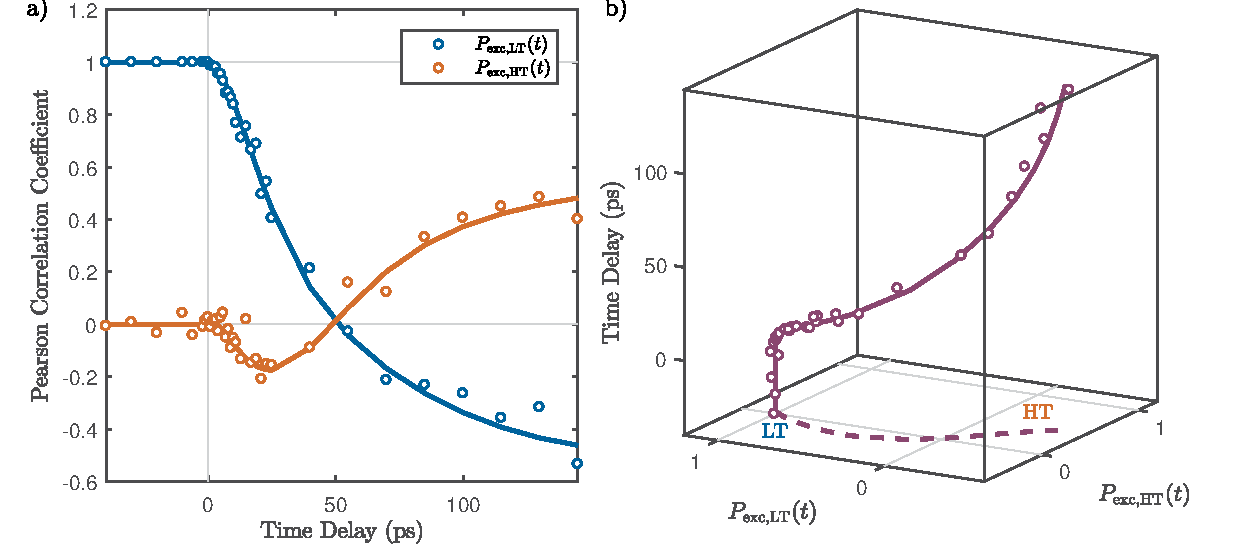
\includegraphics[width = \textwidth]{Figures/fig_UED_pearson.pdf}
  \caption[Pearson correlation analysis of UED data.]{
  Pearson correlation analysis of UED data:
  (a) computing the value of $P_\text{exc, ref}(t)$ for each of the two reference states (LT and HT)
  at each time point $t$ using Eq.~\eqref{eq: UED-Pearson};
  (b) plotting simultaneously the two sets of coefficients, rescaled such that $P_\mathrm{LT, HT}(t) = 0$,
  reveals the configurational pathway taken by the photoexcited molecule as it undergoes relaxation
  from the LT region (blue) to somewhere near the HT region (red).
  Note that these data points are derived from UED measurements made on
  crystals of (EDO-TTF)\textsubscript{2}SbF\textsubscript{6}.
  }
  \label{fig: UED-pearson}
\end{figure}
%
This molecule exists in its ground or `low temperature' (LT) state under normal conditions
undergoes a phase transition to a structurally distinct `high temperature' (HT) state
above 242~K (more details in Sec.~\ref{sec: UED-EDOSbF6}).
By correlating the measured diffraction intensities of the photoexcited state with those
of the LT and HT states, the molecule can be observed in Fig.~\ref{fig: UED-pearson}a
evolving away from its starting LT structure to a final product state structure
that is unexpectedly distinct from the HT structure.

Note that the Pearson correlation analysis requires as input the structure factors
of the photoexcited molecules, $F_\text{exc}(t, \boldsymbol{q}_j)$,
not those measured simply while the laser pump state is `on,' $F_\text{on}(t, \boldsymbol{q}_j)$.
%
To deconvolve these two quantities, it is necessary to make some assumptions about
the spatial distribution of the excited molecules in the crystal
on the microscopic scale~\cite{CoppensBook, Coppens1998, Coppens2005, Reeuwijk2000}.
In the case where strong photoexcitation or photoinduced cooperativity
generate many excited molecules that cluster together into sizable%
\footnote{On the order of the coherence length of the probe electrons} domains,
the structure factors are related by
%
\begin{equation}
  \begin{aligned}
    |F_\text{on}(t, \boldsymbol{q}_j)|^2
      & = \eta_\text{exc} |F_\text{exc}(t, \boldsymbol{q}_j)|^2
        + \left( 1 - \eta_\text{exc} \right) |F_\text{off}(\boldsymbol{q}_j)|^2
  \end{aligned}
\end{equation}
%
In the case of weak photoexcitation, the few excited molecules are randomly distributed
within an unperturbed lattice of ground state molecules,
an expression of the structure factors is instead given by
%
\begin{equation}
  \begin{aligned}
    F_\text{on}(t, \boldsymbol{q}_j)
      & = \eta_\text{exc} F_\text{exc}(t, \boldsymbol{q}_j)
        + \left( 1 - \eta_\text{exc} \right) F_\text{off}(\boldsymbol{q}_j)
  \end{aligned}
  \label{eq: coppens}
\end{equation}
%
where $\eta_\text{exc}$ is the excitation fraction.
Given that UED experiments are performed within a regime where
the fluence of the pump laser is relatively low and the sample response is linear,
the latter case is more likely. The absence of superlattice diffraction spots ---
associated with domain formation --- further suggests that the random-distribution model
is the appropriate choice for the works of this thesis.

Notice that $\eta_\text{exc}$ is still unknown and
one way to determine its value is using the crystallographic information and
the excitation conditions of the sample,
%
\begin{equation}
  \begin{aligned}
    \eta_\text{exc} = \frac{N_\text{exc}}{N_\text{tot}}
  \end{aligned}
  \label{eq: nexc-optical}
\end{equation}
%
The numerator $N_\text{exc}$ is the number of absorbed pump-laser photons that lead to photoexcitation,
%
\begin{equation}
  \begin{aligned}
    N_\text{exc}
      & = \left( \frac{E_\text{pump}}{h c / \lambda_\text{pump}} \right)
        \Phi \left( 1 - 10^{-A}\right) \text{erf}\!\left( \frac{w_\text{probe}}{\sqrt{2} w_\text{pump}}\right)
  \end{aligned}
\end{equation}
%
where $E_\text{pump}, \lambda_\text{pump}, w_\text{pump}$ are
the pulse energy, wavelength, and beamwidth of the pump laser,
$w_\text{probe}$ is the beamwidth of the probe electrons, and
$\Phi, A$ are the quantum yield and absorbance of the targeted transition;
the denominator $N_\text{tot}$ is the total number of absorbers
within the excitation volume of the pump laser,
%
\begin{equation}
  \begin{aligned}
    N_\text{tot}
      & = \frac{\unslant[-.2]\pi \left( \frac{1}{2} w_\text{probe} \right)^2 L}{V_\text{unit}} N_\text{abs}
  \end{aligned}
\end{equation}
%
where $L$ is the thickness of the sample, $V_\text{unit}$ is the volume of the crystal unit cell,
and $N_\text{abs}$ is the number of absorbers per unit cell.

A complementary way to determine $\eta_\text{exc}$ is possible
when the molecular system can arrive at the targeted product state via
a thermal phase transition as well as relaxation after photoexcitation.%
\footnote{This is true for all UED samples studied in this thesis,
with the exception of [Fe\textsuperscript{II}(bpy)\textsubscript{3}](PF\textsubscript{6})\textsubscript{2}
whose photoproduct state cannot be reached thermally.}
%
Since $\lim\limits_{t \rightarrow \infty} F_\text{exc}(t, \boldsymbol{q}_j) = F_\text{HT}(\boldsymbol{q}_j)$,
Eq.~\eqref{eq: coppens} becomes
%
\begin{equation}
  \begin{aligned}
    F_\text{on}(\infty, \boldsymbol{q}_j)
      & = \eta_\text{exc} F_\text{exc}(\infty, \boldsymbol{q}_j)
        + \left( 1 - \eta_\text{exc} \right) F_\text{off}(\boldsymbol{q}_j) \\
      & \approx \eta_\text{exc} F_\text{HT}(\boldsymbol{q}_j)
        + \left( 1 - \eta_\text{exc} \right) F_\text{LT}(\boldsymbol{q}_j)
  \end{aligned}
  \label{eq: coppens2}
\end{equation}
%
and then
%
\begin{equation}
  \begin{aligned}
    \eta_\text{exc} & = \frac{F_\text{on}(\infty, \boldsymbol{q}) - F_\text{LT}(\boldsymbol{q})}{F_\text{HT}(\boldsymbol{q}) - F_\text{LT}(\boldsymbol{q})}
  \end{aligned}
  \label{eq: nexc}
\end{equation}
%
Since the SNR of the denominator can be relatively small
for diffraction spots with less intensity or farther from the Bragg condition,
the output of this expression varies over different $\boldsymbol{q}_j$.
Restricting this calculation to the brightest diffraction spots on the Ewald sphere
yields a well-formed normal distribution and
a representative value for $\eta_\text{exc}$ is found as the median (Fig.~\ref{fig: UED-nexc}).

\begin{figure}[t!]
  \centering
  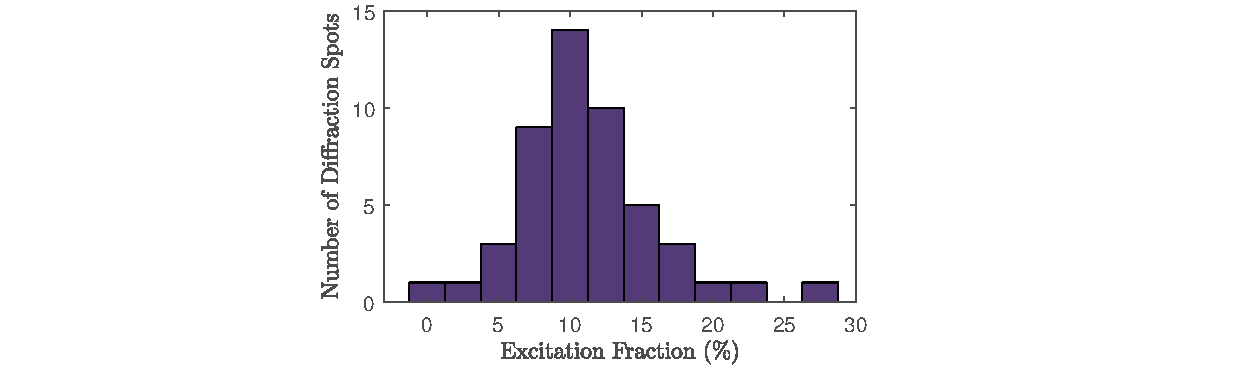
\includegraphics[width = \textwidth]{Figures/fig_UED_nexc.pdf}
  \caption{
  Histogram of the values of $\eta_\text{exc}$ determined by applying
  UED data to Eq.~\eqref{eq: nexc} when the photoproduct can be generated thermally.
  }
  \label{fig: UED-nexc}
\end{figure}

A third way to determine the excitation fraction can be used
if the molecular system exhibits significant changes in its lattice parameters
during the photoinduced and thermally-induced phase transitions.
In such a case, the spots of the diffraction pattern would shift in position
as the crystal lattice of the solid mixture distorts to accommodate
the two different sets of unit cells.
Assuming that the empirical rule known as Vegard's law%
\footnote{Norwegian physicist Lars Vegard (1880--1963) observed a linear relation between
the lattice parameters of ionic salt alloys and the concentration of each components
using XRD~\cite{Vegard1921, Denton1991}.}
%
holds in mixtures of photoexcited and ground state molecules,
a linear relation analogous to Eq.~\eqref{eq: coppens2}
can be stated as
%
\begin{equation}
  \begin{aligned}
    a_{j, \text{on}}(\infty)
      & = \eta_\text{exc} a_{j, \text{exc}}(\infty)
        + \left( 1 - \eta_\text{exc} \right) a_{j, \text{off}} \\
      & \approx \eta_\text{exc} a_{j, \text{HT}}
        + \left( 1 - \eta_\text{exc} \right) a_{j, \text{LT}}
  \end{aligned}
\end{equation}
%
and
%
\begin{equation}
  \begin{aligned}
    \eta_\text{exc}
      & = \frac{a_{j, \text{on}}(\infty) - a_{j, \text{LT}}}{a_{j, \text{HT}} - a_{j, \text{LT}}}
  \end{aligned}
  \label{eq: vegard}
\end{equation}
%
where $a_{j, \text{S}}$ is one of the three lattice parameters
in state $\text{S} = \{\text{on}, \text{off}, \text{HT}, \text{LT}\}$.

%%%%%%%%%%%%%%%%%%%%%%%%%%%%%%%%%%%%%%%%%%%%%%%%%%%%%%%%%%%%%%%%%%%%%%%%%%%%%%%%%%%%

\subsection{Data Analysis --- Part 3}
\label{sec: UED-data-analysis-3}

The data analysis of the original UED dataset has so far remained in the reciprocal space.
%
In Sec.~\ref{sec: UED-data-analysis-2}, data preprocessing has efficiently distilled
the multi-gigabyte stack of $\> 10^5$ UED images to
a single data matrix of relative intensity changes $\Delta I(\boldsymbol{t, q_i})$
integrated over the ROIs of the diffraction pattern.
%
In Sec.~\ref{sec: UED-data-analysis-3}, SVD-based global analysis reduced
the dimensionality of the data to a few key components that evolve over time;
calculation of the Pearson correlation coefficients projected
the evolving excited-state structure factors
$F_\text{exc}(\boldsymbol{t, q})$ as a trajectory
in the space of steady-state molecular configurations.
%
To finally make the titular `molecular movie' from the UED dataset,
a mapping from reciprocal to real space is necessary and
it is described in this section.

Recall from Eq.~\eqref{eq: Fsquared} that the crystal structure of a sample
could in principle be recovered by measuring its structure factors
$F(\boldsymbol{q}_j) = |F(\boldsymbol{q}_j)| \text{e}^{\text{i} \theta_j}$
and applying an inverse Fourier transform.
%
In practice, this is usually not possible
since the diffraction patterns of the sample is imaged by a CCD~camera
by simply counting the number of transmitted electrons and thus measuring only
the absolute value of the structure factors $|F(\boldsymbol{q}_j)|$.
%
Infamously known as the `phase problem' of crystallography,
the inaccessibility of the complex phases~$\theta_j$ means that
crystal structures are insufficiently constrained by their diffraction patterns
and cannot be uniquely determined so naively in general.
%
One solution is `molecular replacement':
replace the missing set of complex phases $\theta_j$ with values that
are derived from a structurally similar molecule (see Fig.~\ref{fig: phase-problem}
and Ref.~\cite{Taylor2003}).
%
In the works of this thesis, it is also the solution of choice since
the ground state structure of all the target molecules is already known
to a high degree of precision.
%
If there is a state $\text{S}_1$ proximate to the photoexcited state
that is either thermally accessible or metastable and long-lived,
an end structure would also be available in the literature;
a candidate structure with atomic positions $\bscriptr_{i, \text{exc}}$ for the transient state
that exists at each time point $t$ can then be modeled as a linear combination
of the two known structures,
%
\begin{equation}
  \begin{aligned}
    \bscriptr_{i, \text{exc}} & = \bscriptr_{i, \text{S}_0}
      + \xi_i \left( \bscriptr_{i, \text{S}_1} - \bscriptr_{i, \text{S}_0} \right)
  \end{aligned}
  \label{eq: linear-model}
\end{equation}
%
where $\xi_i$ is the scaling factor for the displacement of atom $i$ of $N_\text{at}$.

% Phase problem
\begin{figure}[t!]
  \centering
  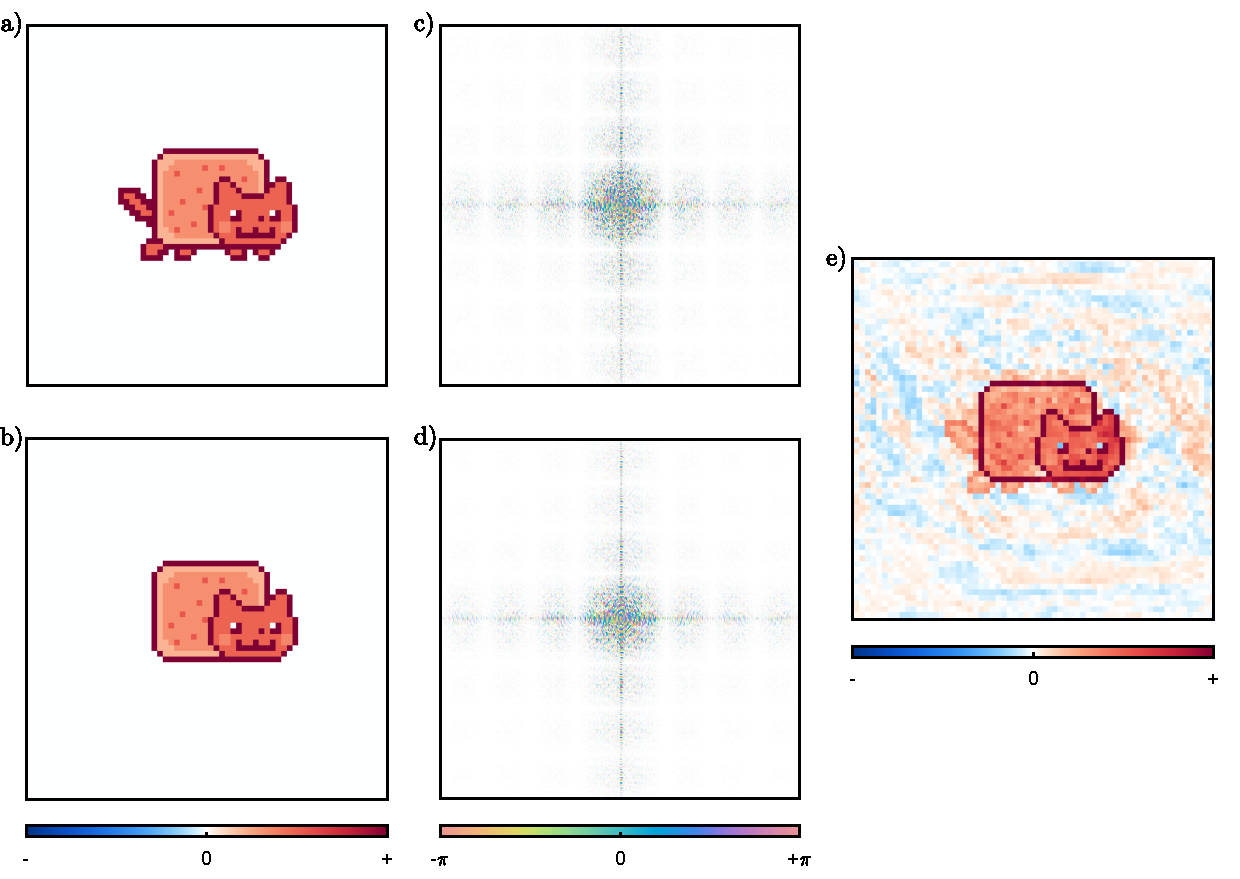
\includegraphics[width = \textwidth]{Figures/fig_ch2_nyancat.pdf}
  \caption[Phasing by molecular replacement.]{
    Phasing by molecular replacement.
    Electron diffraction maps the real-space electrostatic potential of the target
    into reciprocal space, here represented by (a)~a positive semi-definite image of a cat and
    (c)~its complex-valued Fourier transform.
    %
    Generally, information is partly lost when only the amplitude of the scattered wavefunction
    in the form of diffraction intensities is measured.
    %
    Given (b) a similar real-space distribution and (d) its known complex phase,
    the information loss can be reversed by phase substitution,
    resulting in (e) an hybrid that approximates the original.
  }
  \label{fig: phase-problem}
\end{figure}

To efficiently apply Eq.~\eqref{eq: Fsquared} and calculate the structure factors
of a given molecular model for a range of $\boldsymbol{q}$ values,
a popular analytical approximation of the electron elastic atomic scattering factors~$f(\boldsymbol{q})$
is used. From~\cite{Ren1996}, it is in the form of
%
\begin{equation}
  \begin{aligned}
    f_Z(\boldsymbol{q}) & = \sum_{n = 1}^6 a_n \text{e}^{- b_n (q/4 \unslant[-.2]\pi)^2}
  \end{aligned}
  \label{eq: fparameters}
\end{equation}
%
where $a_n, b_n$ are parameters fitted to the scattering data of each element with atomic number $Z$;
those used in the calculations of this thesis are plotted in Fig.~\ref{fig: UED-fparameters}
and tabulated in App.~\ref{ap: fparameters} for reference.

\begin{figure}[t!]
  \centering
  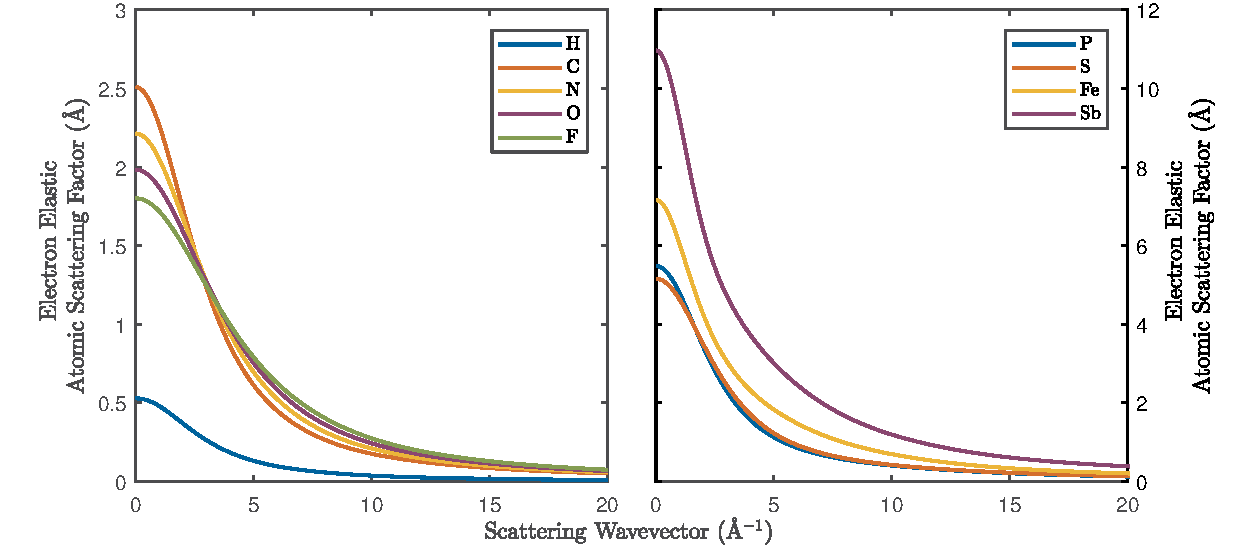
\includegraphics[width = \textwidth]{Figures/fig_UED_fparameters.pdf}
  \caption{
  Plot of the electron elastic atomic scattering factors $f(\boldsymbol{q})$ for select atoms,
  parameterized according to Eq.~\eqref{eq: fparameters}~\cite{Ren1996}.
  }
  \label{fig: UED-fparameters}
\end{figure}

% Diffraction pattern simulation
From Sec.~\ref{sec: UED-cryst}, the intensity distribution of
an electron diffraction pattern is shaped by more than just
the value of the structure factors of the sample.
%
As seen in Fig.~\ref{fig: ewald}b, experimental imperfections
affect the geometry of the scattering process and
consequently relax the Laue-Bragg condition for diffraction.
%
Thus, to generate an accurate set of diffraction intensities
for comparison with experimental results, a simulation scheme is setup in the way of
the Ewald construct, wherein the structure factor values are calculated at
the points $\boldsymbol{q}$ which are at the intersection of the Ewald sphere and
the reciprocal lattice $\boldsymbol{g}_{h_1 h_2 h_3} = \sum \limits_{i = 1}^3 h_i \boldsymbol{b}_i$.

The Ewald sphere constrains the calculation to the set of scattered wavevectors
permissible under elastic scattering,
%
\begin{equation}
  \begin{aligned}
    | \boldsymbol{q} - \boldsymbol{k}_\text{inc} | = k_\text{inc}
  \end{aligned}
\end{equation}
%
where $\boldsymbol{k}_\text{inc}$ is the wavevector of the incident probe electrons,
with amplitude $k_\text{inc} = \frac{2 \unslant[-.2]\pi}{\lambda}$ and
direction $\hat{\boldsymbol{k}}_\text{inc} \parallel \sum \limits_{i = 1}^3 u_i \boldsymbol{a}_i$.
%
Under this definition, the crystal orientation is held fixed while the incident direction
is referred by either $[ u_1, u_2, u_3 ]$ in the Miller notation%
\footnote{The letters $u, v, w$ are used most often to refer to crystal orientations;
however, numbered subscripts are used instead here for convenient indexing.}
or simply $\theta_\text{inc}, \phi_\text{inc}$ in spherical coordinates.

The points of the reciprocal lattice are modeled as Gaussian-shaped relrods.
Any $n$ relrods within the range of a diffraction spot cumulatively contribute
to the value of the structure factor at $\boldsymbol{q}$,
%
\begin{equation}
  \begin{aligned}
    f(\boldsymbol{q}) & = \text{e}^{-2W} \sum_{n} f(\boldsymbol{g}_n) \text{e}^{- \frac{1}{2} s_n^2 / \sigma^2}
  \end{aligned}
  \label{eq: relrods}
\end{equation}
%
where $\boldsymbol{g}_n$ is the position of the relrods near $\boldsymbol{q}$,
$s_n = |\boldsymbol{q} - \boldsymbol{g}_n|$ is the `excitation error' or
the deviation from the Laue-Bragg condition,
$W = \frac{1}{6} q^2 \left< \delta \scriptr^2 \right> $ is the Debye-Waller factor,
and $\sigma^2 = \sigma_\text{sh}^2 + (\sigma_\text{ph} q)^2$ is the width of the relrods;
$\sigma_\text{sh}$ is the contribution due to the shape factor $S(\boldsymbol{q})$ in
Eq.~\eqref{eq: diff-int} and $\sigma_\text{ph}$ is
a phenomenological parameter included to account for imperfections such as
crystal mosaicity and divergence of the probe beam.

To transform the $(q_x, q_y, q_z)$ coordinates in reciprocal space to the $(x, y, z)$ coordinates
of the UED images, a three-dimensional rotation is first made to align $\boldsymbol{k}_\text{inc}$
with $\hat{\boldsymbol{q}_z}$ using Rodrigues' rotation formula,%
\footnote{French mathematician Benjamin Olinde Rodrigues (1795--1851) discovered in 1840
this convenient formula to rotate a vector in three dimensional space
given an axis and an angle of rotation~\cite{Murray1994}.}
%
\begin{equation}
  \begin{aligned}
    \boldsymbol{q}
      & \rightarrow \boldsymbol{q} \cos \theta
        + (\hat{\boldsymbol{k}} \times \boldsymbol{q}) \sin \theta_\perp
        + \hat{\boldsymbol{k}} (\hat{\boldsymbol{k}} \cdot \boldsymbol{q}) (1 - \cos \theta)
  \end{aligned}
  \label{eq: rodrigues1}
\end{equation}
%
where $\hat{\boldsymbol{k}} = \frac{\hat{\boldsymbol{k}}_\text{inc} \times \hat{\boldsymbol{q}}_z}{ \sin \theta}$
and $\theta = \operatorname{arcos}(\hat{\boldsymbol{k}}_\text{inc} \cdot \hat{\boldsymbol{q}_z})$.
%
Alternatively,
%
%
\begin{equation}
  \begin{aligned}
    \boldsymbol{q} & \rightarrow \mathbf{R}(\theta) \boldsymbol{q}
  \end{aligned}
  \label{eq: rodrigues2}
\end{equation}
%
where
%
\begin{equation}
  \begin{aligned}
    \mathbf{R}(\theta) & = \mathbf{I} + \mathbf{K} \sin \theta  + \mathbf{K}^2 (1 - \cos \theta) \\
    \mathbf{K} & =
      \begin{bmatrix}
          0 & -k_z & k_y \\
          k_z & 0 & -k_x \\
          -k_y & k_x & 0
      \end{bmatrix}
  \end{aligned}
  \label{eq: rodrigues3}
\end{equation}
%
Finally, $\boldsymbol{q}$ is projected onto the camera frame and converted into units of image pixels
using the camera parameter (see Fn.~\ref{fn: camera-parameter}).

Altogether, the simulation of an electron diffraction pattern requires as input the following:
$N_\text{at} \times 3$ fractional atomic coordinates, the six lattice constants
($a_1, a_2, a_3$ and $\alpha_{23}, \alpha_{31}, \alpha_{12}$),
the camera parameter (${\sim}1.39 \times 10^{-2}$~\AA$^{-1}$/px),
the incident electron energy (95~keV) and direction $[u_1 u_2 u_3]$,
the Debye-Waller thermal variance $\left< \delta \scriptr^2 \right>$, and
the relrod widths $\sigma_\text{sh}, \sigma_\text{ph}$.
%
The value of the last six parameters are unique to each experiment and
they need to be determined with some precision.
%
This is achieved by first simulating the structure factors $F_\text{sim}(\boldsymbol{q})$
of the ground state using its known crystallographic information from XRD
for all possible orientations $\theta_\text{inc}, \phi_\text{inc}$
and maximizing the value of the Pearson correlation coefficient between the simulated
and experimental datasets $P_\text{sim, exp}$ (see Fig.~\ref{fig: UED-orientation}).
From this rough orientation, the other three parameters are refined using least-square fitting.

\begin{figure}[t!]
  \centering
  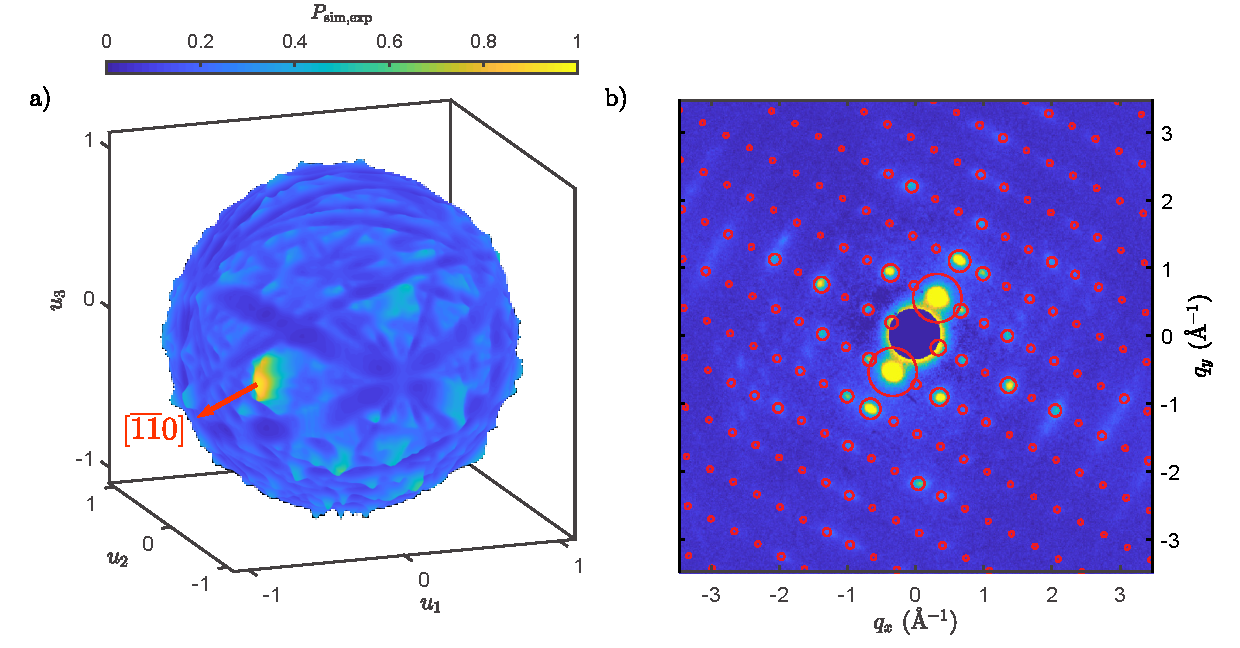
\includegraphics[width = \textwidth]{Figures/fig_UED_orientation.pdf}
  \caption[Determination of the incident direction of the probe electrons relative to the sample.]{
  Determination of the incident direction of the probe electrons relative to the sample:
  (a) for each possible direction, a diffraction pattern is simulated and compared with
  the experimental one by calculating their Pearson correlation coefficient $P_\text{sim, exp}$;
  (b) in the direction of peak correlation, there is optimal match between the simulated
  and experimental diffraction intensity. The size of the circles in Panel (b) is proportional to
  the value of $F_\text{sim}(\boldsymbol{q})$.
  }
  \label{fig: UED-orientation}
\end{figure}

% Molecular movie
Now that a scheme for accurately simulating UED data has been defined and optimized,
it can be applied to the structures generated by Eq.~\eqref{eq: linear-model}.
The resulting values of $F_\text{exc, sim}(\boldsymbol{\xi}, \boldsymbol{q}_j)$
are combined with the excitation fraction $\eta_\text{exc}$ in Eq.~\eqref{eq: coppens}
to produce simulated values that are representative of the `pump on' state,
%
\begin{equation}
  \begin{aligned}
    F_\text{on, sim}(\boldsymbol{\xi}, \boldsymbol{q}_j)
      & = \eta_\text{exc} F_\text{exc, sim}(\boldsymbol{\xi}, \boldsymbol{q}_j)
        + \left( 1 - \eta_\text{exc} \right) F_\text{off, sim}(\boldsymbol{q}_j)
  \end{aligned}
\end{equation}
%
which can then be compared with the time-dependent experimental structure factors values
$F_\text{on, exp}(t, \boldsymbol{q})$
--- extracted using the methods described in Sec.~\ref{sec: UED-data-analysis-2} ---
by calculating their Pearson correlation coefficient
%
\begin{equation}
  \begin{aligned}
    P_\text{sim, exp}(\boldsymbol{\xi}, t)
      & = \frac{\text{cov}(\zeta_\text{on, sim}(\boldsymbol{\xi}, \boldsymbol{q}_j), \zeta_\text{on, exp}(t, \boldsymbol{q}_j))}{\sigma_\text{on, sim} \sigma_\text{on, exp}}
  \end{aligned}
\end{equation}
%
and using it as a measure of the `goodness of fit' between the model structure
parameterized by $\boldsymbol{\xi}$ and the sought-after time-dependent structure of the photoexcited state.
%
Hence, to make the putative molecular movie, it is only a matter of maximizing
$P_\text{sim, exp}(\boldsymbol{\xi}, t)$ to find a $\boldsymbol{\xi}_\text{opt}(t)$
that reproduces the structural dynamics of the UED observations.
%
However, it is computationally too onerous to perform optimization on a function that
has so many independent variables, given that there are as many $\xi_i$ as atoms in the unit cell
of the sample.

A solution is to apply the principle of dimensionality reduction to aforementioned structure model.
From Sec.~\ref{sec: UED-data-analysis-2}, it can be argued that the plethora of redundant complexity in
reciprocal space suggests that molecular systems do not fully explore their configuration space
in all its $(3 N_\text{at} - 6)$-dimensional glory but instead live within a subspace spanned
by a few key reaction coordinates.
%
In this view, it is herein assumed that the $N_\text{at}$ atoms in the unit cell
can be partitioned into $N_G \ll N_\text{at}$ `dynamical groups'
within which member atoms move in lockstep, i.e. $\xi_i = \xi_j \enskip \forall \enskip i,j$ in
the group.
%
To determine which groupings amongst the infinitely many possible ones to test for optimization,
a first-principles approach based in `chemical intuition' can be employed as a preliminary to
future theoretical work involving quantum chemical calculations and molecular dynamics simulations.
%
It is recognized that molecules are generally composed of atoms or groups of atoms
which behave similarly whenever they occur in different compounds.
These assemblies are referred to as `functional groups' or `moieties' of the molecule
and those which preserve the symmetry of the unit cell constitute a reasonable guess of the dynamical groups
necessary to describe the observed structural dynamics.
%
This method is demonstrated in Fig.~\ref{fig: UED-molecularmovie} using the data
from the UED experiment on (EDO-TTF)\textsubscript{2}PF\textsubscript{6} (see Ch.~\ref{ch: UED-EDO}).

\begin{figure}[t!]
  \centering
  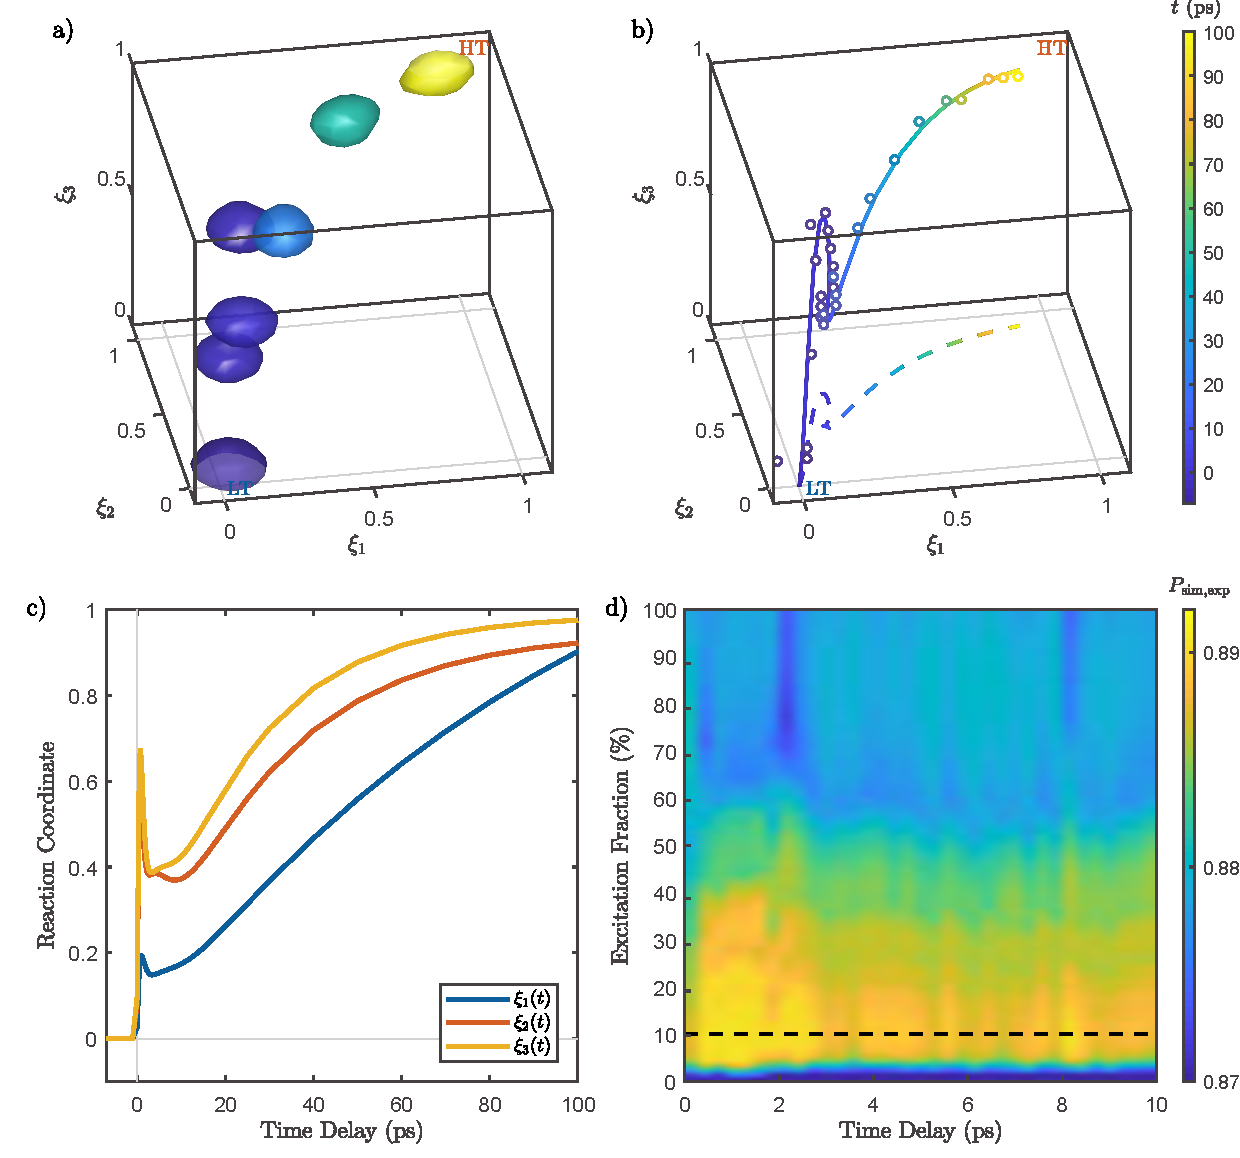
\includegraphics[width = \textwidth]{Figures/fig_UED_molecularmovie_.pdf}
  \caption[Making a molecular movie from UED data.]{
    Making a molecular movie from UED data:
    (a) isosurface plot of $P_\text{sim, exp}(\boldsymbol{\xi}, t)$ at different time delays
    in $\boldsymbol{\xi}$-space, with a cut-off at 95\% of the global maximum;
    (b) plot of $\boldsymbol{\xi}_\text{opt}(t)$ along with its fit line
    from a multi-exponential global fitting model;
    (c) plot of the fit lines of $\boldsymbol{\xi}_\text{opt}(t)$ as independent functions;
    (d) surface plot of $P_\text{sim, exp}(\boldsymbol{\xi}_\text{opt}, t)$ for a range of $\eta_\text{exc}$
    values, illustrating the temporal constancy of $\eta_\text{exc}$ and providing another way to confirm
    its value as calculated in Sec.~\ref{sec: UED-data-analysis-2}.
  }
  \label{fig: UED-molecularmovie}
\end{figure}

Three dynamical groups, parameterized by the reaction coordinates $\xi_1, \xi_2, \xi_3$, are constructed
by imposing inversion symmetry on the six moieties in the unit cell,
with the ground and end states specified by $\boldsymbol{\xi}  = (0, 0, 0)$ and $(1, 1, 1)$ respectively.
%
In Panels~(a)--(c), a well-behaved and strongly peaked $P_\text{sim, exp}(\boldsymbol{\xi}, t)$
can be seen in the space of $\boldsymbol{\xi} = (\xi_1, \xi_2, \xi_3)$,
suggesting that structural refinement at every time delay is readily achievable using this particular grouping;
in Panel~(d), optimization over $\eta_\text{exc}$ yields a sensible value that is consistent with
the calculations in Sec.~\ref{sec: UED-data-analysis-2} and
constant over the duration of the structural dynamics.
